\documentclass{standalone}
\begin{document}
\begin{table}[!htb]
	\centering
	\caption{Figure \ref{fig:graph_1001} Configuration File}
	\label{tab:graph_1001}
	\begin{tabular}{| c | c |}
		\hline
		Self Adaptive Offspring Count		& False		 \\
		\hline
		Tournament Size For Parent Selection		& 5		 \\
		\hline
		Penalty Coefficient		& 1		 \\
		\hline
		Runs		& 30		 \\
		\hline
		Parent Selection Algorithm		& k-Tournament Selection with replacement		 \\
		\hline
		Self Adaptive Mutation Rate		& False		 \\
		\hline
		Offspring Count		& 50		 \\
		\hline
		Termination Convergence Criterion		& 10000		 \\
		\hline
		Solution File Path		& None		 \\
		\hline
		Mutation Rate		& 0.1		 \\
		\hline
		Recombination Algorithm		& Partially Mapped Crossover		 \\
		\hline
		Random Seed		& 1001		 \\
		\hline
		Mutation Algorithm		& Move		 \\
		\hline
		Tournament Size For Survival Selection		& 5		 \\
		\hline
		Placement Algorithm		& Random		 \\
		\hline
		Population Size		& 100		 \\
		\hline
		Survival Strategy		& Plus		 \\
		\hline
		Search Algorithm		& EA		 \\
		\hline
		Log File Path		& None		 \\
		\hline
		Fitness Evaluations		& 10000		 \\
		\hline
		Survivor Algorithm		& Truncation		 \\
		\hline
		Self Adaptive Penalty Coefficient		& False		 \\
		\hline
	\end{tabular}
\end{table}
\begin{figure}[!htb]
	\caption{Input 1}
	\label{fig:graph_1001}
	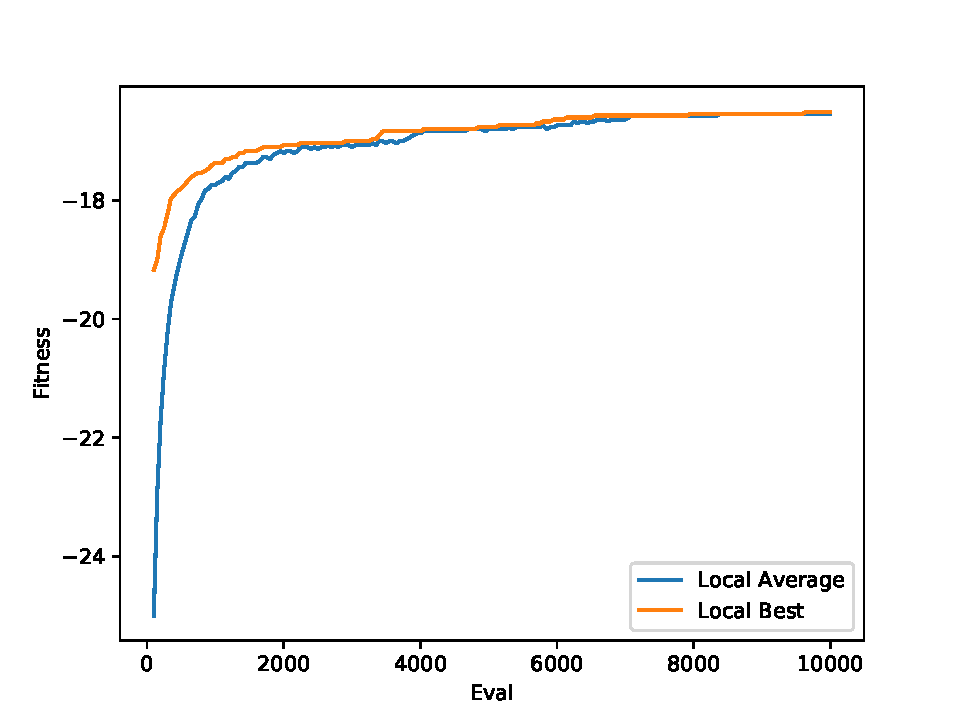
\includegraphics[width=\textwidth]{../graphs/graphs/1001.pdf}
\end{figure}


\begin{table}[!htb]
	\centering
	\caption{Figure \ref{fig:graph_1002} Configuration File}
	\label{tab:graph_1002}
	\begin{tabular}{| c | c |}
		\hline
		Self Adaptive Offspring Count		& True		 \\
		\hline
		Tournament Size For Parent Selection		& 5		 \\
		\hline
		Penalty Coefficient		& 1		 \\
		\hline
		Runs		& 30		 \\
		\hline
		Parent Selection Algorithm		& k-Tournament Selection with replacement		 \\
		\hline
		Self Adaptive Mutation Rate		& False		 \\
		\hline
		Offspring Count		& 50		 \\
		\hline
		Termination Convergence Criterion		& 10000		 \\
		\hline
		Solution File Path		& None		 \\
		\hline
		Mutation Rate		& 0.1		 \\
		\hline
		Recombination Algorithm		& Partially Mapped Crossover		 \\
		\hline
		Random Seed		& 1002		 \\
		\hline
		Mutation Algorithm		& Move		 \\
		\hline
		Tournament Size For Survival Selection		& 5		 \\
		\hline
		Placement Algorithm		& Random		 \\
		\hline
		Population Size		& 100		 \\
		\hline
		Survival Strategy		& Plus		 \\
		\hline
		Search Algorithm		& EA		 \\
		\hline
		Log File Path		& None		 \\
		\hline
		Fitness Evaluations		& 10000		 \\
		\hline
		Survivor Algorithm		& Truncation		 \\
		\hline
		Self Adaptive Penalty Coefficient		& False		 \\
		\hline
	\end{tabular}
\end{table}
\begin{figure}[!htb]
	\caption{Input 1}
	\label{fig:graph_1002}
	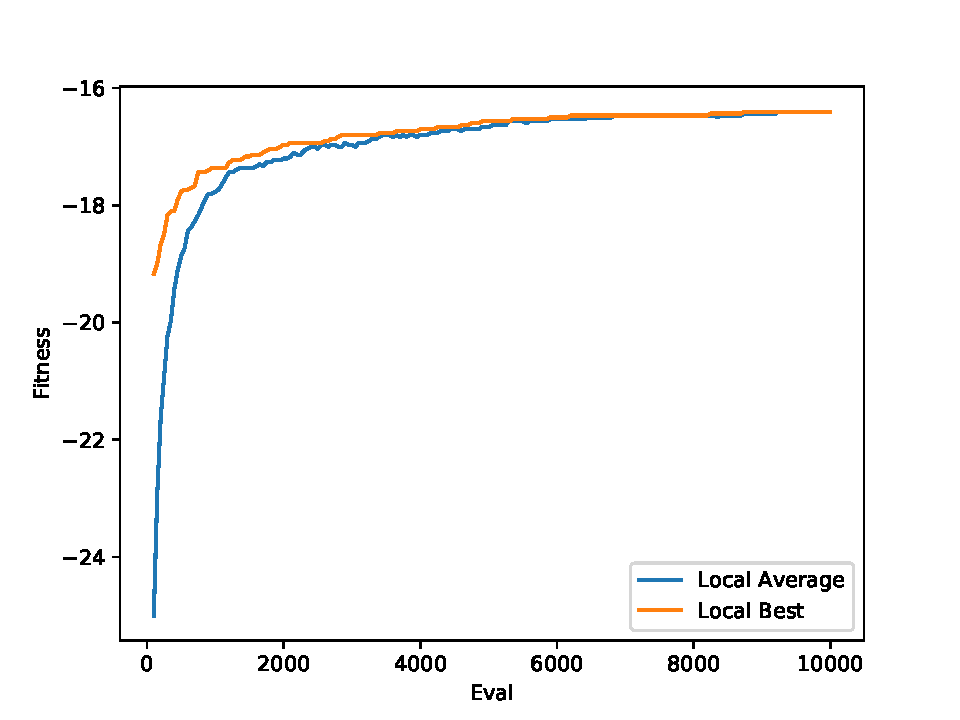
\includegraphics[width=\textwidth]{../graphs/graphs/1002.pdf}
\end{figure}


\begin{table}[!htb]
	\centering
	\caption{Figure \ref{fig:graph_1003} Configuration File}
	\label{tab:graph_1003}
	\begin{tabular}{| c | c |}
		\hline
		Self Adaptive Offspring Count		& False		 \\
		\hline
		Tournament Size For Parent Selection		& 5		 \\
		\hline
		Penalty Coefficient		& 1		 \\
		\hline
		Runs		& 30		 \\
		\hline
		Parent Selection Algorithm		& k-Tournament Selection with replacement		 \\
		\hline
		Self Adaptive Mutation Rate		& False		 \\
		\hline
		Offspring Count		& 50		 \\
		\hline
		Termination Convergence Criterion		& 10000		 \\
		\hline
		Solution File Path		& None		 \\
		\hline
		Mutation Rate		& 0.1		 \\
		\hline
		Recombination Algorithm		& Partially Mapped Crossover		 \\
		\hline
		Random Seed		& 1003		 \\
		\hline
		Mutation Algorithm		& Move		 \\
		\hline
		Tournament Size For Survival Selection		& 5		 \\
		\hline
		Placement Algorithm		& Random		 \\
		\hline
		Population Size		& 100		 \\
		\hline
		Survival Strategy		& Plus		 \\
		\hline
		Search Algorithm		& EA		 \\
		\hline
		Log File Path		& None		 \\
		\hline
		Fitness Evaluations		& 10000		 \\
		\hline
		Survivor Algorithm		& Truncation		 \\
		\hline
		Self Adaptive Penalty Coefficient		& True		 \\
		\hline
	\end{tabular}
\end{table}
\begin{figure}[!htb]
	\caption{Input 1}
	\label{fig:graph_1003}
	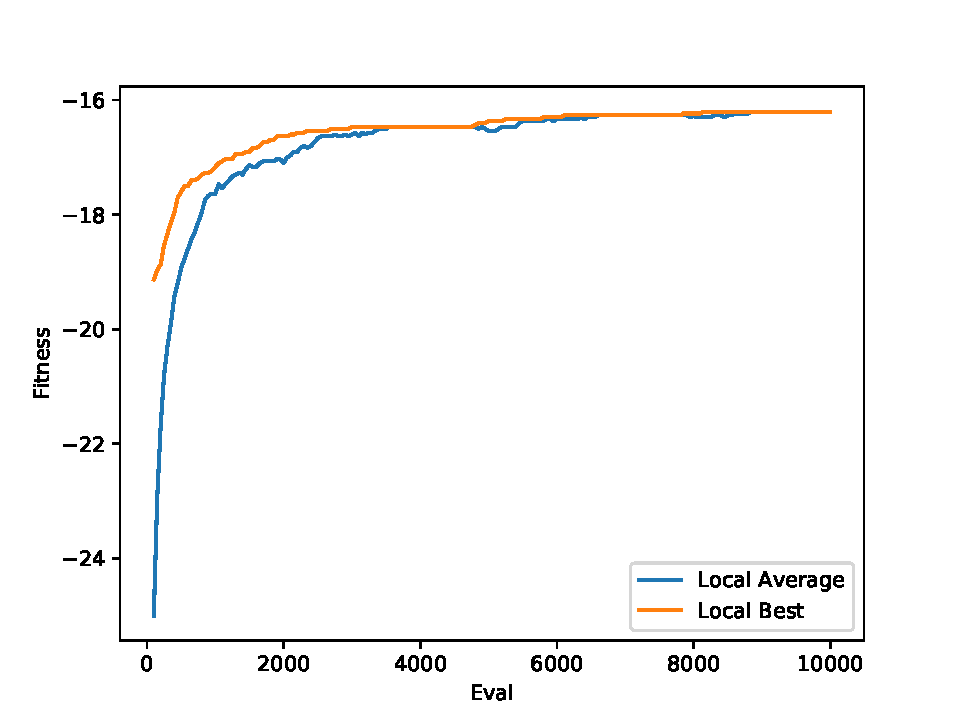
\includegraphics[width=\textwidth]{../graphs/graphs/1003.pdf}
\end{figure}


\begin{table}[!htb]
	\centering
	\caption{Figure \ref{fig:graph_1004} Configuration File}
	\label{tab:graph_1004}
	\begin{tabular}{| c | c |}
		\hline
		Self Adaptive Offspring Count		& True		 \\
		\hline
		Tournament Size For Parent Selection		& 5		 \\
		\hline
		Penalty Coefficient		& 1		 \\
		\hline
		Runs		& 30		 \\
		\hline
		Parent Selection Algorithm		& k-Tournament Selection with replacement		 \\
		\hline
		Self Adaptive Mutation Rate		& False		 \\
		\hline
		Offspring Count		& 50		 \\
		\hline
		Termination Convergence Criterion		& 10000		 \\
		\hline
		Solution File Path		& None		 \\
		\hline
		Mutation Rate		& 0.1		 \\
		\hline
		Recombination Algorithm		& Partially Mapped Crossover		 \\
		\hline
		Random Seed		& 1004		 \\
		\hline
		Mutation Algorithm		& Move		 \\
		\hline
		Tournament Size For Survival Selection		& 5		 \\
		\hline
		Placement Algorithm		& Random		 \\
		\hline
		Population Size		& 100		 \\
		\hline
		Survival Strategy		& Plus		 \\
		\hline
		Search Algorithm		& EA		 \\
		\hline
		Log File Path		& None		 \\
		\hline
		Fitness Evaluations		& 10000		 \\
		\hline
		Survivor Algorithm		& Truncation		 \\
		\hline
		Self Adaptive Penalty Coefficient		& True		 \\
		\hline
	\end{tabular}
\end{table}
\begin{figure}[!htb]
	\caption{Input 1}
	\label{fig:graph_1004}
	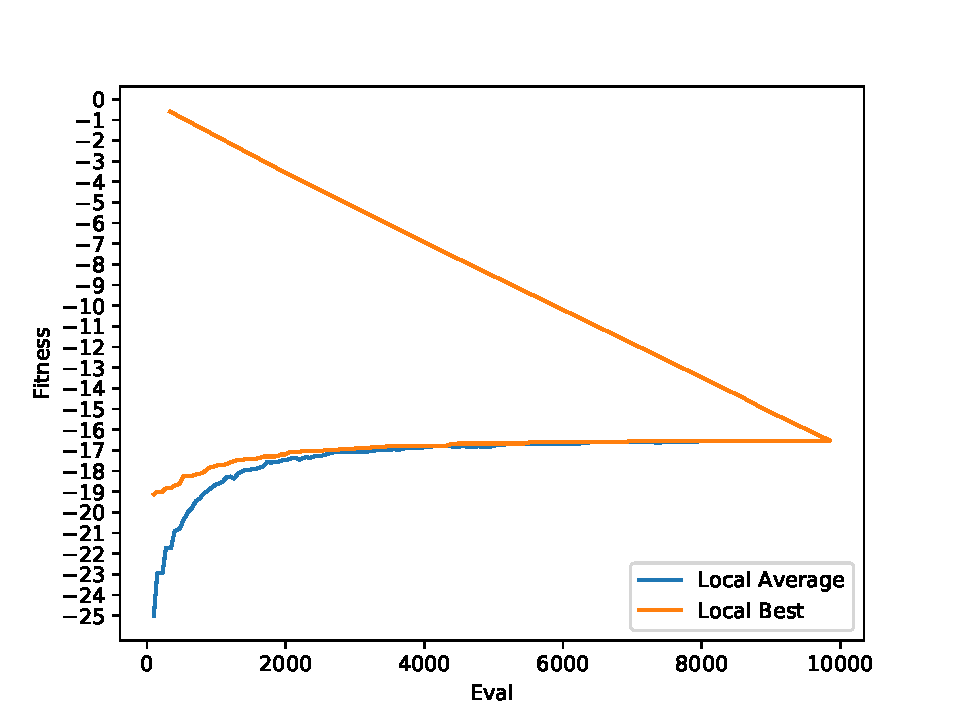
\includegraphics[width=\textwidth]{../graphs/graphs/1004.pdf}
\end{figure}


\begin{table}[!htb]
	\centering
	\caption{Figure \ref{fig:graph_1005} Configuration File}
	\label{tab:graph_1005}
	\begin{tabular}{| c | c |}
		\hline
		Self Adaptive Offspring Count		& False		 \\
		\hline
		Tournament Size For Parent Selection		& 5		 \\
		\hline
		Penalty Coefficient		& 1		 \\
		\hline
		Runs		& 30		 \\
		\hline
		Parent Selection Algorithm		& k-Tournament Selection with replacement		 \\
		\hline
		Self Adaptive Mutation Rate		& True		 \\
		\hline
		Offspring Count		& 50		 \\
		\hline
		Termination Convergence Criterion		& 10000		 \\
		\hline
		Solution File Path		& None		 \\
		\hline
		Mutation Rate		& 0.1		 \\
		\hline
		Recombination Algorithm		& Partially Mapped Crossover		 \\
		\hline
		Random Seed		& 1005		 \\
		\hline
		Mutation Algorithm		& Move		 \\
		\hline
		Tournament Size For Survival Selection		& 5		 \\
		\hline
		Placement Algorithm		& Random		 \\
		\hline
		Population Size		& 100		 \\
		\hline
		Survival Strategy		& Plus		 \\
		\hline
		Search Algorithm		& EA		 \\
		\hline
		Log File Path		& None		 \\
		\hline
		Fitness Evaluations		& 10000		 \\
		\hline
		Survivor Algorithm		& Truncation		 \\
		\hline
		Self Adaptive Penalty Coefficient		& False		 \\
		\hline
	\end{tabular}
\end{table}
\begin{figure}[!htb]
	\caption{Input 1}
	\label{fig:graph_1005}
	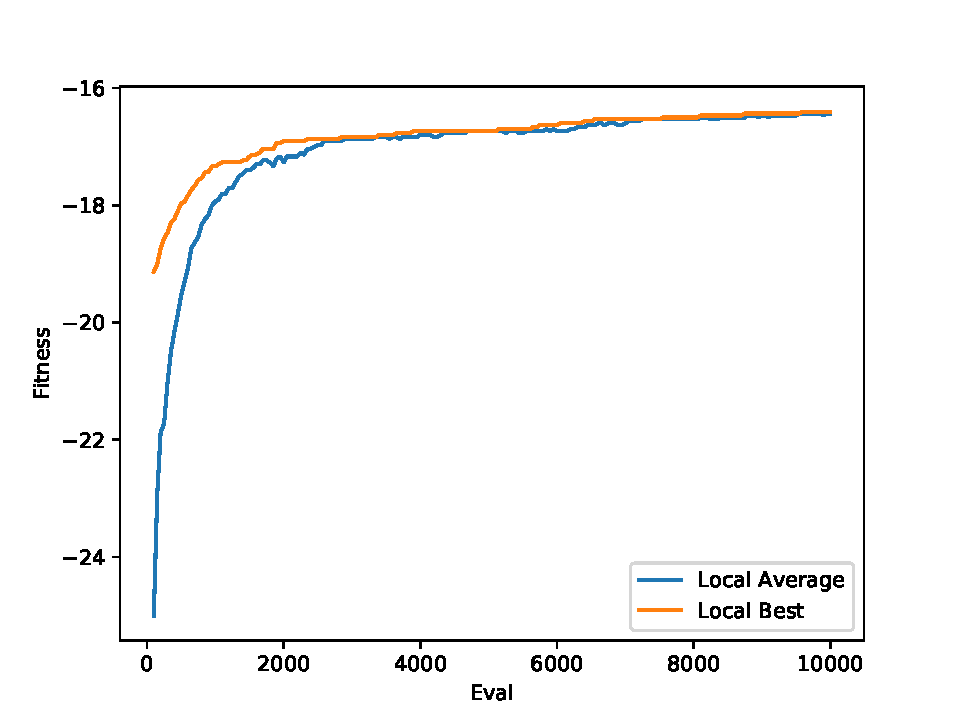
\includegraphics[width=\textwidth]{../graphs/graphs/1005.pdf}
\end{figure}


\begin{table}[!htb]
	\centering
	\caption{Figure \ref{fig:graph_1006} Configuration File}
	\label{tab:graph_1006}
	\begin{tabular}{| c | c |}
		\hline
		Self Adaptive Offspring Count		& True		 \\
		\hline
		Tournament Size For Parent Selection		& 5		 \\
		\hline
		Penalty Coefficient		& 1		 \\
		\hline
		Runs		& 30		 \\
		\hline
		Parent Selection Algorithm		& k-Tournament Selection with replacement		 \\
		\hline
		Self Adaptive Mutation Rate		& True		 \\
		\hline
		Offspring Count		& 50		 \\
		\hline
		Termination Convergence Criterion		& 10000		 \\
		\hline
		Solution File Path		& None		 \\
		\hline
		Mutation Rate		& 0.1		 \\
		\hline
		Recombination Algorithm		& Partially Mapped Crossover		 \\
		\hline
		Random Seed		& 1006		 \\
		\hline
		Mutation Algorithm		& Move		 \\
		\hline
		Tournament Size For Survival Selection		& 5		 \\
		\hline
		Placement Algorithm		& Random		 \\
		\hline
		Population Size		& 100		 \\
		\hline
		Survival Strategy		& Plus		 \\
		\hline
		Search Algorithm		& EA		 \\
		\hline
		Log File Path		& None		 \\
		\hline
		Fitness Evaluations		& 10000		 \\
		\hline
		Survivor Algorithm		& Truncation		 \\
		\hline
		Self Adaptive Penalty Coefficient		& False		 \\
		\hline
	\end{tabular}
\end{table}
\begin{figure}[!htb]
	\caption{Input 1}
	\label{fig:graph_1006}
	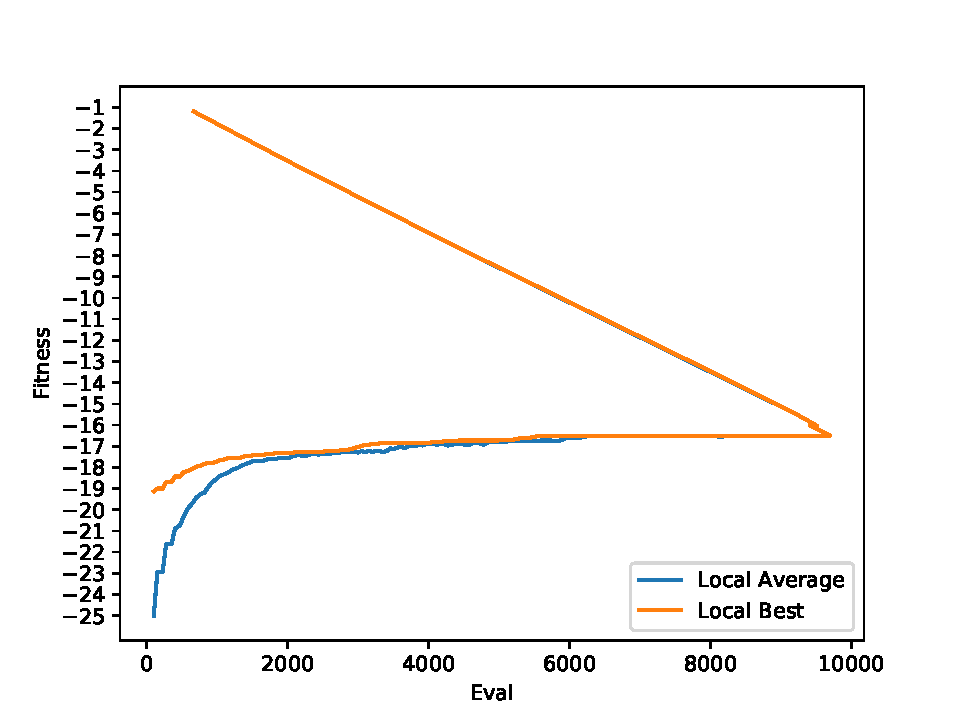
\includegraphics[width=\textwidth]{../graphs/graphs/1006.pdf}
\end{figure}


\begin{table}[!htb]
	\centering
	\caption{Figure \ref{fig:graph_1007} Configuration File}
	\label{tab:graph_1007}
	\begin{tabular}{| c | c |}
		\hline
		Self Adaptive Offspring Count		& False		 \\
		\hline
		Tournament Size For Parent Selection		& 5		 \\
		\hline
		Penalty Coefficient		& 1		 \\
		\hline
		Runs		& 30		 \\
		\hline
		Parent Selection Algorithm		& k-Tournament Selection with replacement		 \\
		\hline
		Self Adaptive Mutation Rate		& True		 \\
		\hline
		Offspring Count		& 50		 \\
		\hline
		Termination Convergence Criterion		& 10000		 \\
		\hline
		Solution File Path		& None		 \\
		\hline
		Mutation Rate		& 0.1		 \\
		\hline
		Recombination Algorithm		& Partially Mapped Crossover		 \\
		\hline
		Random Seed		& 1007		 \\
		\hline
		Mutation Algorithm		& Move		 \\
		\hline
		Tournament Size For Survival Selection		& 5		 \\
		\hline
		Placement Algorithm		& Random		 \\
		\hline
		Population Size		& 100		 \\
		\hline
		Survival Strategy		& Plus		 \\
		\hline
		Search Algorithm		& EA		 \\
		\hline
		Log File Path		& None		 \\
		\hline
		Fitness Evaluations		& 10000		 \\
		\hline
		Survivor Algorithm		& Truncation		 \\
		\hline
		Self Adaptive Penalty Coefficient		& True		 \\
		\hline
	\end{tabular}
\end{table}
\begin{figure}[!htb]
	\caption{Input 1}
	\label{fig:graph_1007}
	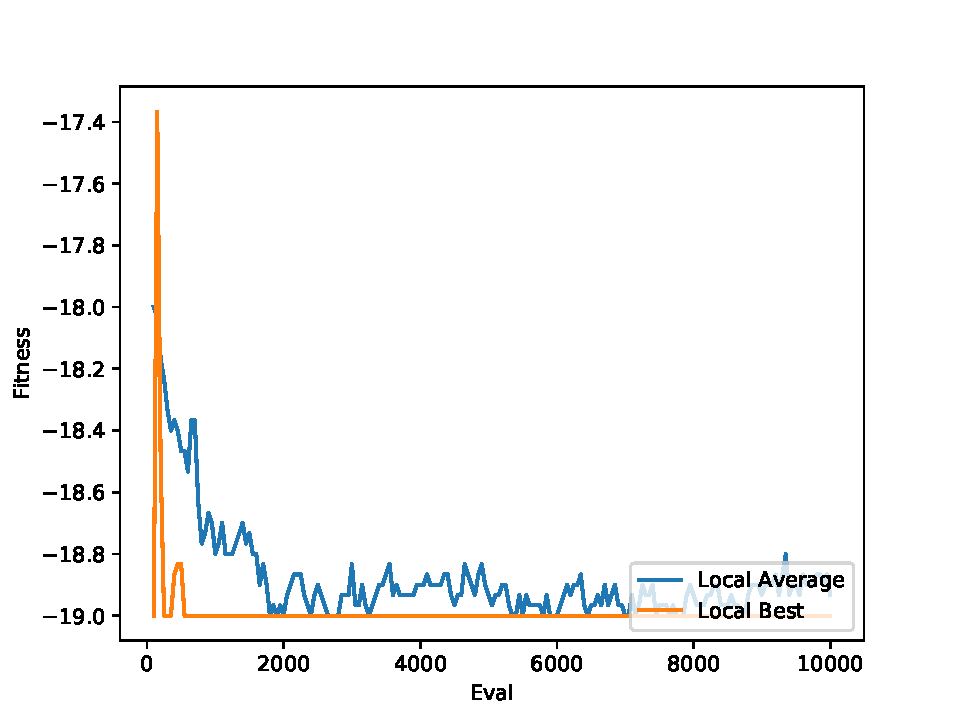
\includegraphics[width=\textwidth]{../graphs/graphs/1007.pdf}
\end{figure}


\begin{table}[!htb]
	\centering
	\caption{Figure \ref{fig:graph_1008} Configuration File}
	\label{tab:graph_1008}
	\begin{tabular}{| c | c |}
		\hline
		Self Adaptive Offspring Count		& True		 \\
		\hline
		Tournament Size For Parent Selection		& 5		 \\
		\hline
		Penalty Coefficient		& 1		 \\
		\hline
		Runs		& 30		 \\
		\hline
		Parent Selection Algorithm		& k-Tournament Selection with replacement		 \\
		\hline
		Self Adaptive Mutation Rate		& True		 \\
		\hline
		Offspring Count		& 50		 \\
		\hline
		Termination Convergence Criterion		& 10000		 \\
		\hline
		Solution File Path		& None		 \\
		\hline
		Mutation Rate		& 0.1		 \\
		\hline
		Recombination Algorithm		& Partially Mapped Crossover		 \\
		\hline
		Random Seed		& 1008		 \\
		\hline
		Mutation Algorithm		& Move		 \\
		\hline
		Tournament Size For Survival Selection		& 5		 \\
		\hline
		Placement Algorithm		& Random		 \\
		\hline
		Population Size		& 100		 \\
		\hline
		Survival Strategy		& Plus		 \\
		\hline
		Search Algorithm		& EA		 \\
		\hline
		Log File Path		& None		 \\
		\hline
		Fitness Evaluations		& 10000		 \\
		\hline
		Survivor Algorithm		& Truncation		 \\
		\hline
		Self Adaptive Penalty Coefficient		& True		 \\
		\hline
	\end{tabular}
\end{table}
\begin{figure}[!htb]
	\caption{Input 1}
	\label{fig:graph_1008}
	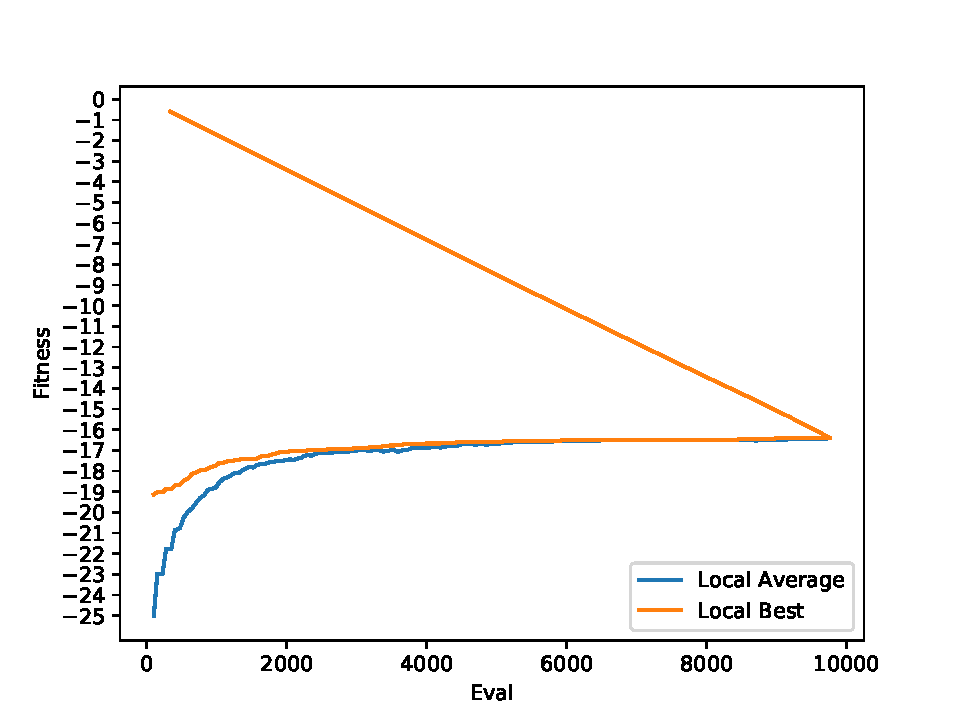
\includegraphics[width=\textwidth]{../graphs/graphs/1008.pdf}
\end{figure}


\begin{table}[!htb]
	\centering
	\caption{Figure \ref{fig:graph_1009} Configuration File}
	\label{tab:graph_1009}
	\begin{tabular}{| c | c |}
		\hline
		Self Adaptive Offspring Count		& False		 \\
		\hline
		Tournament Size For Parent Selection		& 5		 \\
		\hline
		Penalty Coefficient		& 1		 \\
		\hline
		Runs		& 30		 \\
		\hline
		Parent Selection Algorithm		& k-Tournament Selection with replacement		 \\
		\hline
		Self Adaptive Mutation Rate		& False		 \\
		\hline
		Offspring Count		& 50		 \\
		\hline
		Termination Convergence Criterion		& 10000		 \\
		\hline
		Solution File Path		& None		 \\
		\hline
		Mutation Rate		& 0.1		 \\
		\hline
		Recombination Algorithm		& Partially Mapped Crossover		 \\
		\hline
		Random Seed		& 1009		 \\
		\hline
		Mutation Algorithm		& Move		 \\
		\hline
		Tournament Size For Survival Selection		& 5		 \\
		\hline
		Placement Algorithm		& Random with Repair		 \\
		\hline
		Population Size		& 100		 \\
		\hline
		Survival Strategy		& Plus		 \\
		\hline
		Search Algorithm		& EA		 \\
		\hline
		Log File Path		& None		 \\
		\hline
		Fitness Evaluations		& 10000		 \\
		\hline
		Survivor Algorithm		& Truncation		 \\
		\hline
		Self Adaptive Penalty Coefficient		& False		 \\
		\hline
	\end{tabular}
\end{table}
\begin{figure}[!htb]
	\caption{Input 1}
	\label{fig:graph_1009}
	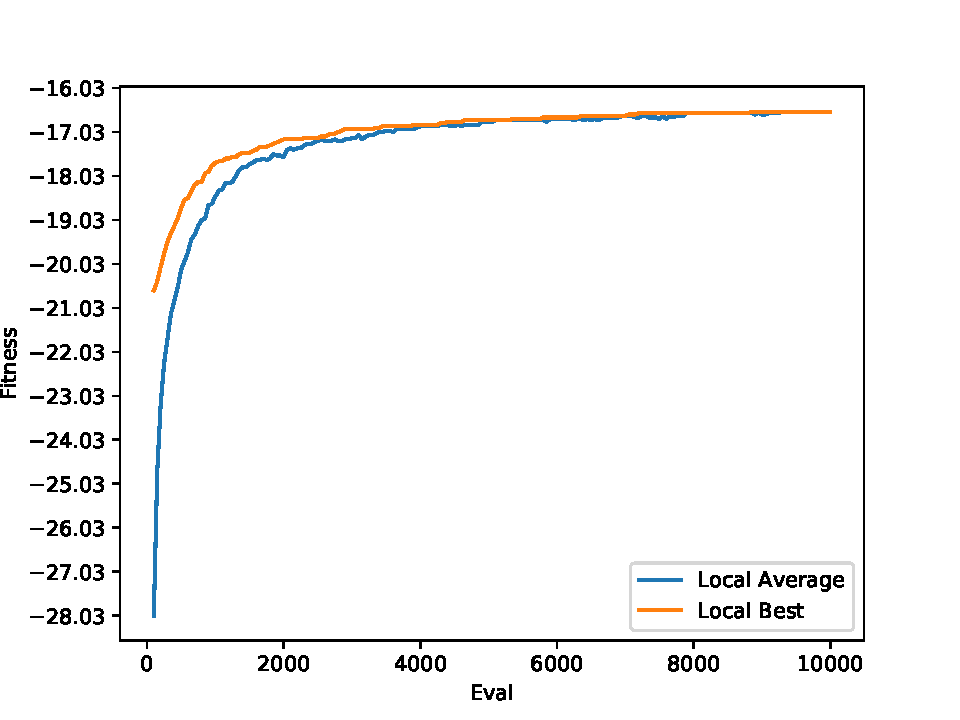
\includegraphics[width=\textwidth]{../graphs/graphs/1009.pdf}
\end{figure}


\begin{table}[!htb]
	\centering
	\caption{Figure \ref{fig:graph_1010} Configuration File}
	\label{tab:graph_1010}
	\begin{tabular}{| c | c |}
		\hline
		Self Adaptive Offspring Count		& True		 \\
		\hline
		Tournament Size For Parent Selection		& 5		 \\
		\hline
		Penalty Coefficient		& 1		 \\
		\hline
		Runs		& 30		 \\
		\hline
		Parent Selection Algorithm		& k-Tournament Selection with replacement		 \\
		\hline
		Self Adaptive Mutation Rate		& False		 \\
		\hline
		Offspring Count		& 50		 \\
		\hline
		Termination Convergence Criterion		& 10000		 \\
		\hline
		Solution File Path		& None		 \\
		\hline
		Mutation Rate		& 0.1		 \\
		\hline
		Recombination Algorithm		& Partially Mapped Crossover		 \\
		\hline
		Random Seed		& 1010		 \\
		\hline
		Mutation Algorithm		& Move		 \\
		\hline
		Tournament Size For Survival Selection		& 5		 \\
		\hline
		Placement Algorithm		& Random with Repair		 \\
		\hline
		Population Size		& 100		 \\
		\hline
		Survival Strategy		& Plus		 \\
		\hline
		Search Algorithm		& EA		 \\
		\hline
		Log File Path		& None		 \\
		\hline
		Fitness Evaluations		& 10000		 \\
		\hline
		Survivor Algorithm		& Truncation		 \\
		\hline
		Self Adaptive Penalty Coefficient		& False		 \\
		\hline
	\end{tabular}
\end{table}
\begin{figure}[!htb]
	\caption{Input 1}
	\label{fig:graph_1010}
	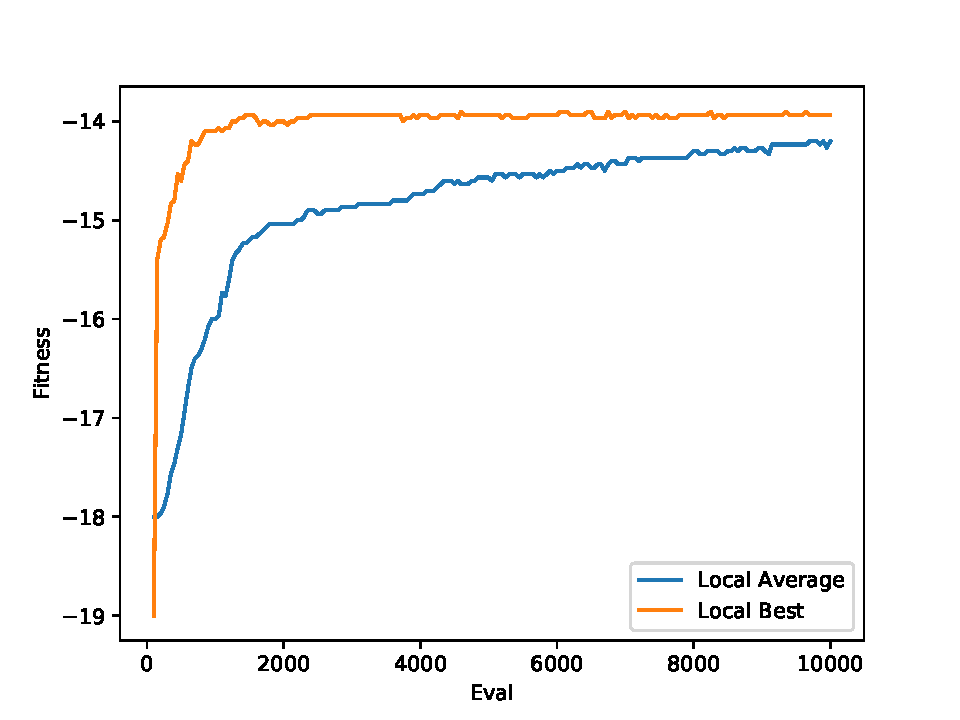
\includegraphics[width=\textwidth]{../graphs/graphs/1010.pdf}
\end{figure}


\clearpage
\begin{table}[!htb]
	\centering
	\caption{Figure \ref{fig:graph_1011} Configuration File}
	\label{tab:graph_1011}
	\begin{tabular}{| c | c |}
		\hline
		Self Adaptive Offspring Count		& False		 \\
		\hline
		Tournament Size For Parent Selection		& 5		 \\
		\hline
		Penalty Coefficient		& 1		 \\
		\hline
		Runs		& 30		 \\
		\hline
		Parent Selection Algorithm		& k-Tournament Selection with replacement		 \\
		\hline
		Self Adaptive Mutation Rate		& False		 \\
		\hline
		Offspring Count		& 50		 \\
		\hline
		Termination Convergence Criterion		& 10000		 \\
		\hline
		Solution File Path		& None		 \\
		\hline
		Mutation Rate		& 0.1		 \\
		\hline
		Recombination Algorithm		& Partially Mapped Crossover		 \\
		\hline
		Random Seed		& 1011		 \\
		\hline
		Mutation Algorithm		& Move		 \\
		\hline
		Tournament Size For Survival Selection		& 5		 \\
		\hline
		Placement Algorithm		& Random with Repair		 \\
		\hline
		Population Size		& 100		 \\
		\hline
		Survival Strategy		& Plus		 \\
		\hline
		Search Algorithm		& EA		 \\
		\hline
		Log File Path		& None		 \\
		\hline
		Fitness Evaluations		& 10000		 \\
		\hline
		Survivor Algorithm		& Truncation		 \\
		\hline
		Self Adaptive Penalty Coefficient		& True		 \\
		\hline
	\end{tabular}
\end{table}
\begin{figure}[!htb]
	\caption{Input 1}
	\label{fig:graph_1011}
	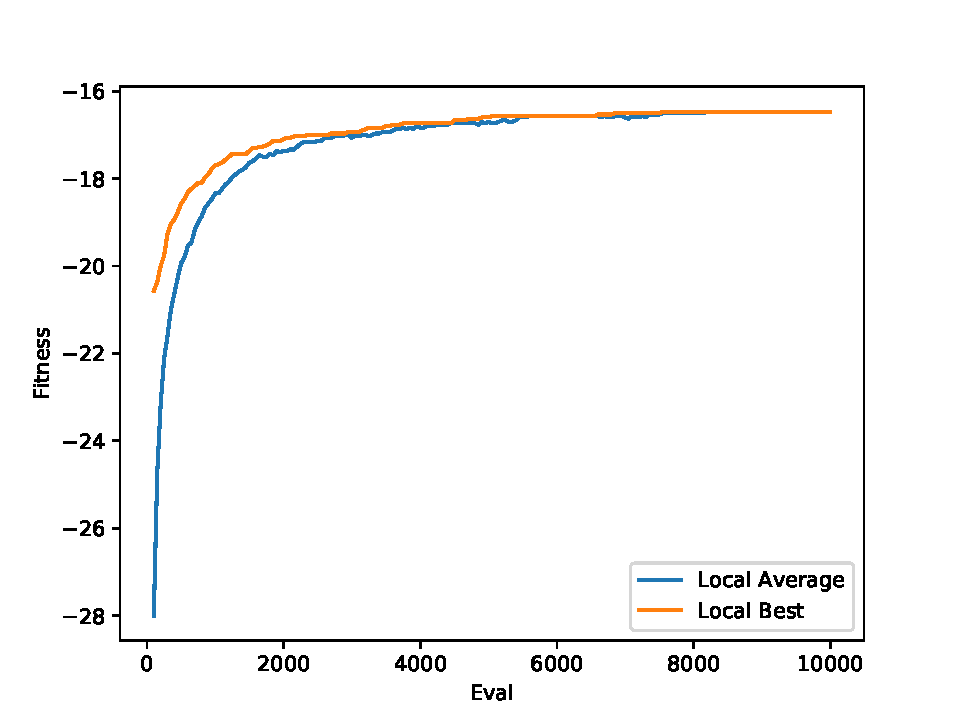
\includegraphics[width=\textwidth]{../graphs/graphs/1011.pdf}
\end{figure}


\begin{table}[!htb]
	\centering
	\caption{Figure \ref{fig:graph_1012} Configuration File}
	\label{tab:graph_1012}
	\begin{tabular}{| c | c |}
		\hline
		Self Adaptive Offspring Count		& True		 \\
		\hline
		Tournament Size For Parent Selection		& 5		 \\
		\hline
		Penalty Coefficient		& 1		 \\
		\hline
		Runs		& 30		 \\
		\hline
		Parent Selection Algorithm		& k-Tournament Selection with replacement		 \\
		\hline
		Self Adaptive Mutation Rate		& False		 \\
		\hline
		Offspring Count		& 50		 \\
		\hline
		Termination Convergence Criterion		& 10000		 \\
		\hline
		Solution File Path		& None		 \\
		\hline
		Mutation Rate		& 0.1		 \\
		\hline
		Recombination Algorithm		& Partially Mapped Crossover		 \\
		\hline
		Random Seed		& 1012		 \\
		\hline
		Mutation Algorithm		& Move		 \\
		\hline
		Tournament Size For Survival Selection		& 5		 \\
		\hline
		Placement Algorithm		& Random with Repair		 \\
		\hline
		Population Size		& 100		 \\
		\hline
		Survival Strategy		& Plus		 \\
		\hline
		Search Algorithm		& EA		 \\
		\hline
		Log File Path		& None		 \\
		\hline
		Fitness Evaluations		& 10000		 \\
		\hline
		Survivor Algorithm		& Truncation		 \\
		\hline
		Self Adaptive Penalty Coefficient		& True		 \\
		\hline
	\end{tabular}
\end{table}
\begin{figure}[!htb]
	\caption{Input 1}
	\label{fig:graph_1012}
	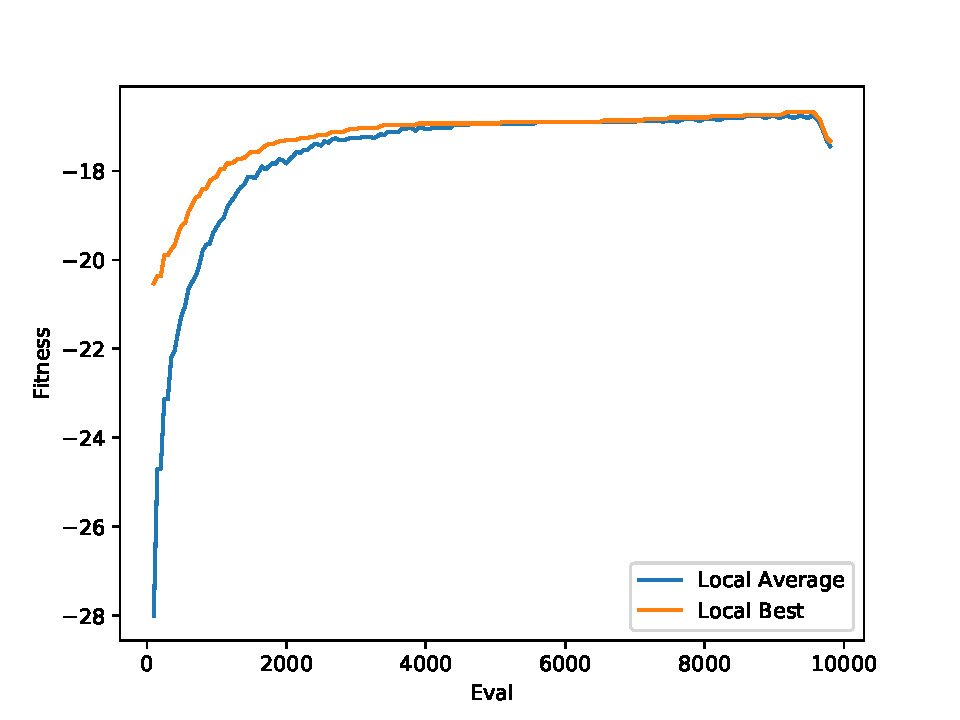
\includegraphics[width=\textwidth]{../graphs/graphs/1012.pdf}
\end{figure}


\begin{table}[!htb]
	\centering
	\caption{Figure \ref{fig:graph_1013} Configuration File}
	\label{tab:graph_1013}
	\begin{tabular}{| c | c |}
		\hline
		Self Adaptive Offspring Count		& False		 \\
		\hline
		Tournament Size For Parent Selection		& 5		 \\
		\hline
		Penalty Coefficient		& 1		 \\
		\hline
		Runs		& 30		 \\
		\hline
		Parent Selection Algorithm		& k-Tournament Selection with replacement		 \\
		\hline
		Self Adaptive Mutation Rate		& True		 \\
		\hline
		Offspring Count		& 50		 \\
		\hline
		Termination Convergence Criterion		& 10000		 \\
		\hline
		Solution File Path		& None		 \\
		\hline
		Mutation Rate		& 0.1		 \\
		\hline
		Recombination Algorithm		& Partially Mapped Crossover		 \\
		\hline
		Random Seed		& 1013		 \\
		\hline
		Mutation Algorithm		& Move		 \\
		\hline
		Tournament Size For Survival Selection		& 5		 \\
		\hline
		Placement Algorithm		& Random with Repair		 \\
		\hline
		Population Size		& 100		 \\
		\hline
		Survival Strategy		& Plus		 \\
		\hline
		Search Algorithm		& EA		 \\
		\hline
		Log File Path		& None		 \\
		\hline
		Fitness Evaluations		& 10000		 \\
		\hline
		Survivor Algorithm		& Truncation		 \\
		\hline
		Self Adaptive Penalty Coefficient		& False		 \\
		\hline
	\end{tabular}
\end{table}
\begin{figure}[!htb]
	\caption{Input 1}
	\label{fig:graph_1013}
	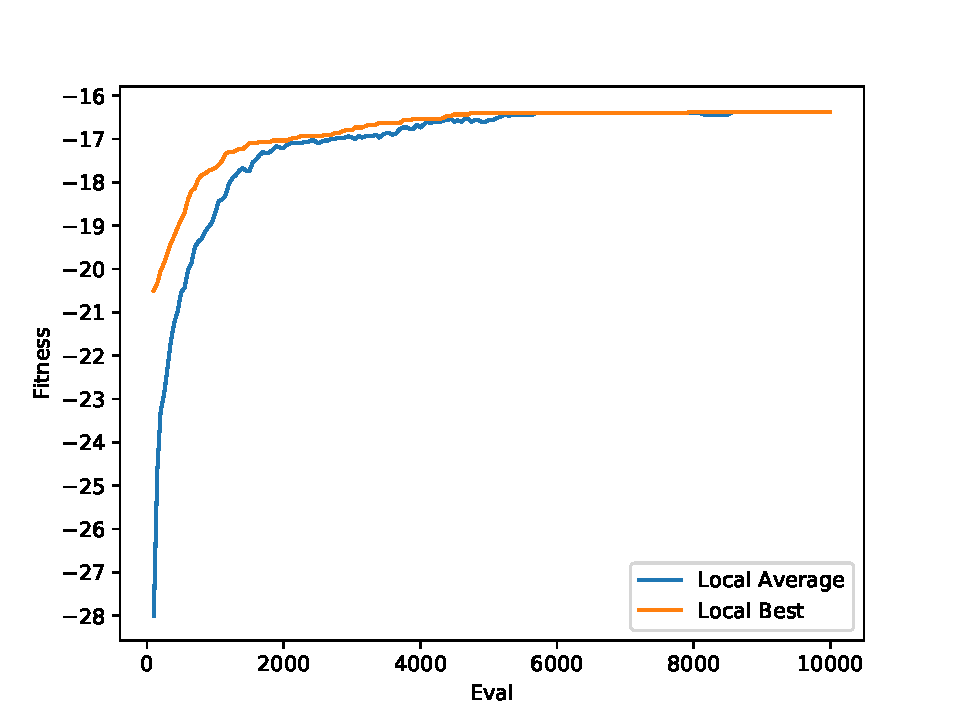
\includegraphics[width=\textwidth]{../graphs/graphs/1013.pdf}
\end{figure}


\begin{table}[!htb]
	\centering
	\caption{Figure \ref{fig:graph_1014} Configuration File}
	\label{tab:graph_1014}
	\begin{tabular}{| c | c |}
		\hline
		Self Adaptive Offspring Count		& True		 \\
		\hline
		Tournament Size For Parent Selection		& 5		 \\
		\hline
		Penalty Coefficient		& 1		 \\
		\hline
		Runs		& 30		 \\
		\hline
		Parent Selection Algorithm		& k-Tournament Selection with replacement		 \\
		\hline
		Self Adaptive Mutation Rate		& True		 \\
		\hline
		Offspring Count		& 50		 \\
		\hline
		Termination Convergence Criterion		& 10000		 \\
		\hline
		Solution File Path		& None		 \\
		\hline
		Mutation Rate		& 0.1		 \\
		\hline
		Recombination Algorithm		& Partially Mapped Crossover		 \\
		\hline
		Random Seed		& 1014		 \\
		\hline
		Mutation Algorithm		& Move		 \\
		\hline
		Tournament Size For Survival Selection		& 5		 \\
		\hline
		Placement Algorithm		& Random with Repair		 \\
		\hline
		Population Size		& 100		 \\
		\hline
		Survival Strategy		& Plus		 \\
		\hline
		Search Algorithm		& EA		 \\
		\hline
		Log File Path		& None		 \\
		\hline
		Fitness Evaluations		& 10000		 \\
		\hline
		Survivor Algorithm		& Truncation		 \\
		\hline
		Self Adaptive Penalty Coefficient		& False		 \\
		\hline
	\end{tabular}
\end{table}
\begin{figure}[!htb]
	\caption{Input 1}
	\label{fig:graph_1014}
	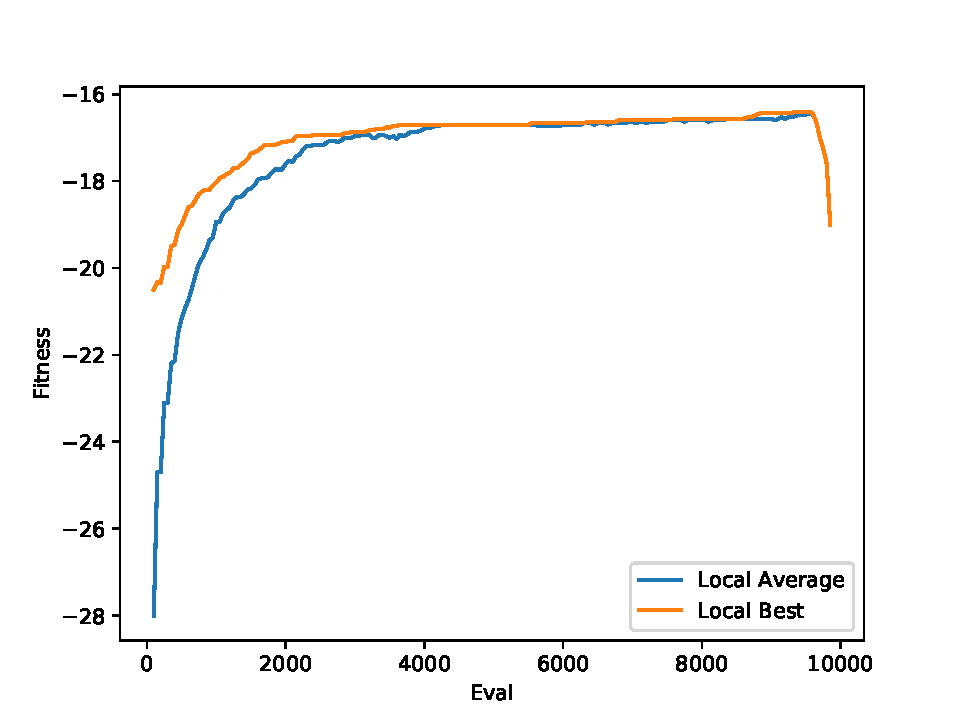
\includegraphics[width=\textwidth]{../graphs/graphs/1014.pdf}
\end{figure}


\begin{table}[!htb]
	\centering
	\caption{Figure \ref{fig:graph_1015} Configuration File}
	\label{tab:graph_1015}
	\begin{tabular}{| c | c |}
		\hline
		Self Adaptive Offspring Count		& False		 \\
		\hline
		Tournament Size For Parent Selection		& 5		 \\
		\hline
		Penalty Coefficient		& 1		 \\
		\hline
		Runs		& 30		 \\
		\hline
		Parent Selection Algorithm		& k-Tournament Selection with replacement		 \\
		\hline
		Self Adaptive Mutation Rate		& True		 \\
		\hline
		Offspring Count		& 50		 \\
		\hline
		Termination Convergence Criterion		& 10000		 \\
		\hline
		Solution File Path		& None		 \\
		\hline
		Mutation Rate		& 0.1		 \\
		\hline
		Recombination Algorithm		& Partially Mapped Crossover		 \\
		\hline
		Random Seed		& 1015		 \\
		\hline
		Mutation Algorithm		& Move		 \\
		\hline
		Tournament Size For Survival Selection		& 5		 \\
		\hline
		Placement Algorithm		& Random with Repair		 \\
		\hline
		Population Size		& 100		 \\
		\hline
		Survival Strategy		& Plus		 \\
		\hline
		Search Algorithm		& EA		 \\
		\hline
		Log File Path		& None		 \\
		\hline
		Fitness Evaluations		& 10000		 \\
		\hline
		Survivor Algorithm		& Truncation		 \\
		\hline
		Self Adaptive Penalty Coefficient		& True		 \\
		\hline
	\end{tabular}
\end{table}
\begin{figure}[!htb]
	\caption{Input 1}
	\label{fig:graph_1015}
	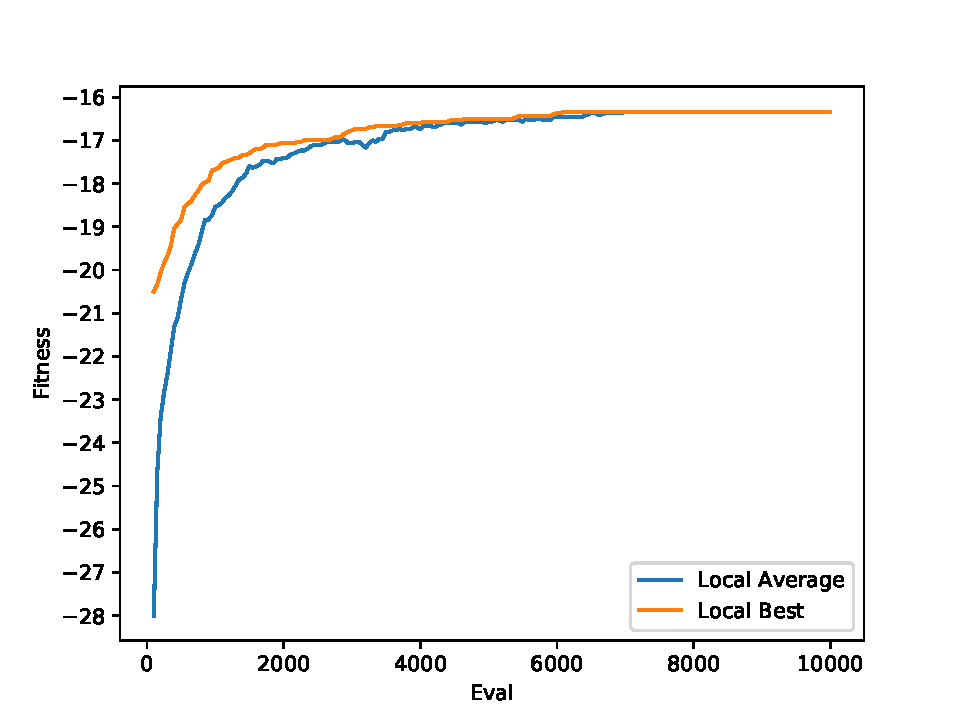
\includegraphics[width=\textwidth]{../graphs/graphs/1015.pdf}
\end{figure}


\begin{table}[!htb]
	\centering
	\caption{Figure \ref{fig:graph_1016} Configuration File}
	\label{tab:graph_1016}
	\begin{tabular}{| c | c |}
		\hline
		Self Adaptive Offspring Count		& True		 \\
		\hline
		Tournament Size For Parent Selection		& 5		 \\
		\hline
		Penalty Coefficient		& 1		 \\
		\hline
		Runs		& 30		 \\
		\hline
		Parent Selection Algorithm		& k-Tournament Selection with replacement		 \\
		\hline
		Self Adaptive Mutation Rate		& True		 \\
		\hline
		Offspring Count		& 50		 \\
		\hline
		Termination Convergence Criterion		& 10000		 \\
		\hline
		Solution File Path		& None		 \\
		\hline
		Mutation Rate		& 0.1		 \\
		\hline
		Recombination Algorithm		& Partially Mapped Crossover		 \\
		\hline
		Random Seed		& 1016		 \\
		\hline
		Mutation Algorithm		& Move		 \\
		\hline
		Tournament Size For Survival Selection		& 5		 \\
		\hline
		Placement Algorithm		& Random with Repair		 \\
		\hline
		Population Size		& 100		 \\
		\hline
		Survival Strategy		& Plus		 \\
		\hline
		Search Algorithm		& EA		 \\
		\hline
		Log File Path		& None		 \\
		\hline
		Fitness Evaluations		& 10000		 \\
		\hline
		Survivor Algorithm		& Truncation		 \\
		\hline
		Self Adaptive Penalty Coefficient		& True		 \\
		\hline
	\end{tabular}
\end{table}
\begin{figure}[!htb]
	\caption{Input 1}
	\label{fig:graph_1016}
	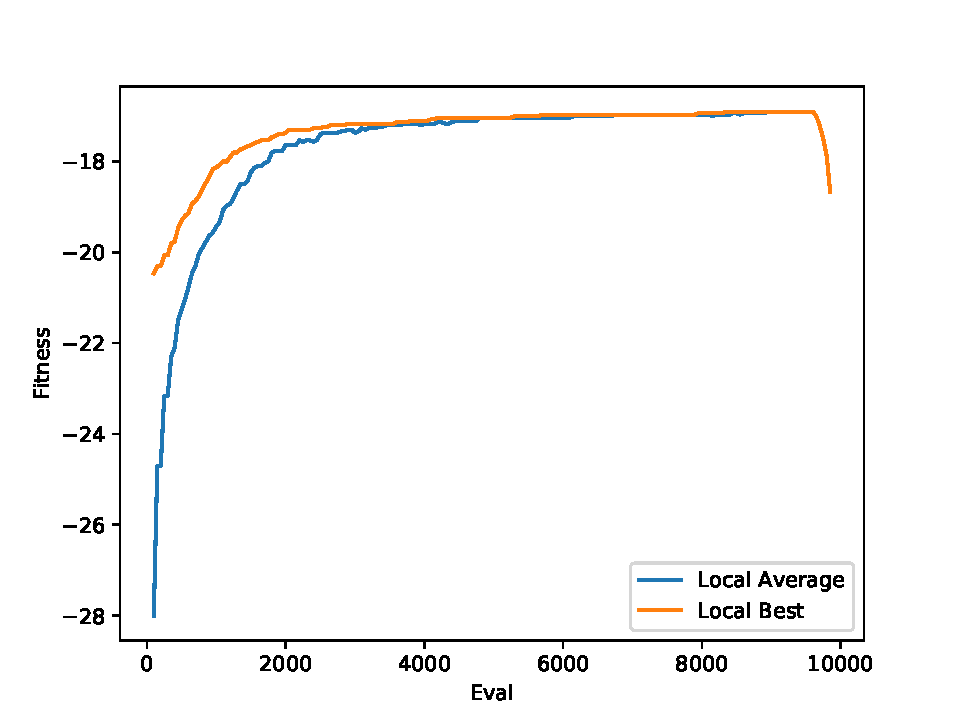
\includegraphics[width=\textwidth]{../graphs/graphs/1016.pdf}
\end{figure}


\begin{table}[!htb]
	\centering
	\caption{Figure \ref{fig:graph_1017} Configuration File}
	\label{tab:graph_1017}
	\begin{tabular}{| c | c |}
		\hline
		Self Adaptive Offspring Count		& False		 \\
		\hline
		Tournament Size For Parent Selection		& 5		 \\
		\hline
		Penalty Coefficient		& 1		 \\
		\hline
		Runs		& 30		 \\
		\hline
		Parent Selection Algorithm		& k-Tournament Selection with replacement		 \\
		\hline
		Self Adaptive Mutation Rate		& False		 \\
		\hline
		Offspring Count		& 50		 \\
		\hline
		Termination Convergence Criterion		& 10000		 \\
		\hline
		Solution File Path		& None		 \\
		\hline
		Mutation Rate		& 0.1		 \\
		\hline
		Recombination Algorithm		& Partially Mapped Crossover		 \\
		\hline
		Random Seed		& 1017		 \\
		\hline
		Mutation Algorithm		& Move		 \\
		\hline
		Tournament Size For Survival Selection		& 5		 \\
		\hline
		Placement Algorithm		& Random with Penalty		 \\
		\hline
		Population Size		& 100		 \\
		\hline
		Survival Strategy		& Plus		 \\
		\hline
		Search Algorithm		& EA		 \\
		\hline
		Log File Path		& None		 \\
		\hline
		Fitness Evaluations		& 10000		 \\
		\hline
		Survivor Algorithm		& Truncation		 \\
		\hline
		Self Adaptive Penalty Coefficient		& False		 \\
		\hline
	\end{tabular}
\end{table}
\begin{figure}[!htb]
	\caption{Input 1}
	\label{fig:graph_1017}
	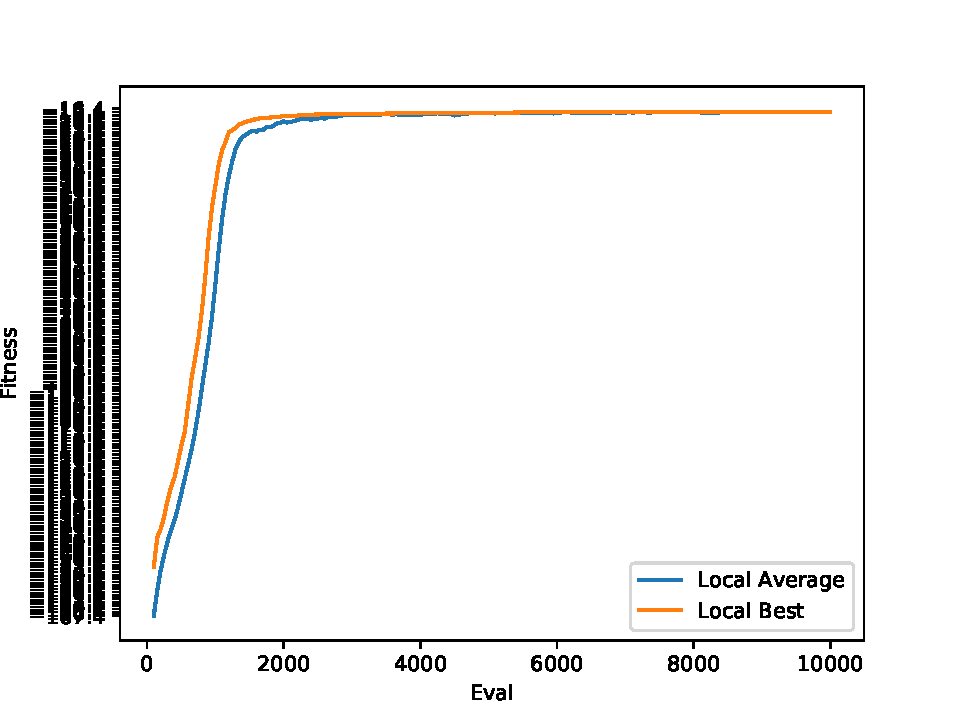
\includegraphics[width=\textwidth]{../graphs/graphs/1017.pdf}
\end{figure}


\begin{table}[!htb]
	\centering
	\caption{Figure \ref{fig:graph_1018} Configuration File}
	\label{tab:graph_1018}
	\begin{tabular}{| c | c |}
		\hline
		Self Adaptive Offspring Count		& True		 \\
		\hline
		Tournament Size For Parent Selection		& 5		 \\
		\hline
		Penalty Coefficient		& 1		 \\
		\hline
		Runs		& 30		 \\
		\hline
		Parent Selection Algorithm		& k-Tournament Selection with replacement		 \\
		\hline
		Self Adaptive Mutation Rate		& False		 \\
		\hline
		Offspring Count		& 50		 \\
		\hline
		Termination Convergence Criterion		& 10000		 \\
		\hline
		Solution File Path		& None		 \\
		\hline
		Mutation Rate		& 0.1		 \\
		\hline
		Recombination Algorithm		& Partially Mapped Crossover		 \\
		\hline
		Random Seed		& 1018		 \\
		\hline
		Mutation Algorithm		& Move		 \\
		\hline
		Tournament Size For Survival Selection		& 5		 \\
		\hline
		Placement Algorithm		& Random with Penalty		 \\
		\hline
		Population Size		& 100		 \\
		\hline
		Survival Strategy		& Plus		 \\
		\hline
		Search Algorithm		& EA		 \\
		\hline
		Log File Path		& None		 \\
		\hline
		Fitness Evaluations		& 10000		 \\
		\hline
		Survivor Algorithm		& Truncation		 \\
		\hline
		Self Adaptive Penalty Coefficient		& False		 \\
		\hline
	\end{tabular}
\end{table}
\begin{figure}[!htb]
	\caption{Input 1}
	\label{fig:graph_1018}
	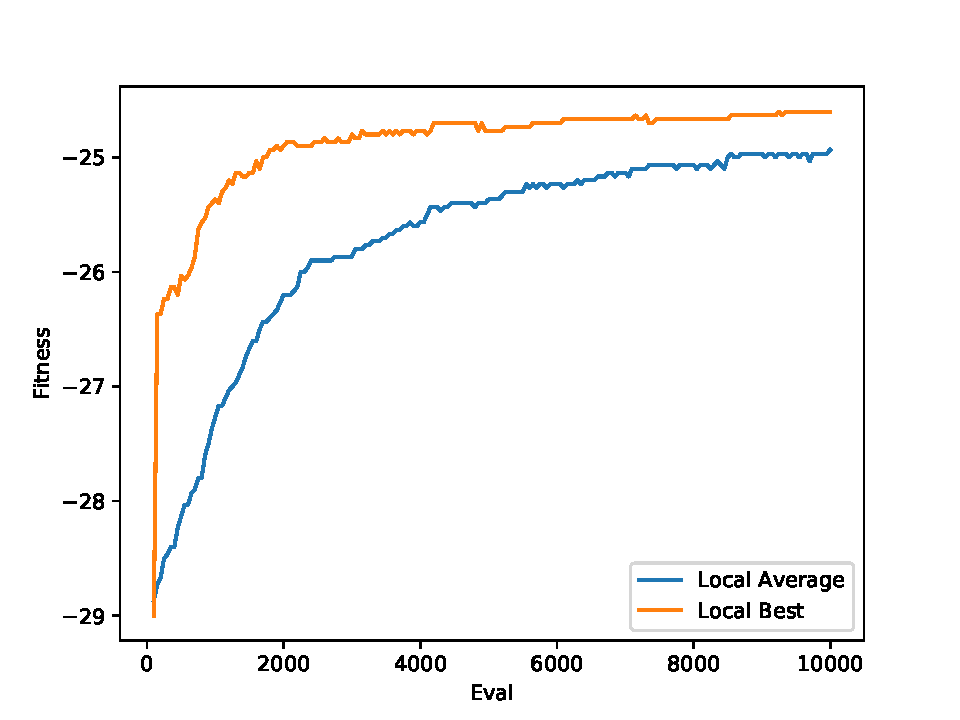
\includegraphics[width=\textwidth]{../graphs/graphs/1018.pdf}
\end{figure}


\begin{table}[!htb]
	\centering
	\caption{Figure \ref{fig:graph_1019} Configuration File}
	\label{tab:graph_1019}
	\begin{tabular}{| c | c |}
		\hline
		Self Adaptive Offspring Count		& False		 \\
		\hline
		Tournament Size For Parent Selection		& 5		 \\
		\hline
		Penalty Coefficient		& 1		 \\
		\hline
		Runs		& 30		 \\
		\hline
		Parent Selection Algorithm		& k-Tournament Selection with replacement		 \\
		\hline
		Self Adaptive Mutation Rate		& False		 \\
		\hline
		Offspring Count		& 50		 \\
		\hline
		Termination Convergence Criterion		& 10000		 \\
		\hline
		Solution File Path		& None		 \\
		\hline
		Mutation Rate		& 0.1		 \\
		\hline
		Recombination Algorithm		& Partially Mapped Crossover		 \\
		\hline
		Random Seed		& 1019		 \\
		\hline
		Mutation Algorithm		& Move		 \\
		\hline
		Tournament Size For Survival Selection		& 5		 \\
		\hline
		Placement Algorithm		& Random with Penalty		 \\
		\hline
		Population Size		& 100		 \\
		\hline
		Survival Strategy		& Plus		 \\
		\hline
		Search Algorithm		& EA		 \\
		\hline
		Log File Path		& None		 \\
		\hline
		Fitness Evaluations		& 10000		 \\
		\hline
		Survivor Algorithm		& Truncation		 \\
		\hline
		Self Adaptive Penalty Coefficient		& True		 \\
		\hline
	\end{tabular}
\end{table}
\begin{figure}[!htb]
	\caption{Input 1}
	\label{fig:graph_1019}
	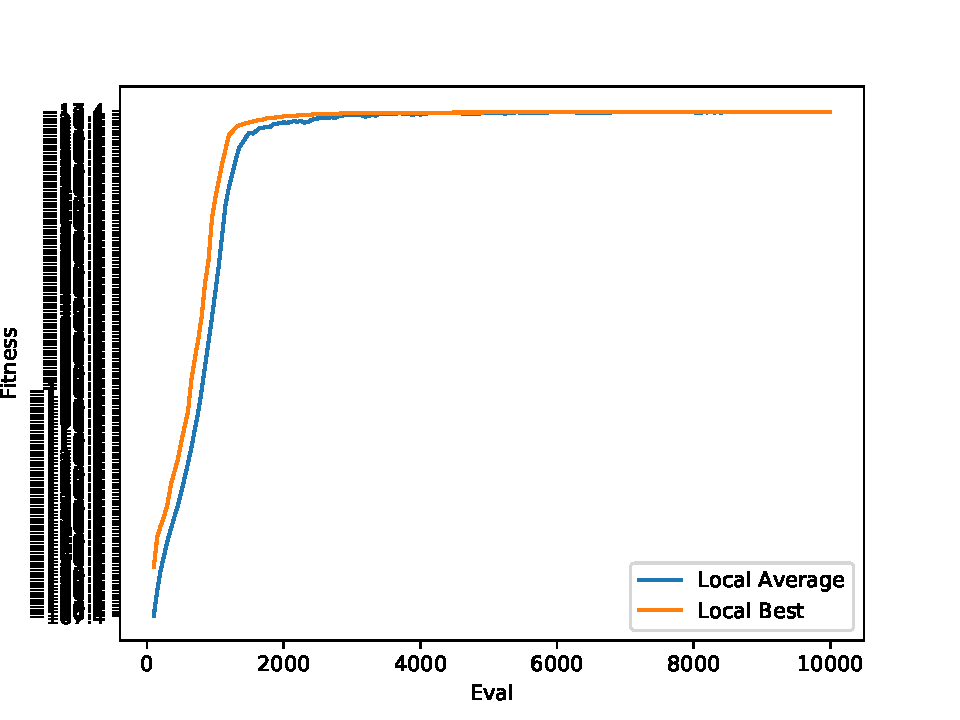
\includegraphics[width=\textwidth]{../graphs/graphs/1019.pdf}
\end{figure}


\begin{table}[!htb]
	\centering
	\caption{Figure \ref{fig:graph_1020} Configuration File}
	\label{tab:graph_1020}
	\begin{tabular}{| c | c |}
		\hline
		Self Adaptive Offspring Count		& True		 \\
		\hline
		Tournament Size For Parent Selection		& 5		 \\
		\hline
		Penalty Coefficient		& 1		 \\
		\hline
		Runs		& 30		 \\
		\hline
		Parent Selection Algorithm		& k-Tournament Selection with replacement		 \\
		\hline
		Self Adaptive Mutation Rate		& False		 \\
		\hline
		Offspring Count		& 50		 \\
		\hline
		Termination Convergence Criterion		& 10000		 \\
		\hline
		Solution File Path		& None		 \\
		\hline
		Mutation Rate		& 0.1		 \\
		\hline
		Recombination Algorithm		& Partially Mapped Crossover		 \\
		\hline
		Random Seed		& 1020		 \\
		\hline
		Mutation Algorithm		& Move		 \\
		\hline
		Tournament Size For Survival Selection		& 5		 \\
		\hline
		Placement Algorithm		& Random with Penalty		 \\
		\hline
		Population Size		& 100		 \\
		\hline
		Survival Strategy		& Plus		 \\
		\hline
		Search Algorithm		& EA		 \\
		\hline
		Log File Path		& None		 \\
		\hline
		Fitness Evaluations		& 10000		 \\
		\hline
		Survivor Algorithm		& Truncation		 \\
		\hline
		Self Adaptive Penalty Coefficient		& True		 \\
		\hline
	\end{tabular}
\end{table}
\begin{figure}[!htb]
	\caption{Input 1}
	\label{fig:graph_1020}
	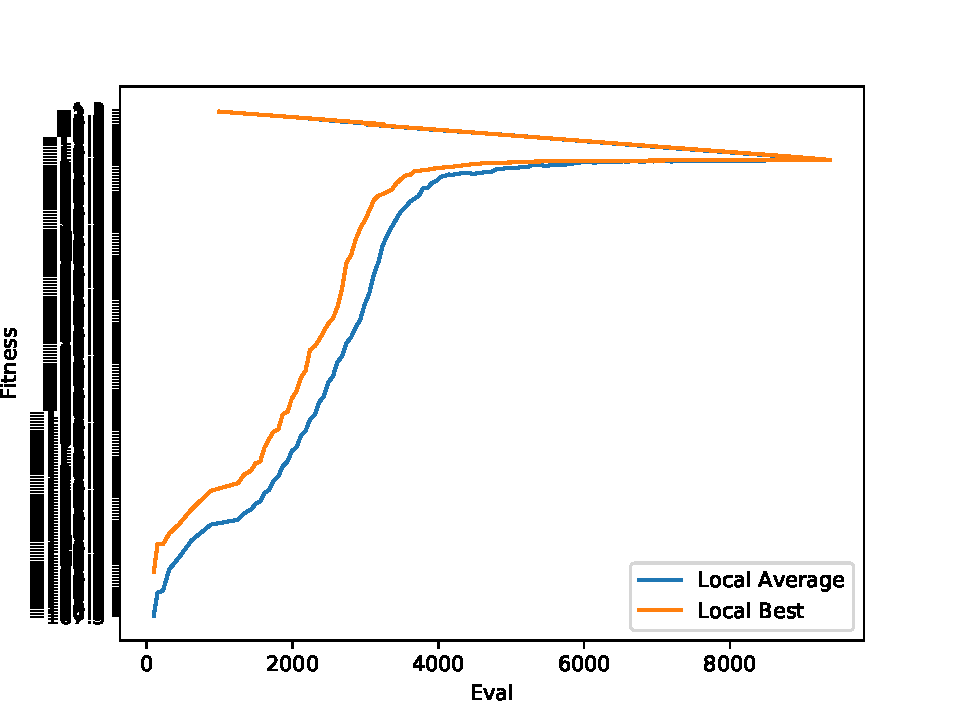
\includegraphics[width=\textwidth]{../graphs/graphs/1020.pdf}
\end{figure}


\clearpage
\begin{table}[!htb]
	\centering
	\caption{Figure \ref{fig:graph_1021} Configuration File}
	\label{tab:graph_1021}
	\begin{tabular}{| c | c |}
		\hline
		Self Adaptive Offspring Count		& False		 \\
		\hline
		Tournament Size For Parent Selection		& 5		 \\
		\hline
		Penalty Coefficient		& 1		 \\
		\hline
		Runs		& 30		 \\
		\hline
		Parent Selection Algorithm		& k-Tournament Selection with replacement		 \\
		\hline
		Self Adaptive Mutation Rate		& True		 \\
		\hline
		Offspring Count		& 50		 \\
		\hline
		Termination Convergence Criterion		& 10000		 \\
		\hline
		Solution File Path		& None		 \\
		\hline
		Mutation Rate		& 0.1		 \\
		\hline
		Recombination Algorithm		& Partially Mapped Crossover		 \\
		\hline
		Random Seed		& 1021		 \\
		\hline
		Mutation Algorithm		& Move		 \\
		\hline
		Tournament Size For Survival Selection		& 5		 \\
		\hline
		Placement Algorithm		& Random with Penalty		 \\
		\hline
		Population Size		& 100		 \\
		\hline
		Survival Strategy		& Plus		 \\
		\hline
		Search Algorithm		& EA		 \\
		\hline
		Log File Path		& None		 \\
		\hline
		Fitness Evaluations		& 10000		 \\
		\hline
		Survivor Algorithm		& Truncation		 \\
		\hline
		Self Adaptive Penalty Coefficient		& False		 \\
		\hline
	\end{tabular}
\end{table}
\begin{figure}[!htb]
	\caption{Input 1}
	\label{fig:graph_1021}
	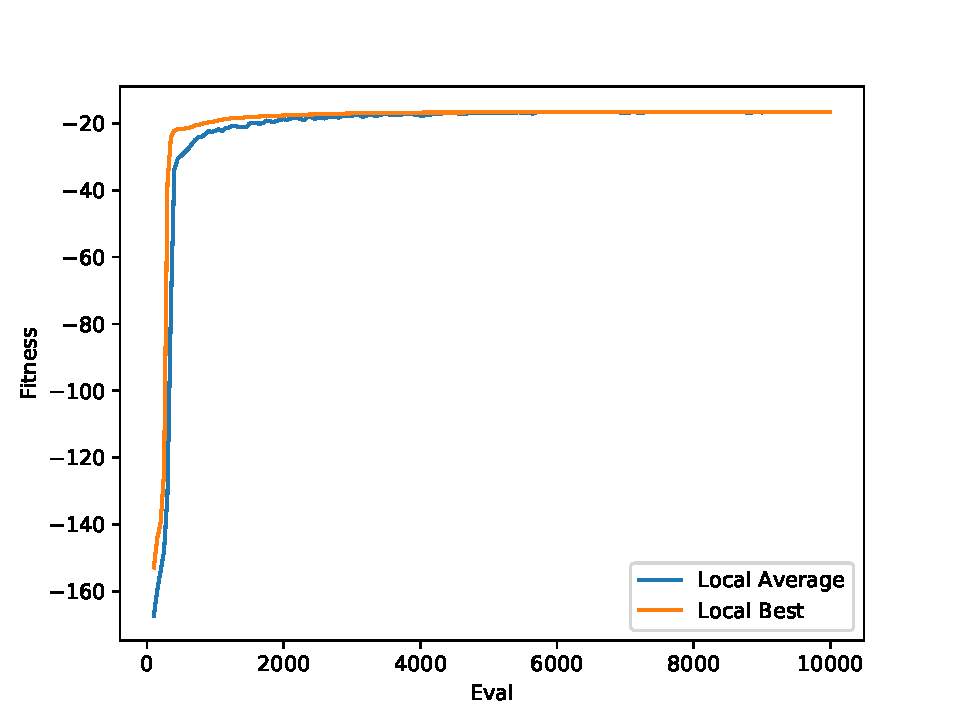
\includegraphics[width=\textwidth]{../graphs/graphs/1021.pdf}
\end{figure}


\begin{table}[!htb]
	\centering
	\caption{Figure \ref{fig:graph_1022} Configuration File}
	\label{tab:graph_1022}
	\begin{tabular}{| c | c |}
		\hline
		Self Adaptive Offspring Count		& True		 \\
		\hline
		Tournament Size For Parent Selection		& 5		 \\
		\hline
		Penalty Coefficient		& 1		 \\
		\hline
		Runs		& 30		 \\
		\hline
		Parent Selection Algorithm		& k-Tournament Selection with replacement		 \\
		\hline
		Self Adaptive Mutation Rate		& True		 \\
		\hline
		Offspring Count		& 50		 \\
		\hline
		Termination Convergence Criterion		& 10000		 \\
		\hline
		Solution File Path		& None		 \\
		\hline
		Mutation Rate		& 0.1		 \\
		\hline
		Recombination Algorithm		& Partially Mapped Crossover		 \\
		\hline
		Random Seed		& 1022		 \\
		\hline
		Mutation Algorithm		& Move		 \\
		\hline
		Tournament Size For Survival Selection		& 5		 \\
		\hline
		Placement Algorithm		& Random with Penalty		 \\
		\hline
		Population Size		& 100		 \\
		\hline
		Survival Strategy		& Plus		 \\
		\hline
		Search Algorithm		& EA		 \\
		\hline
		Log File Path		& None		 \\
		\hline
		Fitness Evaluations		& 10000		 \\
		\hline
		Survivor Algorithm		& Truncation		 \\
		\hline
		Self Adaptive Penalty Coefficient		& False		 \\
		\hline
	\end{tabular}
\end{table}
\begin{figure}[!htb]
	\caption{Input 1}
	\label{fig:graph_1022}
	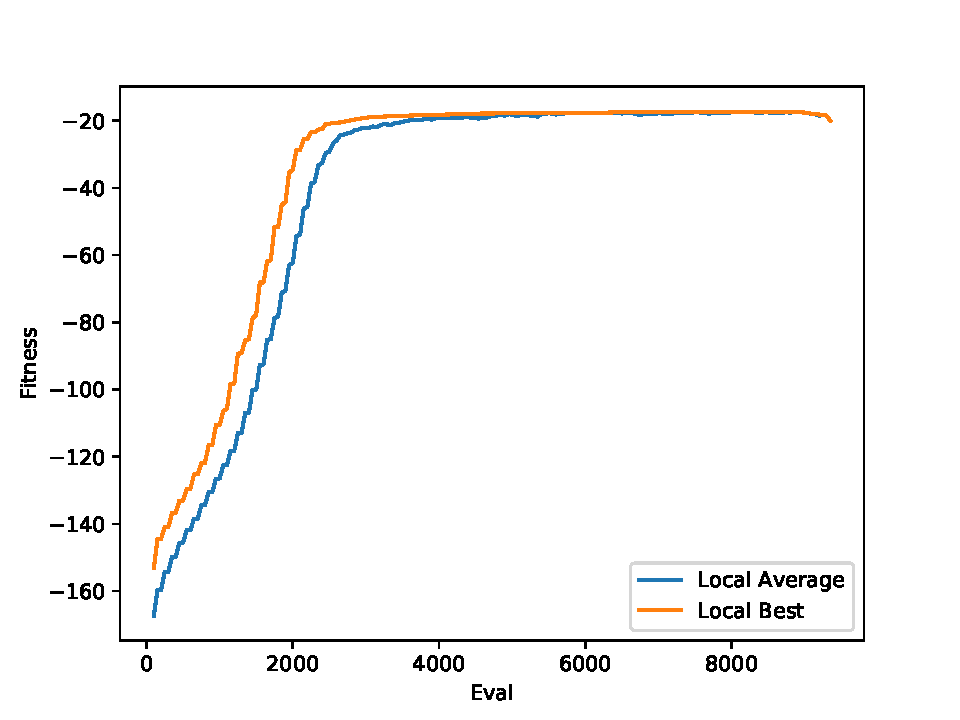
\includegraphics[width=\textwidth]{../graphs/graphs/1022.pdf}
\end{figure}


\begin{table}[!htb]
	\centering
	\caption{Figure \ref{fig:graph_1023} Configuration File}
	\label{tab:graph_1023}
	\begin{tabular}{| c | c |}
		\hline
		Self Adaptive Offspring Count		& False		 \\
		\hline
		Tournament Size For Parent Selection		& 5		 \\
		\hline
		Penalty Coefficient		& 1		 \\
		\hline
		Runs		& 30		 \\
		\hline
		Parent Selection Algorithm		& k-Tournament Selection with replacement		 \\
		\hline
		Self Adaptive Mutation Rate		& True		 \\
		\hline
		Offspring Count		& 50		 \\
		\hline
		Termination Convergence Criterion		& 10000		 \\
		\hline
		Solution File Path		& None		 \\
		\hline
		Mutation Rate		& 0.1		 \\
		\hline
		Recombination Algorithm		& Partially Mapped Crossover		 \\
		\hline
		Random Seed		& 1023		 \\
		\hline
		Mutation Algorithm		& Move		 \\
		\hline
		Tournament Size For Survival Selection		& 5		 \\
		\hline
		Placement Algorithm		& Random with Penalty		 \\
		\hline
		Population Size		& 100		 \\
		\hline
		Survival Strategy		& Plus		 \\
		\hline
		Search Algorithm		& EA		 \\
		\hline
		Log File Path		& None		 \\
		\hline
		Fitness Evaluations		& 10000		 \\
		\hline
		Survivor Algorithm		& Truncation		 \\
		\hline
		Self Adaptive Penalty Coefficient		& True		 \\
		\hline
	\end{tabular}
\end{table}
\begin{figure}[!htb]
	\caption{Input 1}
	\label{fig:graph_1023}
	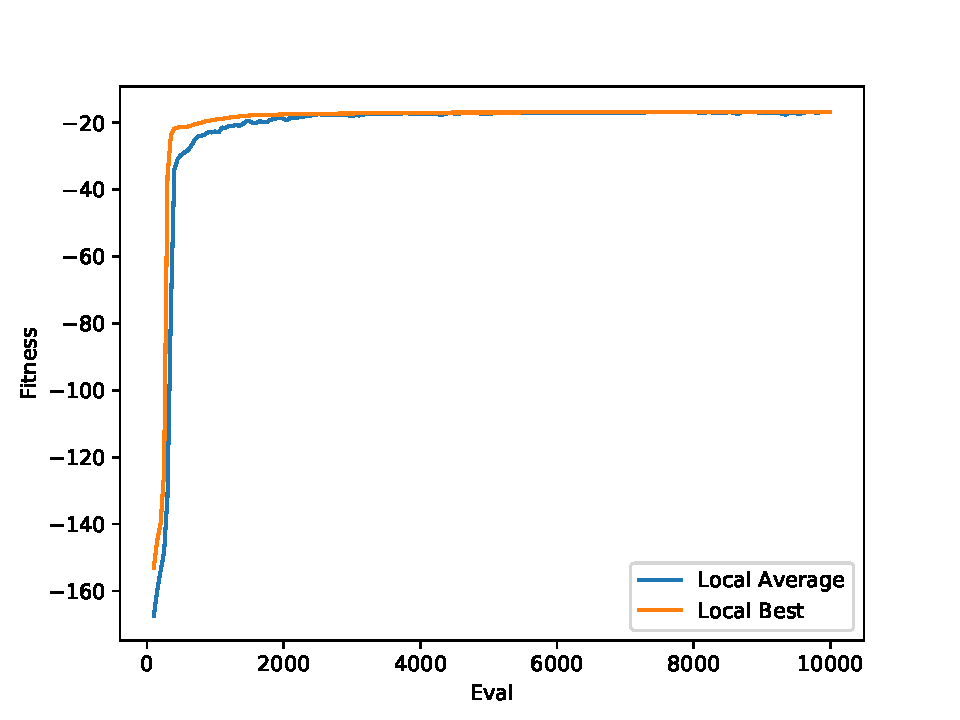
\includegraphics[width=\textwidth]{../graphs/graphs/1023.pdf}
\end{figure}


\begin{table}[!htb]
	\centering
	\caption{Figure \ref{fig:graph_1024} Configuration File}
	\label{tab:graph_1024}
	\begin{tabular}{| c | c |}
		\hline
		Self Adaptive Offspring Count		& True		 \\
		\hline
		Tournament Size For Parent Selection		& 5		 \\
		\hline
		Penalty Coefficient		& 1		 \\
		\hline
		Runs		& 30		 \\
		\hline
		Parent Selection Algorithm		& k-Tournament Selection with replacement		 \\
		\hline
		Self Adaptive Mutation Rate		& True		 \\
		\hline
		Offspring Count		& 50		 \\
		\hline
		Termination Convergence Criterion		& 10000		 \\
		\hline
		Solution File Path		& None		 \\
		\hline
		Mutation Rate		& 0.1		 \\
		\hline
		Recombination Algorithm		& Partially Mapped Crossover		 \\
		\hline
		Random Seed		& 1024		 \\
		\hline
		Mutation Algorithm		& Move		 \\
		\hline
		Tournament Size For Survival Selection		& 5		 \\
		\hline
		Placement Algorithm		& Random with Penalty		 \\
		\hline
		Population Size		& 100		 \\
		\hline
		Survival Strategy		& Plus		 \\
		\hline
		Search Algorithm		& EA		 \\
		\hline
		Log File Path		& None		 \\
		\hline
		Fitness Evaluations		& 10000		 \\
		\hline
		Survivor Algorithm		& Truncation		 \\
		\hline
		Self Adaptive Penalty Coefficient		& True		 \\
		\hline
	\end{tabular}
\end{table}
\begin{figure}[!htb]
	\caption{Input 1}
	\label{fig:graph_1024}
	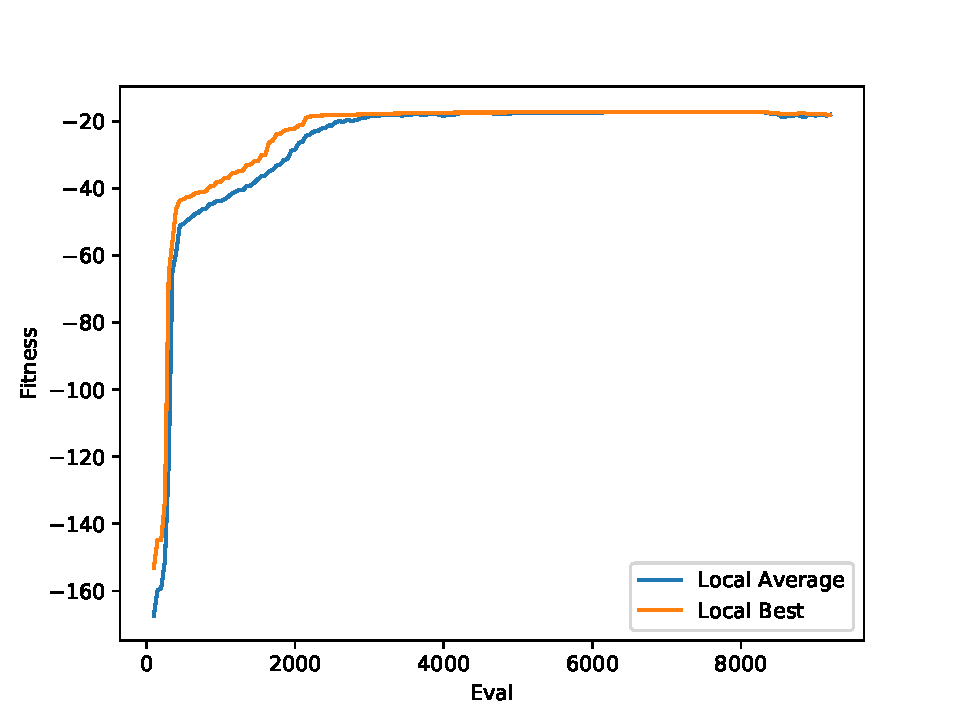
\includegraphics[width=\textwidth]{../graphs/graphs/1024.pdf}
\end{figure}


\begin{table}[!htb]
	\centering
	\caption{Figure \ref{fig:graph_1025} Configuration File}
	\label{tab:graph_1025}
	\begin{tabular}{| c | c |}
		\hline
		Self Adaptive Offspring Count		& False		 \\
		\hline
		Tournament Size For Parent Selection		& 5		 \\
		\hline
		Penalty Coefficient		& 1		 \\
		\hline
		Runs		& 30		 \\
		\hline
		Parent Selection Algorithm		& k-Tournament Selection with replacement		 \\
		\hline
		Self Adaptive Mutation Rate		& False		 \\
		\hline
		Offspring Count		& 50		 \\
		\hline
		Termination Convergence Criterion		& 10000		 \\
		\hline
		Solution File Path		& None		 \\
		\hline
		Mutation Rate		& 0.1		 \\
		\hline
		Recombination Algorithm		& Partially Mapped Crossover		 \\
		\hline
		Random Seed		& 1025		 \\
		\hline
		Mutation Algorithm		& Flip		 \\
		\hline
		Tournament Size For Survival Selection		& 5		 \\
		\hline
		Placement Algorithm		& Random		 \\
		\hline
		Population Size		& 100		 \\
		\hline
		Survival Strategy		& Plus		 \\
		\hline
		Search Algorithm		& EA		 \\
		\hline
		Log File Path		& None		 \\
		\hline
		Fitness Evaluations		& 10000		 \\
		\hline
		Survivor Algorithm		& Truncation		 \\
		\hline
		Self Adaptive Penalty Coefficient		& False		 \\
		\hline
	\end{tabular}
\end{table}
\begin{figure}[!htb]
	\caption{Input 1}
	\label{fig:graph_1025}
	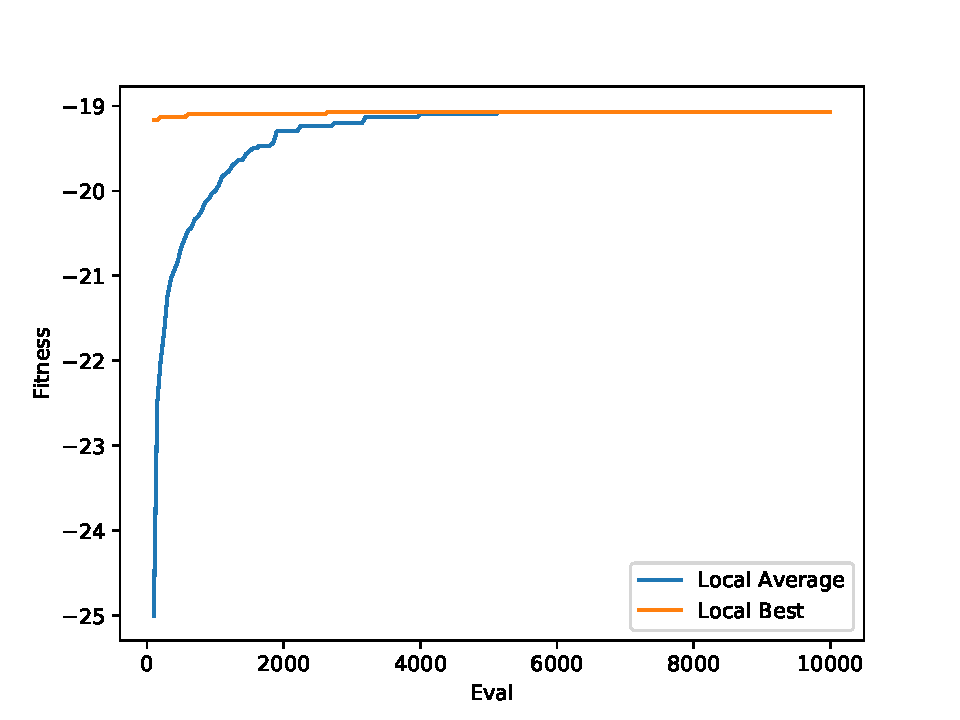
\includegraphics[width=\textwidth]{../graphs/graphs/1025.pdf}
\end{figure}


\begin{table}[!htb]
	\centering
	\caption{Figure \ref{fig:graph_1026} Configuration File}
	\label{tab:graph_1026}
	\begin{tabular}{| c | c |}
		\hline
		Self Adaptive Offspring Count		& True		 \\
		\hline
		Tournament Size For Parent Selection		& 5		 \\
		\hline
		Penalty Coefficient		& 1		 \\
		\hline
		Runs		& 30		 \\
		\hline
		Parent Selection Algorithm		& k-Tournament Selection with replacement		 \\
		\hline
		Self Adaptive Mutation Rate		& False		 \\
		\hline
		Offspring Count		& 50		 \\
		\hline
		Termination Convergence Criterion		& 10000		 \\
		\hline
		Solution File Path		& None		 \\
		\hline
		Mutation Rate		& 0.1		 \\
		\hline
		Recombination Algorithm		& Partially Mapped Crossover		 \\
		\hline
		Random Seed		& 1026		 \\
		\hline
		Mutation Algorithm		& Flip		 \\
		\hline
		Tournament Size For Survival Selection		& 5		 \\
		\hline
		Placement Algorithm		& Random		 \\
		\hline
		Population Size		& 100		 \\
		\hline
		Survival Strategy		& Plus		 \\
		\hline
		Search Algorithm		& EA		 \\
		\hline
		Log File Path		& None		 \\
		\hline
		Fitness Evaluations		& 10000		 \\
		\hline
		Survivor Algorithm		& Truncation		 \\
		\hline
		Self Adaptive Penalty Coefficient		& False		 \\
		\hline
	\end{tabular}
\end{table}
\begin{figure}[!htb]
	\caption{Input 1}
	\label{fig:graph_1026}
	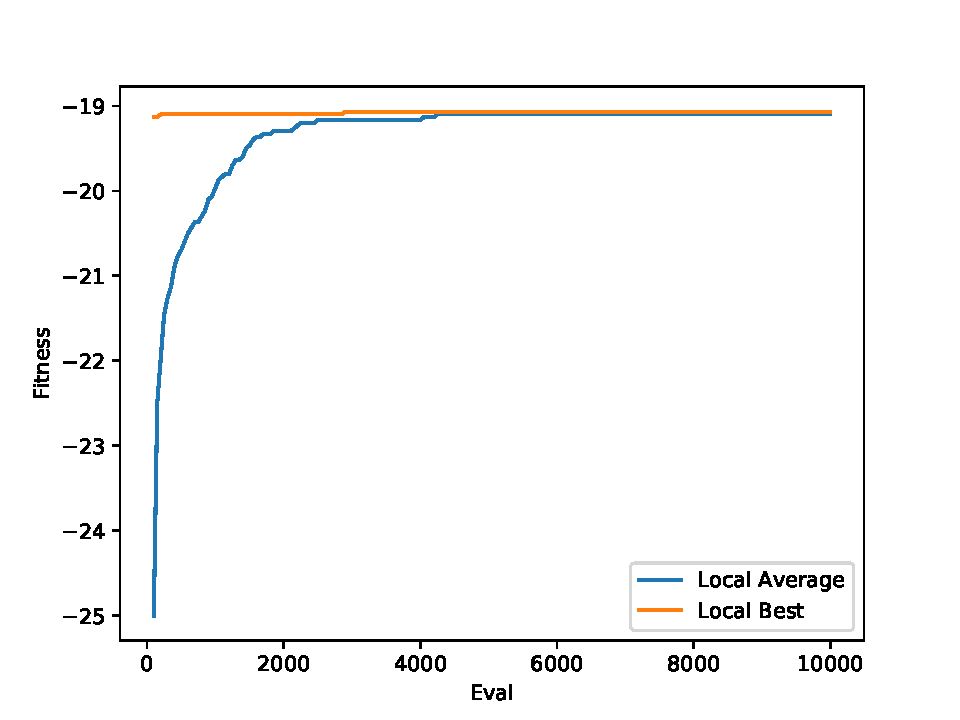
\includegraphics[width=\textwidth]{../graphs/graphs/1026.pdf}
\end{figure}


\begin{table}[!htb]
	\centering
	\caption{Figure \ref{fig:graph_1027} Configuration File}
	\label{tab:graph_1027}
	\begin{tabular}{| c | c |}
		\hline
		Self Adaptive Offspring Count		& False		 \\
		\hline
		Tournament Size For Parent Selection		& 5		 \\
		\hline
		Penalty Coefficient		& 1		 \\
		\hline
		Runs		& 30		 \\
		\hline
		Parent Selection Algorithm		& k-Tournament Selection with replacement		 \\
		\hline
		Self Adaptive Mutation Rate		& False		 \\
		\hline
		Offspring Count		& 50		 \\
		\hline
		Termination Convergence Criterion		& 10000		 \\
		\hline
		Solution File Path		& None		 \\
		\hline
		Mutation Rate		& 0.1		 \\
		\hline
		Recombination Algorithm		& Partially Mapped Crossover		 \\
		\hline
		Random Seed		& 1027		 \\
		\hline
		Mutation Algorithm		& Flip		 \\
		\hline
		Tournament Size For Survival Selection		& 5		 \\
		\hline
		Placement Algorithm		& Random		 \\
		\hline
		Population Size		& 100		 \\
		\hline
		Survival Strategy		& Plus		 \\
		\hline
		Search Algorithm		& EA		 \\
		\hline
		Log File Path		& None		 \\
		\hline
		Fitness Evaluations		& 10000		 \\
		\hline
		Survivor Algorithm		& Truncation		 \\
		\hline
		Self Adaptive Penalty Coefficient		& True		 \\
		\hline
	\end{tabular}
\end{table}
\begin{figure}[!htb]
	\caption{Input 1}
	\label{fig:graph_1027}
	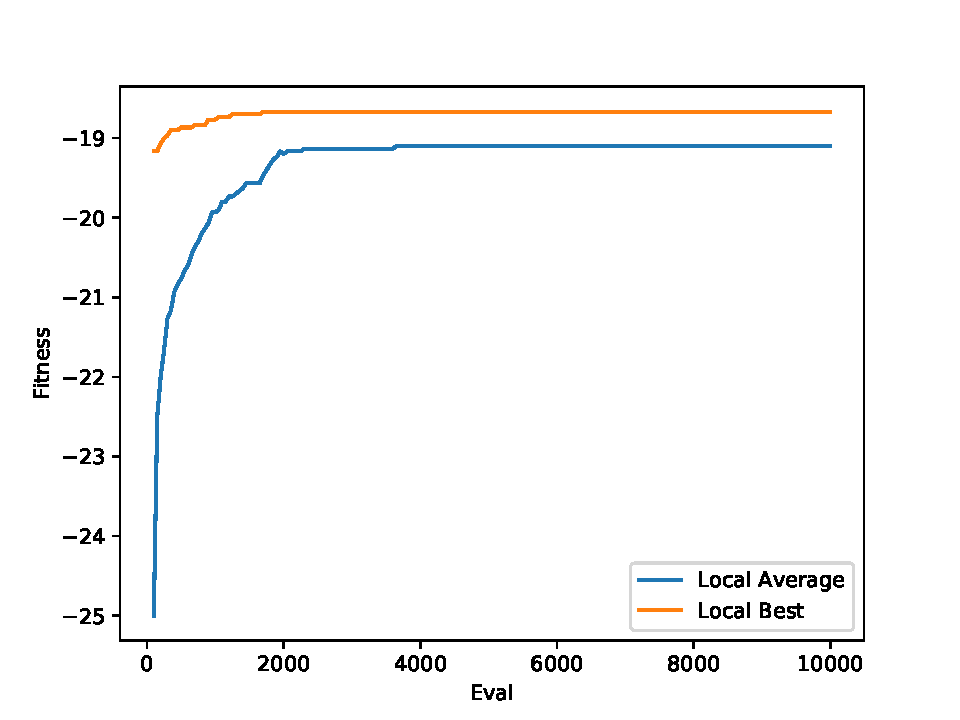
\includegraphics[width=\textwidth]{../graphs/graphs/1027.pdf}
\end{figure}


\begin{table}[!htb]
	\centering
	\caption{Figure \ref{fig:graph_1028} Configuration File}
	\label{tab:graph_1028}
	\begin{tabular}{| c | c |}
		\hline
		Self Adaptive Offspring Count		& True		 \\
		\hline
		Tournament Size For Parent Selection		& 5		 \\
		\hline
		Penalty Coefficient		& 1		 \\
		\hline
		Runs		& 30		 \\
		\hline
		Parent Selection Algorithm		& k-Tournament Selection with replacement		 \\
		\hline
		Self Adaptive Mutation Rate		& False		 \\
		\hline
		Offspring Count		& 50		 \\
		\hline
		Termination Convergence Criterion		& 10000		 \\
		\hline
		Solution File Path		& None		 \\
		\hline
		Mutation Rate		& 0.1		 \\
		\hline
		Recombination Algorithm		& Partially Mapped Crossover		 \\
		\hline
		Random Seed		& 1028		 \\
		\hline
		Mutation Algorithm		& Flip		 \\
		\hline
		Tournament Size For Survival Selection		& 5		 \\
		\hline
		Placement Algorithm		& Random		 \\
		\hline
		Population Size		& 100		 \\
		\hline
		Survival Strategy		& Plus		 \\
		\hline
		Search Algorithm		& EA		 \\
		\hline
		Log File Path		& None		 \\
		\hline
		Fitness Evaluations		& 10000		 \\
		\hline
		Survivor Algorithm		& Truncation		 \\
		\hline
		Self Adaptive Penalty Coefficient		& True		 \\
		\hline
	\end{tabular}
\end{table}
\begin{figure}[!htb]
	\caption{Input 1}
	\label{fig:graph_1028}
	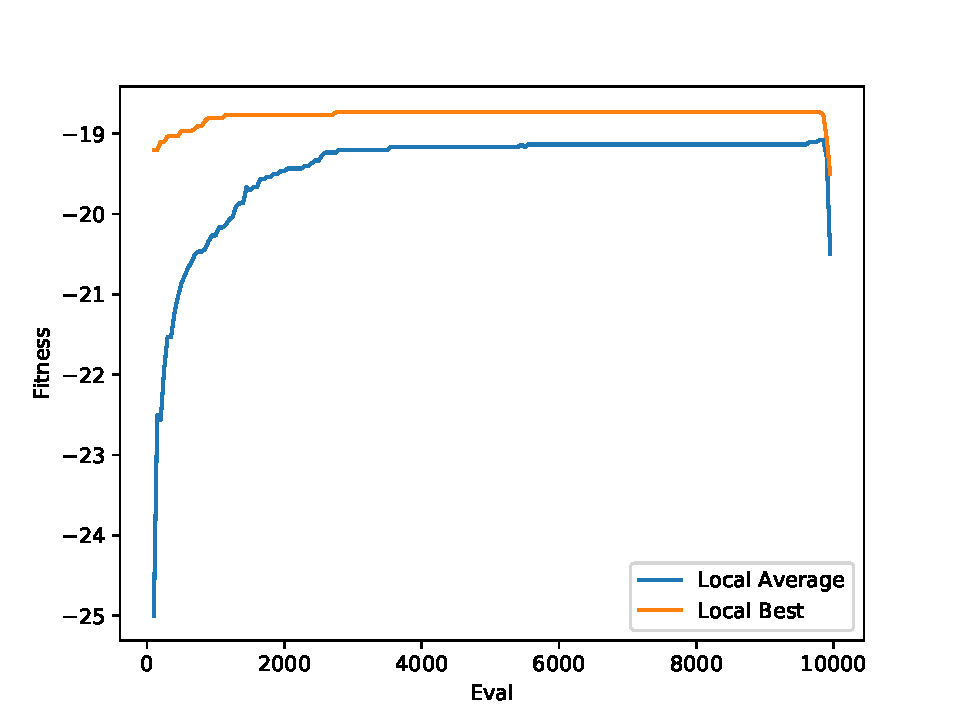
\includegraphics[width=\textwidth]{../graphs/graphs/1028.pdf}
\end{figure}


\begin{table}[!htb]
	\centering
	\caption{Figure \ref{fig:graph_1029} Configuration File}
	\label{tab:graph_1029}
	\begin{tabular}{| c | c |}
		\hline
		Self Adaptive Offspring Count		& False		 \\
		\hline
		Tournament Size For Parent Selection		& 5		 \\
		\hline
		Penalty Coefficient		& 1		 \\
		\hline
		Runs		& 30		 \\
		\hline
		Parent Selection Algorithm		& k-Tournament Selection with replacement		 \\
		\hline
		Self Adaptive Mutation Rate		& True		 \\
		\hline
		Offspring Count		& 50		 \\
		\hline
		Termination Convergence Criterion		& 10000		 \\
		\hline
		Solution File Path		& None		 \\
		\hline
		Mutation Rate		& 0.1		 \\
		\hline
		Recombination Algorithm		& Partially Mapped Crossover		 \\
		\hline
		Random Seed		& 1029		 \\
		\hline
		Mutation Algorithm		& Flip		 \\
		\hline
		Tournament Size For Survival Selection		& 5		 \\
		\hline
		Placement Algorithm		& Random		 \\
		\hline
		Population Size		& 100		 \\
		\hline
		Survival Strategy		& Plus		 \\
		\hline
		Search Algorithm		& EA		 \\
		\hline
		Log File Path		& None		 \\
		\hline
		Fitness Evaluations		& 10000		 \\
		\hline
		Survivor Algorithm		& Truncation		 \\
		\hline
		Self Adaptive Penalty Coefficient		& False		 \\
		\hline
	\end{tabular}
\end{table}
\begin{figure}[!htb]
	\caption{Input 1}
	\label{fig:graph_1029}
	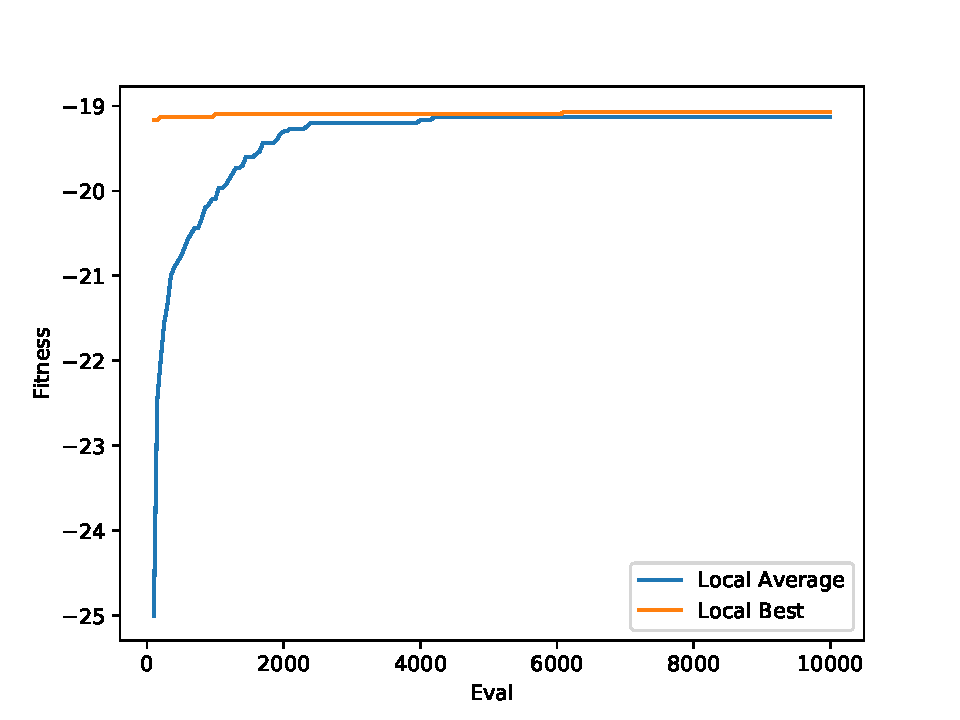
\includegraphics[width=\textwidth]{../graphs/graphs/1029.pdf}
\end{figure}


\begin{table}[!htb]
	\centering
	\caption{Figure \ref{fig:graph_1030} Configuration File}
	\label{tab:graph_1030}
	\begin{tabular}{| c | c |}
		\hline
		Self Adaptive Offspring Count		& True		 \\
		\hline
		Tournament Size For Parent Selection		& 5		 \\
		\hline
		Penalty Coefficient		& 1		 \\
		\hline
		Runs		& 30		 \\
		\hline
		Parent Selection Algorithm		& k-Tournament Selection with replacement		 \\
		\hline
		Self Adaptive Mutation Rate		& True		 \\
		\hline
		Offspring Count		& 50		 \\
		\hline
		Termination Convergence Criterion		& 10000		 \\
		\hline
		Solution File Path		& None		 \\
		\hline
		Mutation Rate		& 0.1		 \\
		\hline
		Recombination Algorithm		& Partially Mapped Crossover		 \\
		\hline
		Random Seed		& 1030		 \\
		\hline
		Mutation Algorithm		& Flip		 \\
		\hline
		Tournament Size For Survival Selection		& 5		 \\
		\hline
		Placement Algorithm		& Random		 \\
		\hline
		Population Size		& 100		 \\
		\hline
		Survival Strategy		& Plus		 \\
		\hline
		Search Algorithm		& EA		 \\
		\hline
		Log File Path		& None		 \\
		\hline
		Fitness Evaluations		& 10000		 \\
		\hline
		Survivor Algorithm		& Truncation		 \\
		\hline
		Self Adaptive Penalty Coefficient		& False		 \\
		\hline
	\end{tabular}
\end{table}
\begin{figure}[!htb]
	\caption{Input 1}
	\label{fig:graph_1030}
	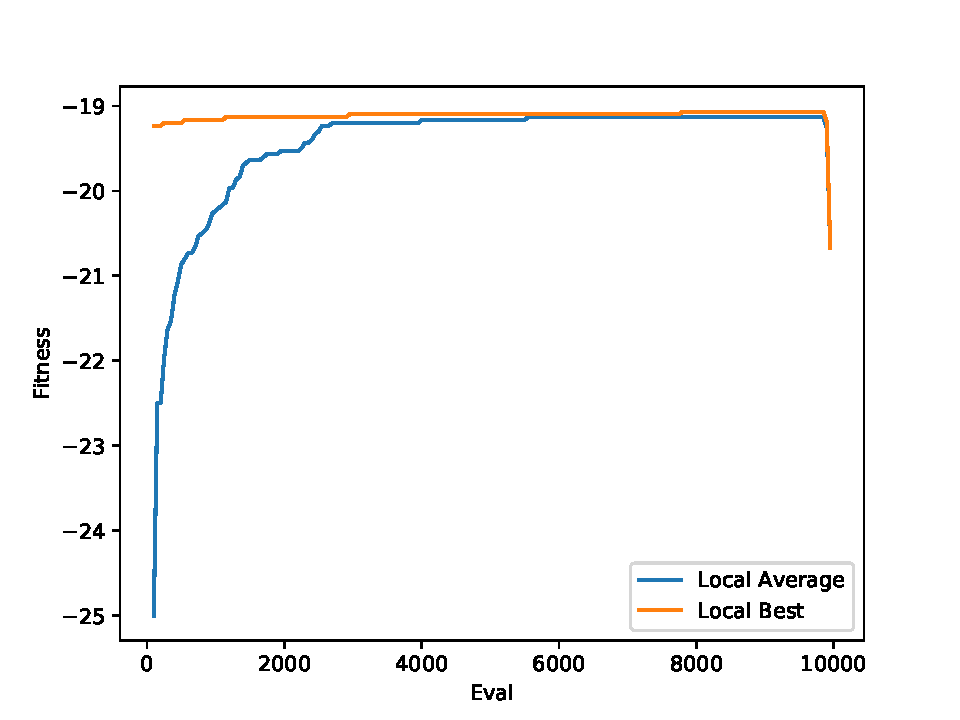
\includegraphics[width=\textwidth]{../graphs/graphs/1030.pdf}
\end{figure}


\clearpage
\begin{table}[!htb]
	\centering
	\caption{Figure \ref{fig:graph_1031} Configuration File}
	\label{tab:graph_1031}
	\begin{tabular}{| c | c |}
		\hline
		Self Adaptive Offspring Count		& False		 \\
		\hline
		Tournament Size For Parent Selection		& 5		 \\
		\hline
		Penalty Coefficient		& 1		 \\
		\hline
		Runs		& 30		 \\
		\hline
		Parent Selection Algorithm		& k-Tournament Selection with replacement		 \\
		\hline
		Self Adaptive Mutation Rate		& True		 \\
		\hline
		Offspring Count		& 50		 \\
		\hline
		Termination Convergence Criterion		& 10000		 \\
		\hline
		Solution File Path		& None		 \\
		\hline
		Mutation Rate		& 0.1		 \\
		\hline
		Recombination Algorithm		& Partially Mapped Crossover		 \\
		\hline
		Random Seed		& 1031		 \\
		\hline
		Mutation Algorithm		& Flip		 \\
		\hline
		Tournament Size For Survival Selection		& 5		 \\
		\hline
		Placement Algorithm		& Random		 \\
		\hline
		Population Size		& 100		 \\
		\hline
		Survival Strategy		& Plus		 \\
		\hline
		Search Algorithm		& EA		 \\
		\hline
		Log File Path		& None		 \\
		\hline
		Fitness Evaluations		& 10000		 \\
		\hline
		Survivor Algorithm		& Truncation		 \\
		\hline
		Self Adaptive Penalty Coefficient		& True		 \\
		\hline
	\end{tabular}
\end{table}
\begin{figure}[!htb]
	\caption{Input 1}
	\label{fig:graph_1031}
	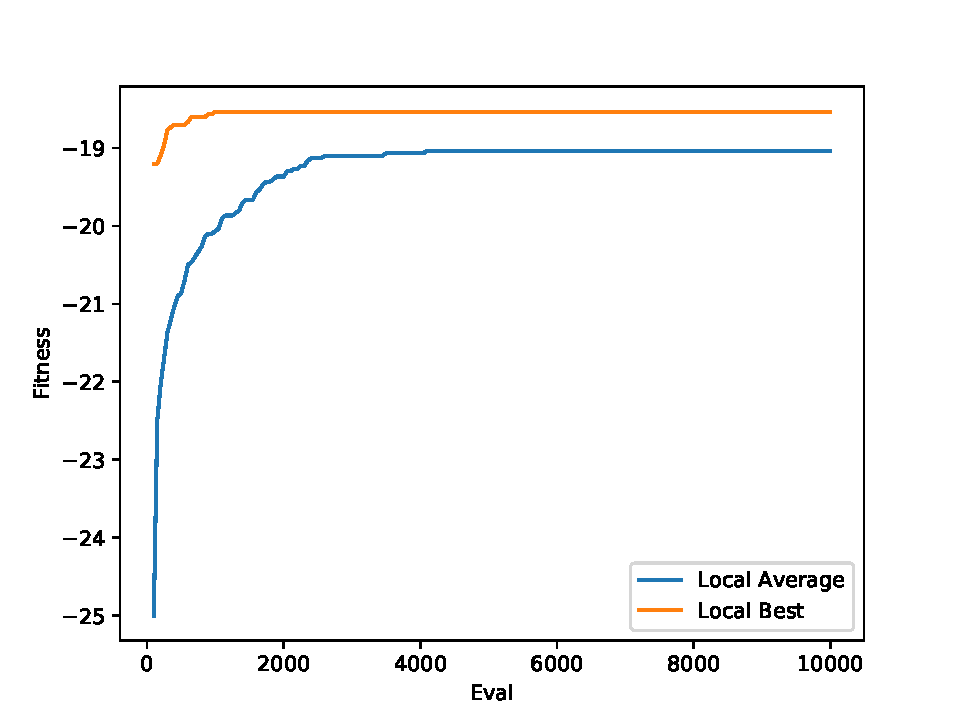
\includegraphics[width=\textwidth]{../graphs/graphs/1031.pdf}
\end{figure}


\begin{table}[!htb]
	\centering
	\caption{Figure \ref{fig:graph_1032} Configuration File}
	\label{tab:graph_1032}
	\begin{tabular}{| c | c |}
		\hline
		Self Adaptive Offspring Count		& True		 \\
		\hline
		Tournament Size For Parent Selection		& 5		 \\
		\hline
		Penalty Coefficient		& 1		 \\
		\hline
		Runs		& 30		 \\
		\hline
		Parent Selection Algorithm		& k-Tournament Selection with replacement		 \\
		\hline
		Self Adaptive Mutation Rate		& True		 \\
		\hline
		Offspring Count		& 50		 \\
		\hline
		Termination Convergence Criterion		& 10000		 \\
		\hline
		Solution File Path		& None		 \\
		\hline
		Mutation Rate		& 0.1		 \\
		\hline
		Recombination Algorithm		& Partially Mapped Crossover		 \\
		\hline
		Random Seed		& 1032		 \\
		\hline
		Mutation Algorithm		& Flip		 \\
		\hline
		Tournament Size For Survival Selection		& 5		 \\
		\hline
		Placement Algorithm		& Random		 \\
		\hline
		Population Size		& 100		 \\
		\hline
		Survival Strategy		& Plus		 \\
		\hline
		Search Algorithm		& EA		 \\
		\hline
		Log File Path		& None		 \\
		\hline
		Fitness Evaluations		& 10000		 \\
		\hline
		Survivor Algorithm		& Truncation		 \\
		\hline
		Self Adaptive Penalty Coefficient		& True		 \\
		\hline
	\end{tabular}
\end{table}
\begin{figure}[!htb]
	\caption{Input 1}
	\label{fig:graph_1032}
	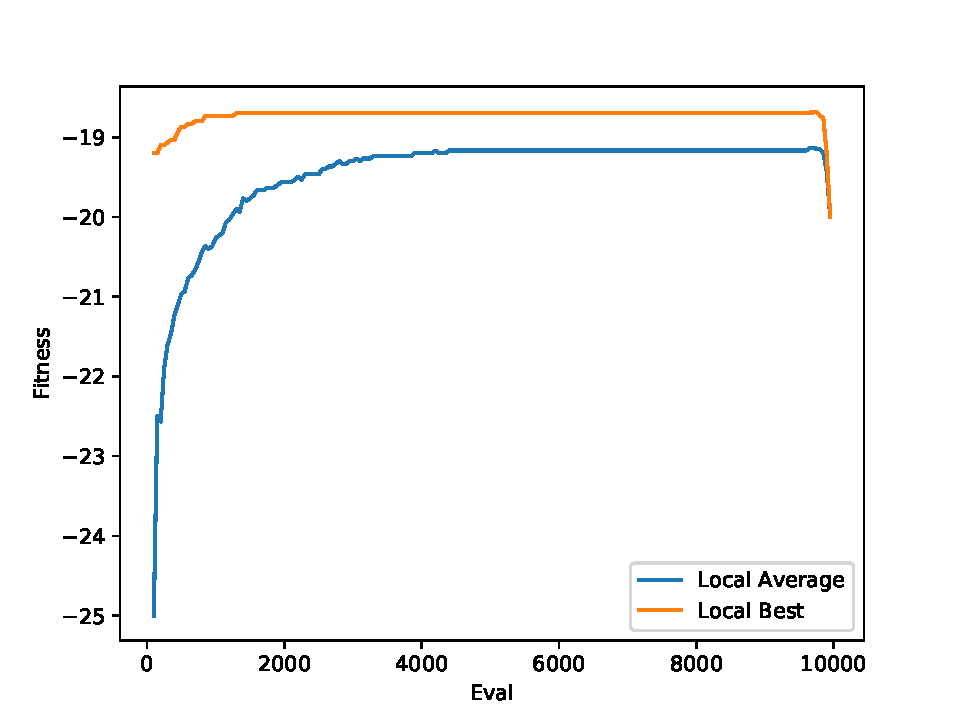
\includegraphics[width=\textwidth]{../graphs/graphs/1032.pdf}
\end{figure}


\begin{table}[!htb]
	\centering
	\caption{Figure \ref{fig:graph_1033} Configuration File}
	\label{tab:graph_1033}
	\begin{tabular}{| c | c |}
		\hline
		Self Adaptive Offspring Count		& False		 \\
		\hline
		Tournament Size For Parent Selection		& 5		 \\
		\hline
		Penalty Coefficient		& 1		 \\
		\hline
		Runs		& 30		 \\
		\hline
		Parent Selection Algorithm		& k-Tournament Selection with replacement		 \\
		\hline
		Self Adaptive Mutation Rate		& False		 \\
		\hline
		Offspring Count		& 50		 \\
		\hline
		Termination Convergence Criterion		& 10000		 \\
		\hline
		Solution File Path		& None		 \\
		\hline
		Mutation Rate		& 0.1		 \\
		\hline
		Recombination Algorithm		& Partially Mapped Crossover		 \\
		\hline
		Random Seed		& 1033		 \\
		\hline
		Mutation Algorithm		& Flip		 \\
		\hline
		Tournament Size For Survival Selection		& 5		 \\
		\hline
		Placement Algorithm		& Random with Repair		 \\
		\hline
		Population Size		& 100		 \\
		\hline
		Survival Strategy		& Plus		 \\
		\hline
		Search Algorithm		& EA		 \\
		\hline
		Log File Path		& None		 \\
		\hline
		Fitness Evaluations		& 10000		 \\
		\hline
		Survivor Algorithm		& Truncation		 \\
		\hline
		Self Adaptive Penalty Coefficient		& False		 \\
		\hline
	\end{tabular}
\end{table}
\begin{figure}[!htb]
	\caption{Input 1}
	\label{fig:graph_1033}
	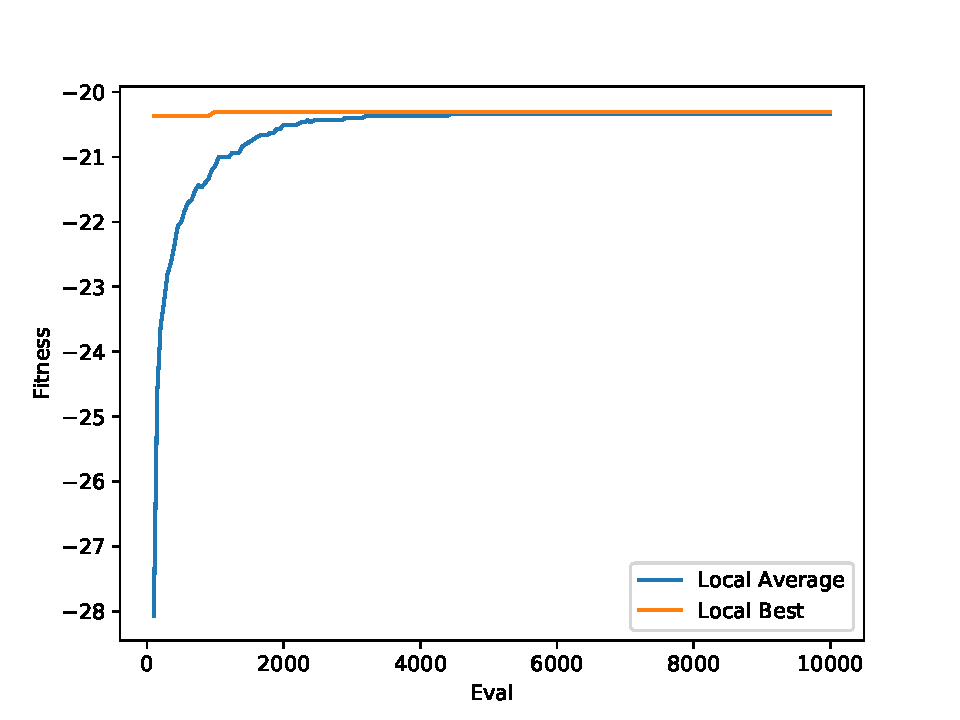
\includegraphics[width=\textwidth]{../graphs/graphs/1033.pdf}
\end{figure}


\begin{table}[!htb]
	\centering
	\caption{Figure \ref{fig:graph_1034} Configuration File}
	\label{tab:graph_1034}
	\begin{tabular}{| c | c |}
		\hline
		Self Adaptive Offspring Count		& True		 \\
		\hline
		Tournament Size For Parent Selection		& 5		 \\
		\hline
		Penalty Coefficient		& 1		 \\
		\hline
		Runs		& 30		 \\
		\hline
		Parent Selection Algorithm		& k-Tournament Selection with replacement		 \\
		\hline
		Self Adaptive Mutation Rate		& False		 \\
		\hline
		Offspring Count		& 50		 \\
		\hline
		Termination Convergence Criterion		& 10000		 \\
		\hline
		Solution File Path		& None		 \\
		\hline
		Mutation Rate		& 0.1		 \\
		\hline
		Recombination Algorithm		& Partially Mapped Crossover		 \\
		\hline
		Random Seed		& 1034		 \\
		\hline
		Mutation Algorithm		& Flip		 \\
		\hline
		Tournament Size For Survival Selection		& 5		 \\
		\hline
		Placement Algorithm		& Random with Repair		 \\
		\hline
		Population Size		& 100		 \\
		\hline
		Survival Strategy		& Plus		 \\
		\hline
		Search Algorithm		& EA		 \\
		\hline
		Log File Path		& None		 \\
		\hline
		Fitness Evaluations		& 10000		 \\
		\hline
		Survivor Algorithm		& Truncation		 \\
		\hline
		Self Adaptive Penalty Coefficient		& False		 \\
		\hline
	\end{tabular}
\end{table}
\begin{figure}[!htb]
	\caption{Input 1}
	\label{fig:graph_1034}
	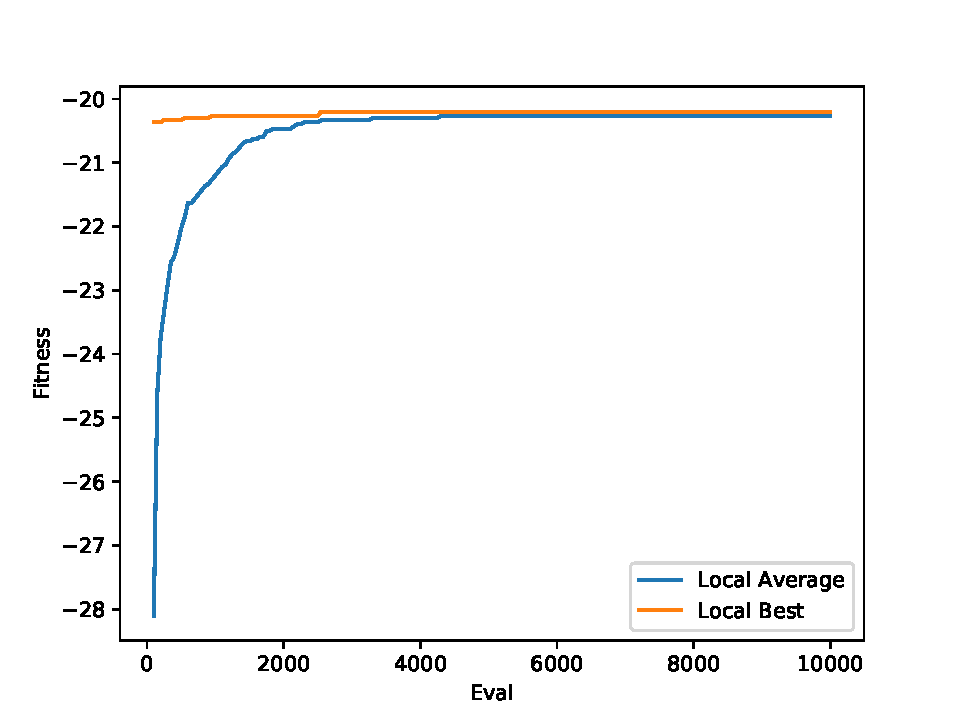
\includegraphics[width=\textwidth]{../graphs/graphs/1034.pdf}
\end{figure}


\begin{table}[!htb]
	\centering
	\caption{Figure \ref{fig:graph_1035} Configuration File}
	\label{tab:graph_1035}
	\begin{tabular}{| c | c |}
		\hline
		Self Adaptive Offspring Count		& False		 \\
		\hline
		Tournament Size For Parent Selection		& 5		 \\
		\hline
		Penalty Coefficient		& 1		 \\
		\hline
		Runs		& 30		 \\
		\hline
		Parent Selection Algorithm		& k-Tournament Selection with replacement		 \\
		\hline
		Self Adaptive Mutation Rate		& False		 \\
		\hline
		Offspring Count		& 50		 \\
		\hline
		Termination Convergence Criterion		& 10000		 \\
		\hline
		Solution File Path		& None		 \\
		\hline
		Mutation Rate		& 0.1		 \\
		\hline
		Recombination Algorithm		& Partially Mapped Crossover		 \\
		\hline
		Random Seed		& 1035		 \\
		\hline
		Mutation Algorithm		& Flip		 \\
		\hline
		Tournament Size For Survival Selection		& 5		 \\
		\hline
		Placement Algorithm		& Random with Repair		 \\
		\hline
		Population Size		& 100		 \\
		\hline
		Survival Strategy		& Plus		 \\
		\hline
		Search Algorithm		& EA		 \\
		\hline
		Log File Path		& None		 \\
		\hline
		Fitness Evaluations		& 10000		 \\
		\hline
		Survivor Algorithm		& Truncation		 \\
		\hline
		Self Adaptive Penalty Coefficient		& True		 \\
		\hline
	\end{tabular}
\end{table}
\begin{figure}[!htb]
	\caption{Input 1}
	\label{fig:graph_1035}
	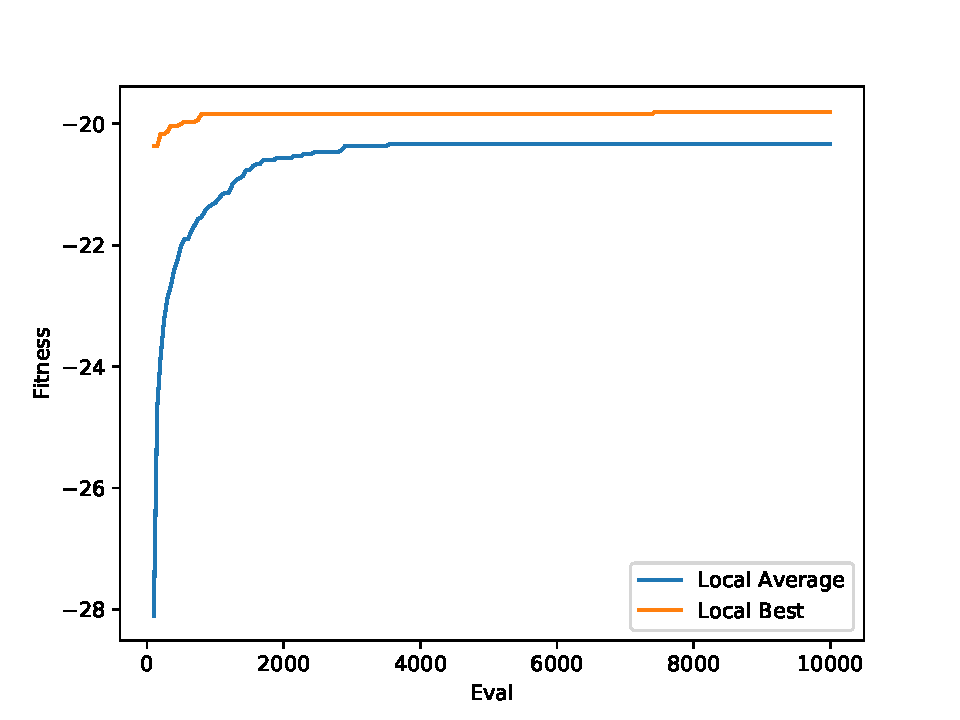
\includegraphics[width=\textwidth]{../graphs/graphs/1035.pdf}
\end{figure}


\begin{table}[!htb]
	\centering
	\caption{Figure \ref{fig:graph_1036} Configuration File}
	\label{tab:graph_1036}
	\begin{tabular}{| c | c |}
		\hline
		Self Adaptive Offspring Count		& True		 \\
		\hline
		Tournament Size For Parent Selection		& 5		 \\
		\hline
		Penalty Coefficient		& 1		 \\
		\hline
		Runs		& 30		 \\
		\hline
		Parent Selection Algorithm		& k-Tournament Selection with replacement		 \\
		\hline
		Self Adaptive Mutation Rate		& False		 \\
		\hline
		Offspring Count		& 50		 \\
		\hline
		Termination Convergence Criterion		& 10000		 \\
		\hline
		Solution File Path		& None		 \\
		\hline
		Mutation Rate		& 0.1		 \\
		\hline
		Recombination Algorithm		& Partially Mapped Crossover		 \\
		\hline
		Random Seed		& 1036		 \\
		\hline
		Mutation Algorithm		& Flip		 \\
		\hline
		Tournament Size For Survival Selection		& 5		 \\
		\hline
		Placement Algorithm		& Random with Repair		 \\
		\hline
		Population Size		& 100		 \\
		\hline
		Survival Strategy		& Plus		 \\
		\hline
		Search Algorithm		& EA		 \\
		\hline
		Log File Path		& None		 \\
		\hline
		Fitness Evaluations		& 10000		 \\
		\hline
		Survivor Algorithm		& Truncation		 \\
		\hline
		Self Adaptive Penalty Coefficient		& True		 \\
		\hline
	\end{tabular}
\end{table}
\begin{figure}[!htb]
	\caption{Input 1}
	\label{fig:graph_1036}
	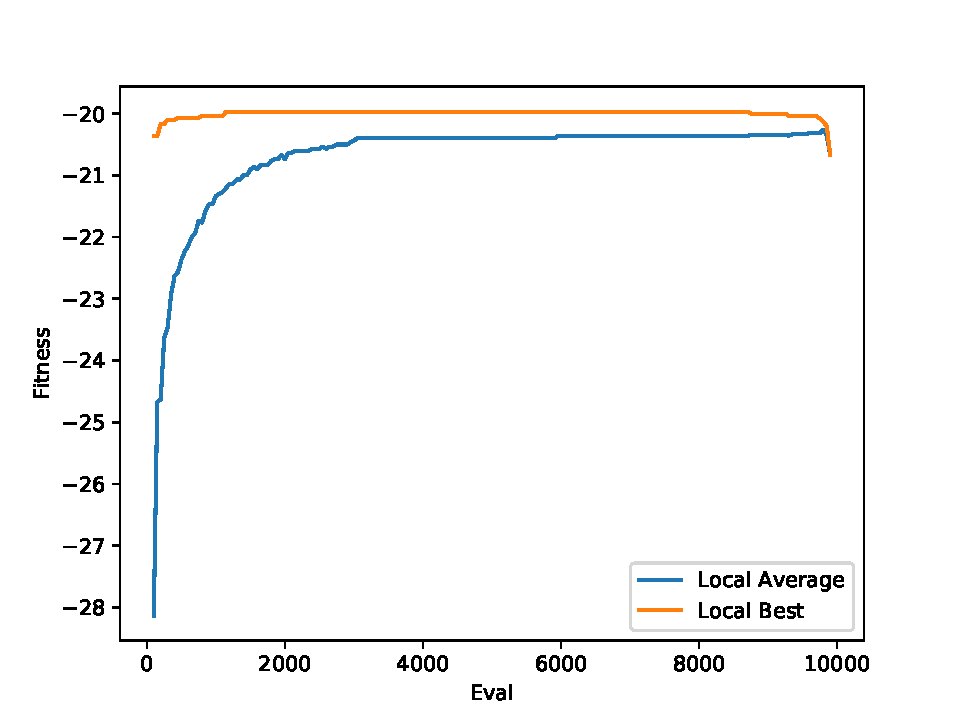
\includegraphics[width=\textwidth]{../graphs/graphs/1036.pdf}
\end{figure}


\begin{table}[!htb]
	\centering
	\caption{Figure \ref{fig:graph_1037} Configuration File}
	\label{tab:graph_1037}
	\begin{tabular}{| c | c |}
		\hline
		Self Adaptive Offspring Count		& False		 \\
		\hline
		Tournament Size For Parent Selection		& 5		 \\
		\hline
		Penalty Coefficient		& 1		 \\
		\hline
		Runs		& 30		 \\
		\hline
		Parent Selection Algorithm		& k-Tournament Selection with replacement		 \\
		\hline
		Self Adaptive Mutation Rate		& True		 \\
		\hline
		Offspring Count		& 50		 \\
		\hline
		Termination Convergence Criterion		& 10000		 \\
		\hline
		Solution File Path		& None		 \\
		\hline
		Mutation Rate		& 0.1		 \\
		\hline
		Recombination Algorithm		& Partially Mapped Crossover		 \\
		\hline
		Random Seed		& 1037		 \\
		\hline
		Mutation Algorithm		& Flip		 \\
		\hline
		Tournament Size For Survival Selection		& 5		 \\
		\hline
		Placement Algorithm		& Random with Repair		 \\
		\hline
		Population Size		& 100		 \\
		\hline
		Survival Strategy		& Plus		 \\
		\hline
		Search Algorithm		& EA		 \\
		\hline
		Log File Path		& None		 \\
		\hline
		Fitness Evaluations		& 10000		 \\
		\hline
		Survivor Algorithm		& Truncation		 \\
		\hline
		Self Adaptive Penalty Coefficient		& False		 \\
		\hline
	\end{tabular}
\end{table}
\begin{figure}[!htb]
	\caption{Input 1}
	\label{fig:graph_1037}
	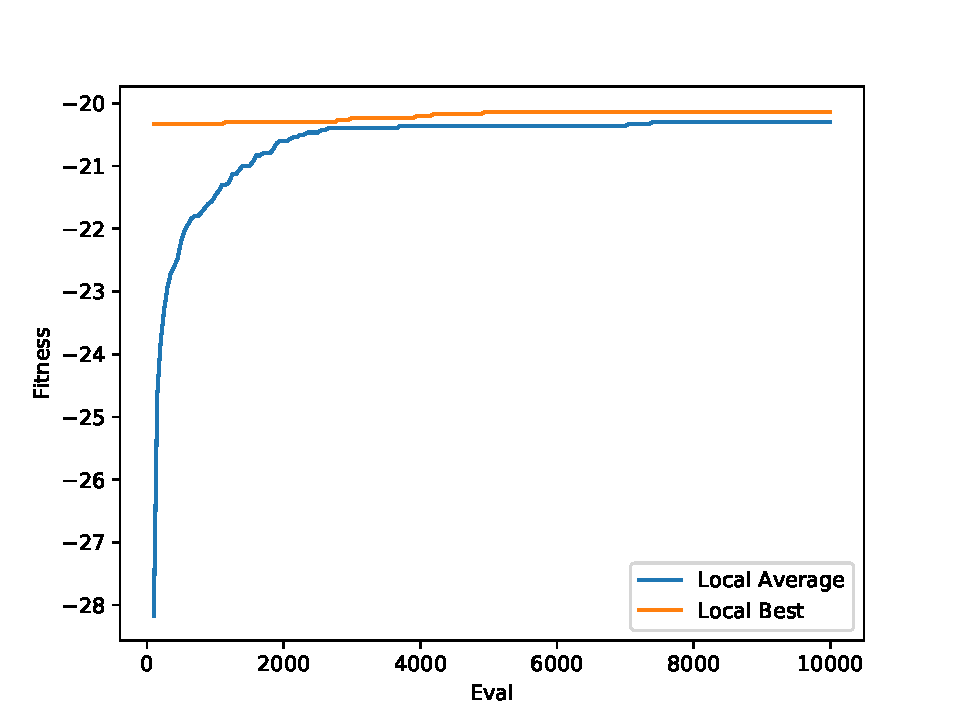
\includegraphics[width=\textwidth]{../graphs/graphs/1037.pdf}
\end{figure}


\begin{table}[!htb]
	\centering
	\caption{Figure \ref{fig:graph_1038} Configuration File}
	\label{tab:graph_1038}
	\begin{tabular}{| c | c |}
		\hline
		Self Adaptive Offspring Count		& True		 \\
		\hline
		Tournament Size For Parent Selection		& 5		 \\
		\hline
		Penalty Coefficient		& 1		 \\
		\hline
		Runs		& 30		 \\
		\hline
		Parent Selection Algorithm		& k-Tournament Selection with replacement		 \\
		\hline
		Self Adaptive Mutation Rate		& True		 \\
		\hline
		Offspring Count		& 50		 \\
		\hline
		Termination Convergence Criterion		& 10000		 \\
		\hline
		Solution File Path		& None		 \\
		\hline
		Mutation Rate		& 0.1		 \\
		\hline
		Recombination Algorithm		& Partially Mapped Crossover		 \\
		\hline
		Random Seed		& 1038		 \\
		\hline
		Mutation Algorithm		& Flip		 \\
		\hline
		Tournament Size For Survival Selection		& 5		 \\
		\hline
		Placement Algorithm		& Random with Repair		 \\
		\hline
		Population Size		& 100		 \\
		\hline
		Survival Strategy		& Plus		 \\
		\hline
		Search Algorithm		& EA		 \\
		\hline
		Log File Path		& None		 \\
		\hline
		Fitness Evaluations		& 10000		 \\
		\hline
		Survivor Algorithm		& Truncation		 \\
		\hline
		Self Adaptive Penalty Coefficient		& False		 \\
		\hline
	\end{tabular}
\end{table}
\begin{figure}[!htb]
	\caption{Input 1}
	\label{fig:graph_1038}
	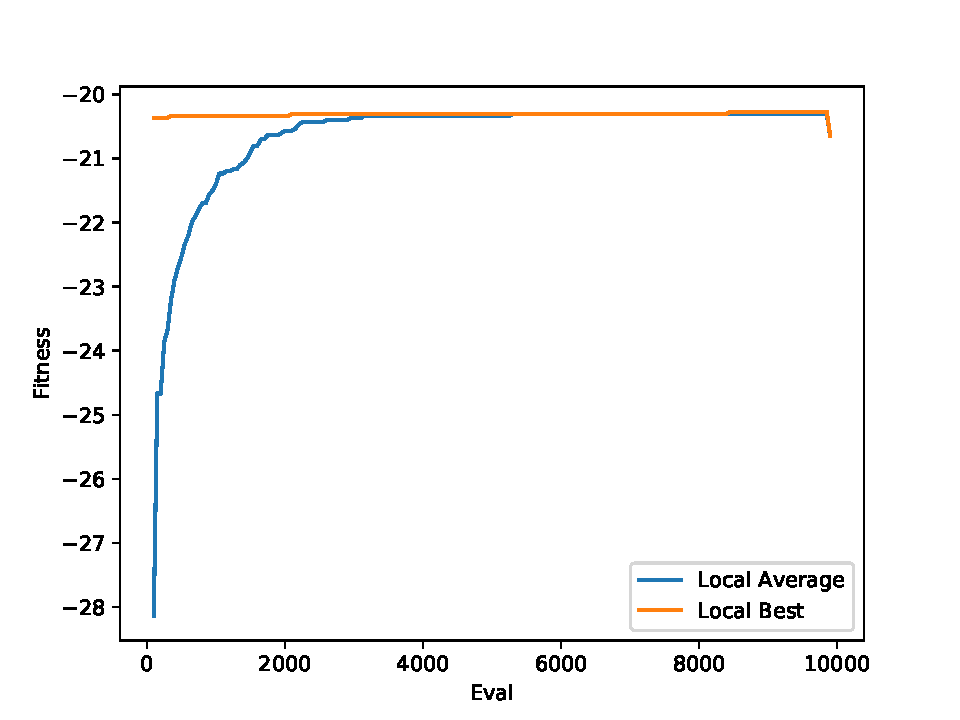
\includegraphics[width=\textwidth]{../graphs/graphs/1038.pdf}
\end{figure}


\begin{table}[!htb]
	\centering
	\caption{Figure \ref{fig:graph_1039} Configuration File}
	\label{tab:graph_1039}
	\begin{tabular}{| c | c |}
		\hline
		Self Adaptive Offspring Count		& False		 \\
		\hline
		Tournament Size For Parent Selection		& 5		 \\
		\hline
		Penalty Coefficient		& 1		 \\
		\hline
		Runs		& 30		 \\
		\hline
		Parent Selection Algorithm		& k-Tournament Selection with replacement		 \\
		\hline
		Self Adaptive Mutation Rate		& True		 \\
		\hline
		Offspring Count		& 50		 \\
		\hline
		Termination Convergence Criterion		& 10000		 \\
		\hline
		Solution File Path		& None		 \\
		\hline
		Mutation Rate		& 0.1		 \\
		\hline
		Recombination Algorithm		& Partially Mapped Crossover		 \\
		\hline
		Random Seed		& 1039		 \\
		\hline
		Mutation Algorithm		& Flip		 \\
		\hline
		Tournament Size For Survival Selection		& 5		 \\
		\hline
		Placement Algorithm		& Random with Repair		 \\
		\hline
		Population Size		& 100		 \\
		\hline
		Survival Strategy		& Plus		 \\
		\hline
		Search Algorithm		& EA		 \\
		\hline
		Log File Path		& None		 \\
		\hline
		Fitness Evaluations		& 10000		 \\
		\hline
		Survivor Algorithm		& Truncation		 \\
		\hline
		Self Adaptive Penalty Coefficient		& True		 \\
		\hline
	\end{tabular}
\end{table}
\begin{figure}[!htb]
	\caption{Input 1}
	\label{fig:graph_1039}
	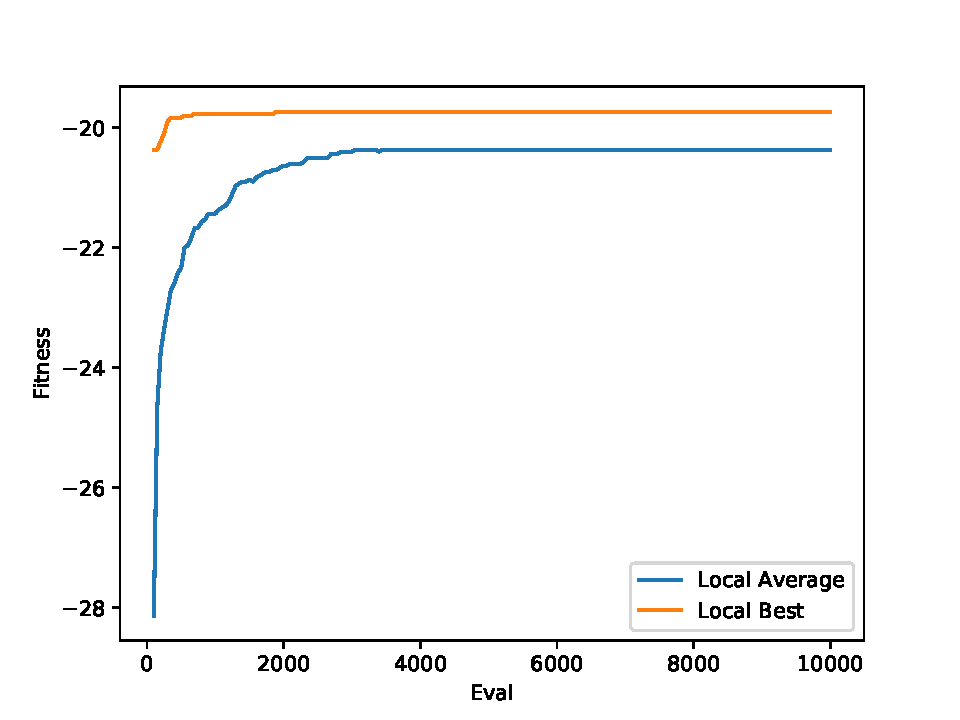
\includegraphics[width=\textwidth]{../graphs/graphs/1039.pdf}
\end{figure}


\begin{table}[!htb]
	\centering
	\caption{Figure \ref{fig:graph_1040} Configuration File}
	\label{tab:graph_1040}
	\begin{tabular}{| c | c |}
		\hline
		Self Adaptive Offspring Count		& True		 \\
		\hline
		Tournament Size For Parent Selection		& 5		 \\
		\hline
		Penalty Coefficient		& 1		 \\
		\hline
		Runs		& 30		 \\
		\hline
		Parent Selection Algorithm		& k-Tournament Selection with replacement		 \\
		\hline
		Self Adaptive Mutation Rate		& True		 \\
		\hline
		Offspring Count		& 50		 \\
		\hline
		Termination Convergence Criterion		& 10000		 \\
		\hline
		Solution File Path		& None		 \\
		\hline
		Mutation Rate		& 0.1		 \\
		\hline
		Recombination Algorithm		& Partially Mapped Crossover		 \\
		\hline
		Random Seed		& 1040		 \\
		\hline
		Mutation Algorithm		& Flip		 \\
		\hline
		Tournament Size For Survival Selection		& 5		 \\
		\hline
		Placement Algorithm		& Random with Repair		 \\
		\hline
		Population Size		& 100		 \\
		\hline
		Survival Strategy		& Plus		 \\
		\hline
		Search Algorithm		& EA		 \\
		\hline
		Log File Path		& None		 \\
		\hline
		Fitness Evaluations		& 10000		 \\
		\hline
		Survivor Algorithm		& Truncation		 \\
		\hline
		Self Adaptive Penalty Coefficient		& True		 \\
		\hline
	\end{tabular}
\end{table}
\begin{figure}[!htb]
	\caption{Input 1}
	\label{fig:graph_1040}
	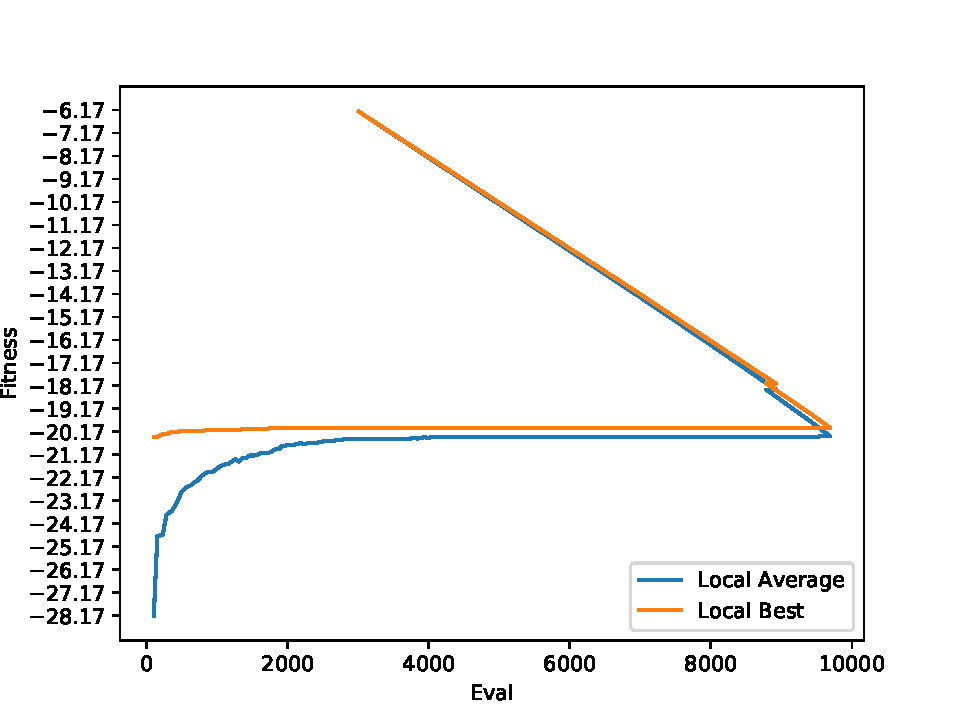
\includegraphics[width=\textwidth]{../graphs/graphs/1040.pdf}
\end{figure}


\clearpage
\begin{table}[!htb]
	\centering
	\caption{Figure \ref{fig:graph_1041} Configuration File}
	\label{tab:graph_1041}
	\begin{tabular}{| c | c |}
		\hline
		Self Adaptive Offspring Count		& False		 \\
		\hline
		Tournament Size For Parent Selection		& 5		 \\
		\hline
		Penalty Coefficient		& 1		 \\
		\hline
		Runs		& 30		 \\
		\hline
		Parent Selection Algorithm		& k-Tournament Selection with replacement		 \\
		\hline
		Self Adaptive Mutation Rate		& False		 \\
		\hline
		Offspring Count		& 50		 \\
		\hline
		Termination Convergence Criterion		& 10000		 \\
		\hline
		Solution File Path		& None		 \\
		\hline
		Mutation Rate		& 0.1		 \\
		\hline
		Recombination Algorithm		& Partially Mapped Crossover		 \\
		\hline
		Random Seed		& 1041		 \\
		\hline
		Mutation Algorithm		& Flip		 \\
		\hline
		Tournament Size For Survival Selection		& 5		 \\
		\hline
		Placement Algorithm		& Random with Penalty		 \\
		\hline
		Population Size		& 100		 \\
		\hline
		Survival Strategy		& Plus		 \\
		\hline
		Search Algorithm		& EA		 \\
		\hline
		Log File Path		& None		 \\
		\hline
		Fitness Evaluations		& 10000		 \\
		\hline
		Survivor Algorithm		& Truncation		 \\
		\hline
		Self Adaptive Penalty Coefficient		& False		 \\
		\hline
	\end{tabular}
\end{table}
\begin{figure}[!htb]
	\caption{Input 1}
	\label{fig:graph_1041}
	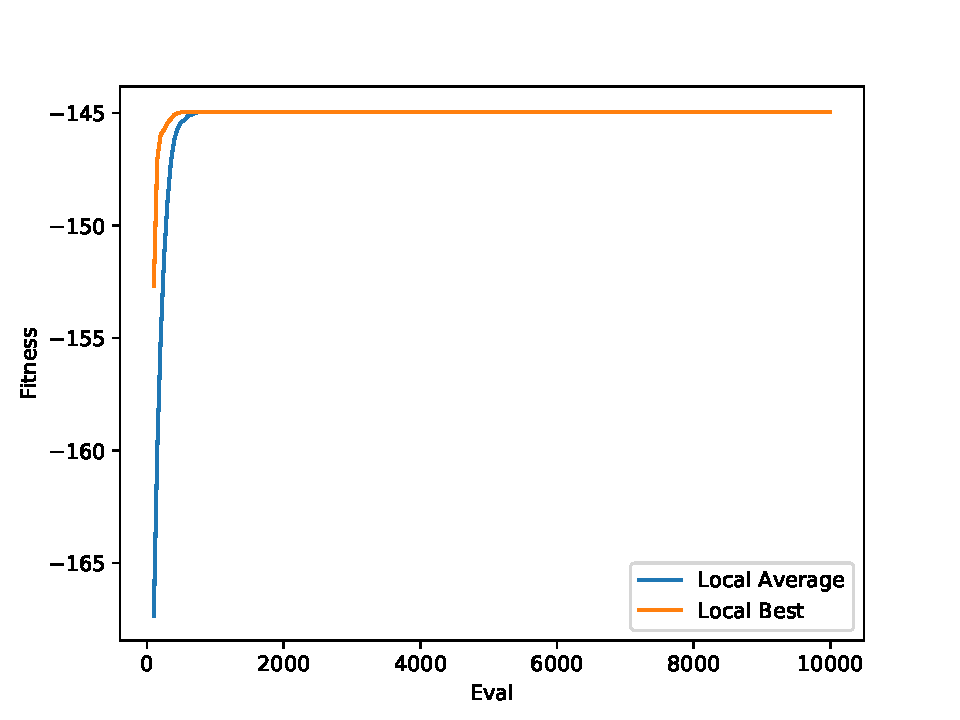
\includegraphics[width=\textwidth]{../graphs/graphs/1041.pdf}
\end{figure}


\begin{table}[!htb]
	\centering
	\caption{Figure \ref{fig:graph_1042} Configuration File}
	\label{tab:graph_1042}
	\begin{tabular}{| c | c |}
		\hline
		Self Adaptive Offspring Count		& True		 \\
		\hline
		Tournament Size For Parent Selection		& 5		 \\
		\hline
		Penalty Coefficient		& 1		 \\
		\hline
		Runs		& 30		 \\
		\hline
		Parent Selection Algorithm		& k-Tournament Selection with replacement		 \\
		\hline
		Self Adaptive Mutation Rate		& False		 \\
		\hline
		Offspring Count		& 50		 \\
		\hline
		Termination Convergence Criterion		& 10000		 \\
		\hline
		Solution File Path		& None		 \\
		\hline
		Mutation Rate		& 0.1		 \\
		\hline
		Recombination Algorithm		& Partially Mapped Crossover		 \\
		\hline
		Random Seed		& 1042		 \\
		\hline
		Mutation Algorithm		& Flip		 \\
		\hline
		Tournament Size For Survival Selection		& 5		 \\
		\hline
		Placement Algorithm		& Random with Penalty		 \\
		\hline
		Population Size		& 100		 \\
		\hline
		Survival Strategy		& Plus		 \\
		\hline
		Search Algorithm		& EA		 \\
		\hline
		Log File Path		& None		 \\
		\hline
		Fitness Evaluations		& 10000		 \\
		\hline
		Survivor Algorithm		& Truncation		 \\
		\hline
		Self Adaptive Penalty Coefficient		& False		 \\
		\hline
	\end{tabular}
\end{table}
\begin{figure}[!htb]
	\caption{Input 1}
	\label{fig:graph_1042}
	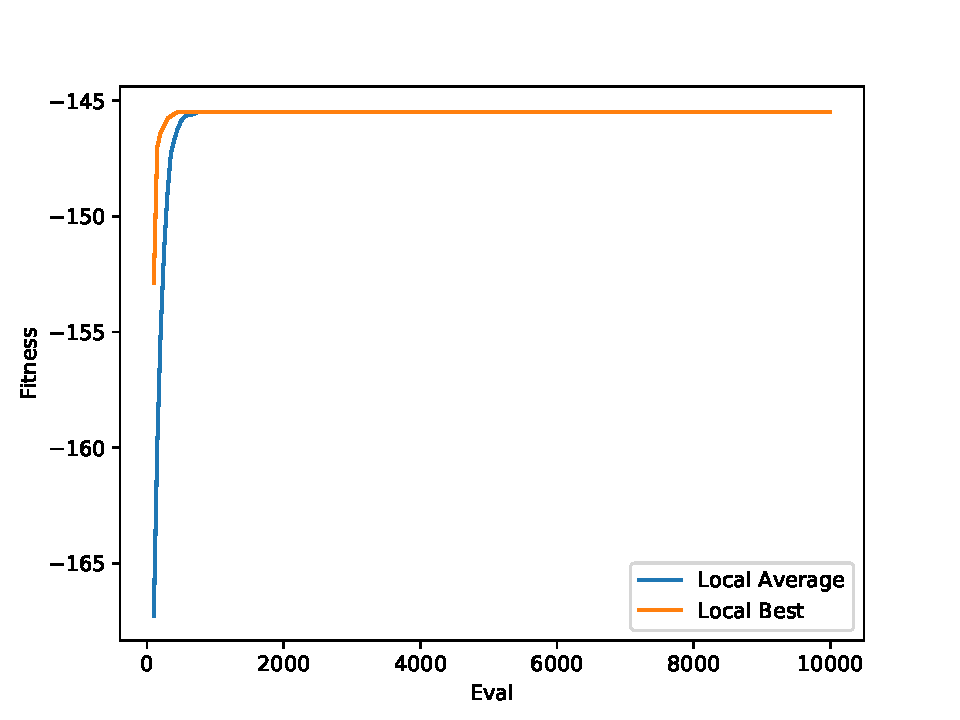
\includegraphics[width=\textwidth]{../graphs/graphs/1042.pdf}
\end{figure}


\begin{table}[!htb]
	\centering
	\caption{Figure \ref{fig:graph_1043} Configuration File}
	\label{tab:graph_1043}
	\begin{tabular}{| c | c |}
		\hline
		Self Adaptive Offspring Count		& False		 \\
		\hline
		Tournament Size For Parent Selection		& 5		 \\
		\hline
		Penalty Coefficient		& 1		 \\
		\hline
		Runs		& 30		 \\
		\hline
		Parent Selection Algorithm		& k-Tournament Selection with replacement		 \\
		\hline
		Self Adaptive Mutation Rate		& False		 \\
		\hline
		Offspring Count		& 50		 \\
		\hline
		Termination Convergence Criterion		& 10000		 \\
		\hline
		Solution File Path		& None		 \\
		\hline
		Mutation Rate		& 0.1		 \\
		\hline
		Recombination Algorithm		& Partially Mapped Crossover		 \\
		\hline
		Random Seed		& 1043		 \\
		\hline
		Mutation Algorithm		& Flip		 \\
		\hline
		Tournament Size For Survival Selection		& 5		 \\
		\hline
		Placement Algorithm		& Random with Penalty		 \\
		\hline
		Population Size		& 100		 \\
		\hline
		Survival Strategy		& Plus		 \\
		\hline
		Search Algorithm		& EA		 \\
		\hline
		Log File Path		& None		 \\
		\hline
		Fitness Evaluations		& 10000		 \\
		\hline
		Survivor Algorithm		& Truncation		 \\
		\hline
		Self Adaptive Penalty Coefficient		& True		 \\
		\hline
	\end{tabular}
\end{table}
\begin{figure}[!htb]
	\caption{Input 1}
	\label{fig:graph_1043}
	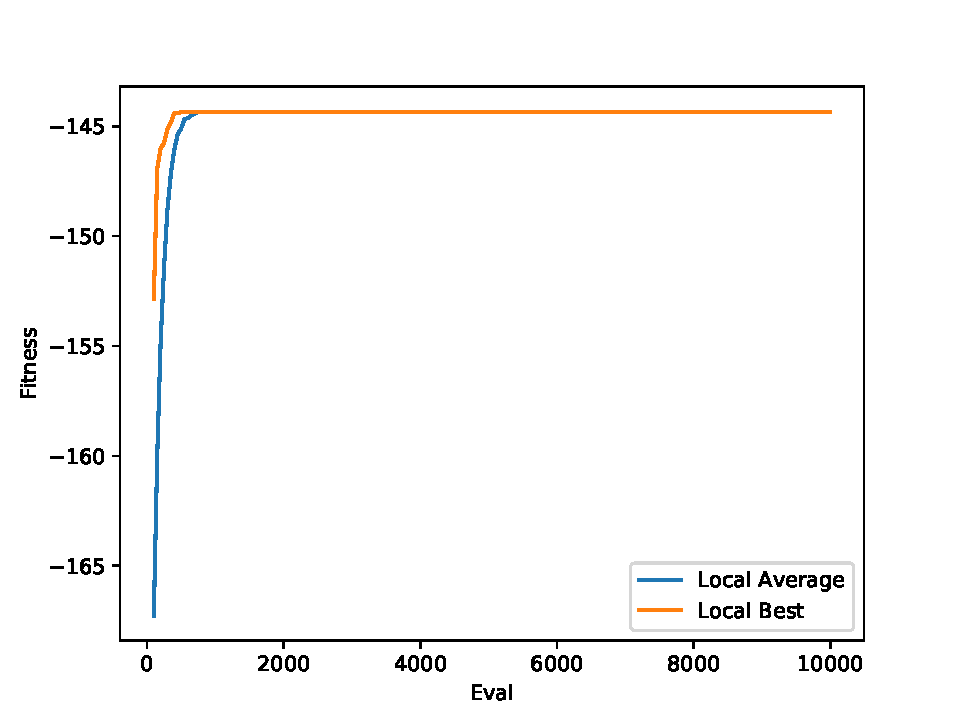
\includegraphics[width=\textwidth]{../graphs/graphs/1043.pdf}
\end{figure}


\begin{table}[!htb]
	\centering
	\caption{Figure \ref{fig:graph_1044} Configuration File}
	\label{tab:graph_1044}
	\begin{tabular}{| c | c |}
		\hline
		Self Adaptive Offspring Count		& True		 \\
		\hline
		Tournament Size For Parent Selection		& 5		 \\
		\hline
		Penalty Coefficient		& 1		 \\
		\hline
		Runs		& 30		 \\
		\hline
		Parent Selection Algorithm		& k-Tournament Selection with replacement		 \\
		\hline
		Self Adaptive Mutation Rate		& False		 \\
		\hline
		Offspring Count		& 50		 \\
		\hline
		Termination Convergence Criterion		& 10000		 \\
		\hline
		Solution File Path		& None		 \\
		\hline
		Mutation Rate		& 0.1		 \\
		\hline
		Recombination Algorithm		& Partially Mapped Crossover		 \\
		\hline
		Random Seed		& 1044		 \\
		\hline
		Mutation Algorithm		& Flip		 \\
		\hline
		Tournament Size For Survival Selection		& 5		 \\
		\hline
		Placement Algorithm		& Random with Penalty		 \\
		\hline
		Population Size		& 100		 \\
		\hline
		Survival Strategy		& Plus		 \\
		\hline
		Search Algorithm		& EA		 \\
		\hline
		Log File Path		& None		 \\
		\hline
		Fitness Evaluations		& 10000		 \\
		\hline
		Survivor Algorithm		& Truncation		 \\
		\hline
		Self Adaptive Penalty Coefficient		& True		 \\
		\hline
	\end{tabular}
\end{table}
\begin{figure}[!htb]
	\caption{Input 1}
	\label{fig:graph_1044}
	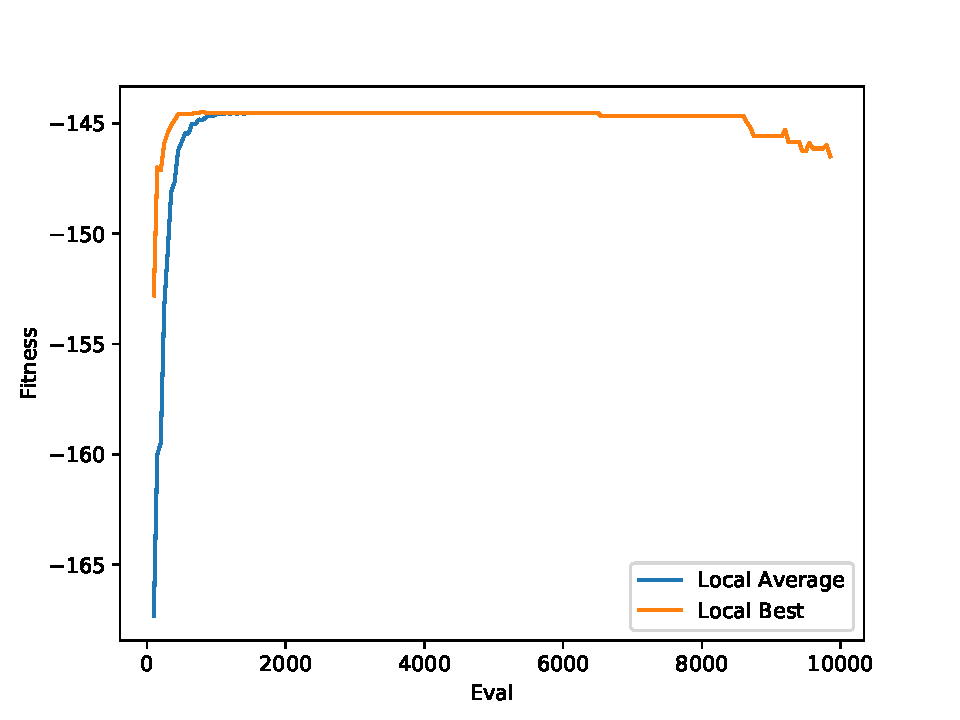
\includegraphics[width=\textwidth]{../graphs/graphs/1044.pdf}
\end{figure}


\begin{table}[!htb]
	\centering
	\caption{Figure \ref{fig:graph_1045} Configuration File}
	\label{tab:graph_1045}
	\begin{tabular}{| c | c |}
		\hline
		Self Adaptive Offspring Count		& False		 \\
		\hline
		Tournament Size For Parent Selection		& 5		 \\
		\hline
		Penalty Coefficient		& 1		 \\
		\hline
		Runs		& 30		 \\
		\hline
		Parent Selection Algorithm		& k-Tournament Selection with replacement		 \\
		\hline
		Self Adaptive Mutation Rate		& True		 \\
		\hline
		Offspring Count		& 50		 \\
		\hline
		Termination Convergence Criterion		& 10000		 \\
		\hline
		Solution File Path		& None		 \\
		\hline
		Mutation Rate		& 0.1		 \\
		\hline
		Recombination Algorithm		& Partially Mapped Crossover		 \\
		\hline
		Random Seed		& 1045		 \\
		\hline
		Mutation Algorithm		& Flip		 \\
		\hline
		Tournament Size For Survival Selection		& 5		 \\
		\hline
		Placement Algorithm		& Random with Penalty		 \\
		\hline
		Population Size		& 100		 \\
		\hline
		Survival Strategy		& Plus		 \\
		\hline
		Search Algorithm		& EA		 \\
		\hline
		Log File Path		& None		 \\
		\hline
		Fitness Evaluations		& 10000		 \\
		\hline
		Survivor Algorithm		& Truncation		 \\
		\hline
		Self Adaptive Penalty Coefficient		& False		 \\
		\hline
	\end{tabular}
\end{table}
\begin{figure}[!htb]
	\caption{Input 1}
	\label{fig:graph_1045}
	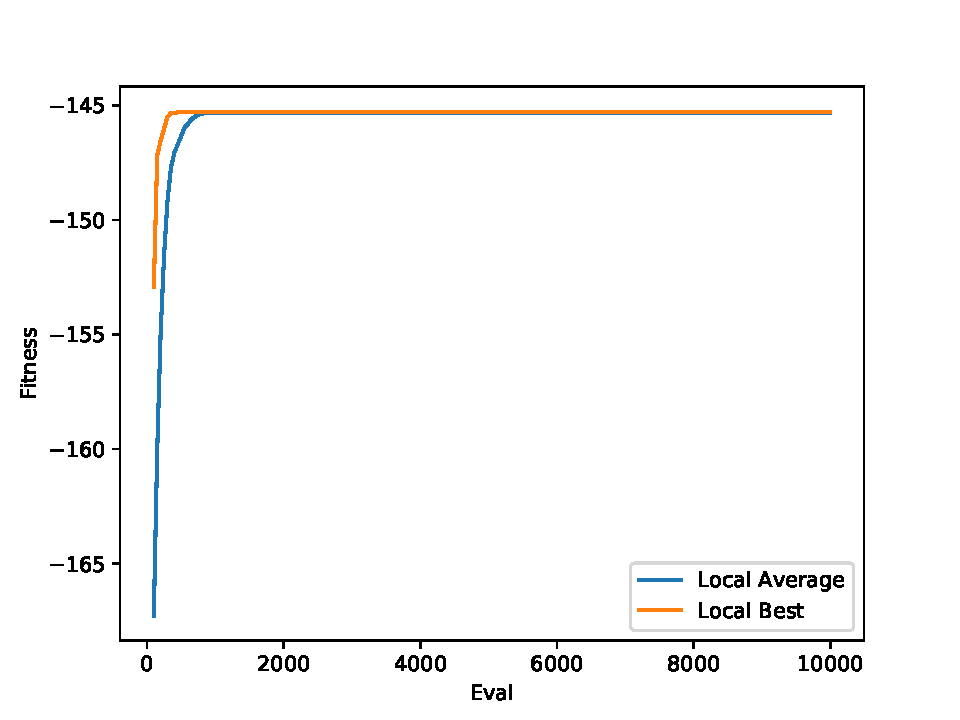
\includegraphics[width=\textwidth]{../graphs/graphs/1045.pdf}
\end{figure}


\begin{table}[!htb]
	\centering
	\caption{Figure \ref{fig:graph_1046} Configuration File}
	\label{tab:graph_1046}
	\begin{tabular}{| c | c |}
		\hline
		Self Adaptive Offspring Count		& True		 \\
		\hline
		Tournament Size For Parent Selection		& 5		 \\
		\hline
		Penalty Coefficient		& 1		 \\
		\hline
		Runs		& 30		 \\
		\hline
		Parent Selection Algorithm		& k-Tournament Selection with replacement		 \\
		\hline
		Self Adaptive Mutation Rate		& True		 \\
		\hline
		Offspring Count		& 50		 \\
		\hline
		Termination Convergence Criterion		& 10000		 \\
		\hline
		Solution File Path		& None		 \\
		\hline
		Mutation Rate		& 0.1		 \\
		\hline
		Recombination Algorithm		& Partially Mapped Crossover		 \\
		\hline
		Random Seed		& 1046		 \\
		\hline
		Mutation Algorithm		& Flip		 \\
		\hline
		Tournament Size For Survival Selection		& 5		 \\
		\hline
		Placement Algorithm		& Random with Penalty		 \\
		\hline
		Population Size		& 100		 \\
		\hline
		Survival Strategy		& Plus		 \\
		\hline
		Search Algorithm		& EA		 \\
		\hline
		Log File Path		& None		 \\
		\hline
		Fitness Evaluations		& 10000		 \\
		\hline
		Survivor Algorithm		& Truncation		 \\
		\hline
		Self Adaptive Penalty Coefficient		& False		 \\
		\hline
	\end{tabular}
\end{table}
\begin{figure}[!htb]
	\caption{Input 1}
	\label{fig:graph_1046}
	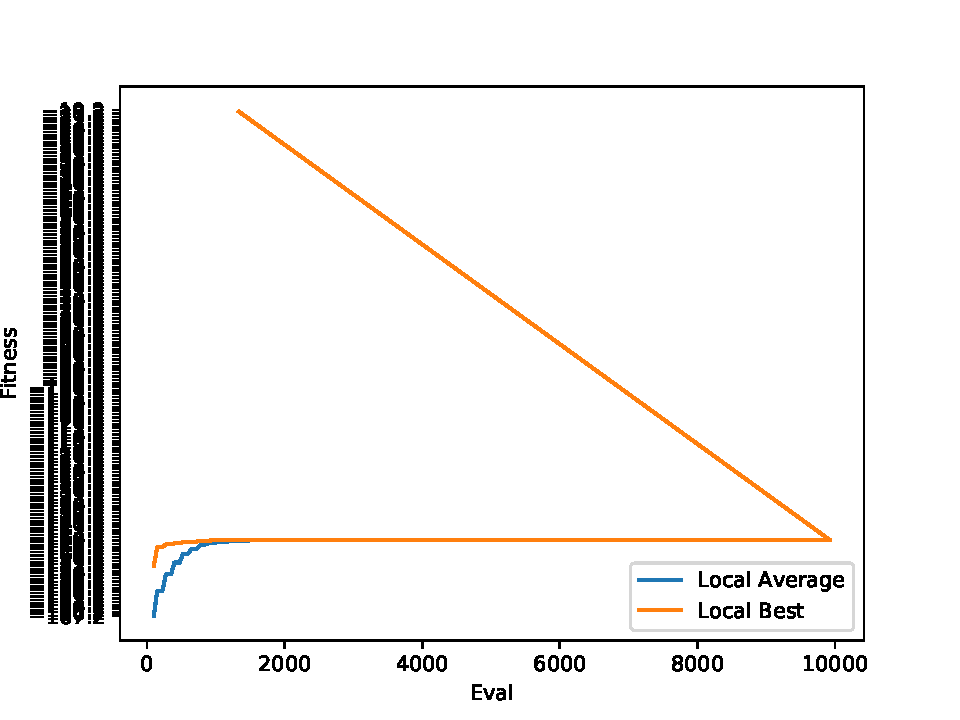
\includegraphics[width=\textwidth]{../graphs/graphs/1046.pdf}
\end{figure}


\begin{table}[!htb]
	\centering
	\caption{Figure \ref{fig:graph_1047} Configuration File}
	\label{tab:graph_1047}
	\begin{tabular}{| c | c |}
		\hline
		Self Adaptive Offspring Count		& False		 \\
		\hline
		Tournament Size For Parent Selection		& 5		 \\
		\hline
		Penalty Coefficient		& 1		 \\
		\hline
		Runs		& 30		 \\
		\hline
		Parent Selection Algorithm		& k-Tournament Selection with replacement		 \\
		\hline
		Self Adaptive Mutation Rate		& True		 \\
		\hline
		Offspring Count		& 50		 \\
		\hline
		Termination Convergence Criterion		& 10000		 \\
		\hline
		Solution File Path		& None		 \\
		\hline
		Mutation Rate		& 0.1		 \\
		\hline
		Recombination Algorithm		& Partially Mapped Crossover		 \\
		\hline
		Random Seed		& 1047		 \\
		\hline
		Mutation Algorithm		& Flip		 \\
		\hline
		Tournament Size For Survival Selection		& 5		 \\
		\hline
		Placement Algorithm		& Random with Penalty		 \\
		\hline
		Population Size		& 100		 \\
		\hline
		Survival Strategy		& Plus		 \\
		\hline
		Search Algorithm		& EA		 \\
		\hline
		Log File Path		& None		 \\
		\hline
		Fitness Evaluations		& 10000		 \\
		\hline
		Survivor Algorithm		& Truncation		 \\
		\hline
		Self Adaptive Penalty Coefficient		& True		 \\
		\hline
	\end{tabular}
\end{table}
\begin{figure}[!htb]
	\caption{Input 1}
	\label{fig:graph_1047}
	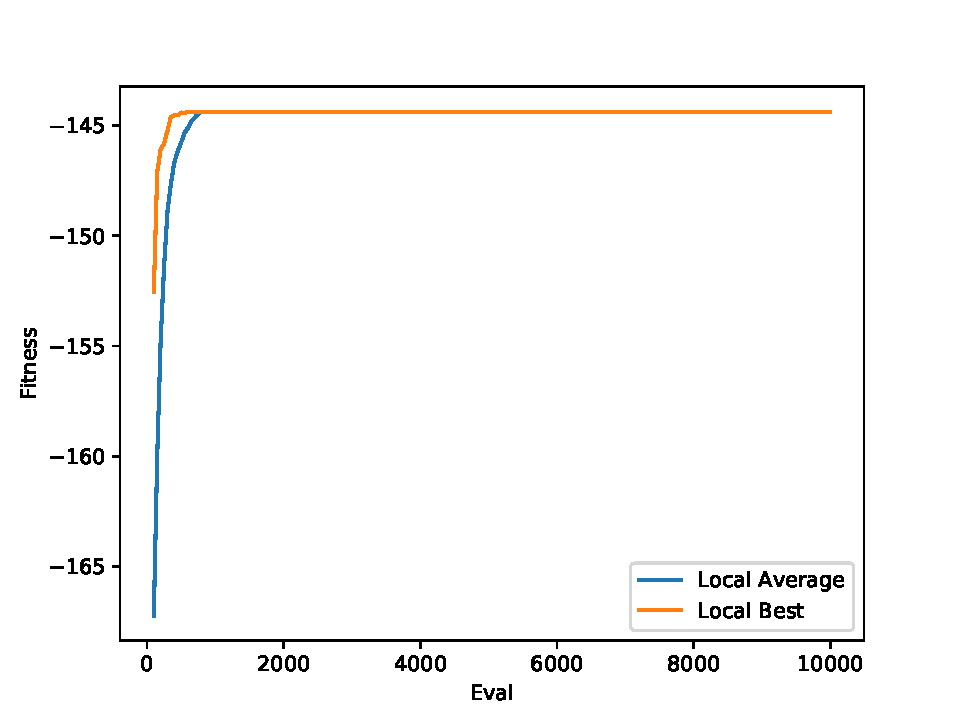
\includegraphics[width=\textwidth]{../graphs/graphs/1047.pdf}
\end{figure}


\begin{table}[!htb]
	\centering
	\caption{Figure \ref{fig:graph_1048} Configuration File}
	\label{tab:graph_1048}
	\begin{tabular}{| c | c |}
		\hline
		Self Adaptive Offspring Count		& True		 \\
		\hline
		Tournament Size For Parent Selection		& 5		 \\
		\hline
		Penalty Coefficient		& 1		 \\
		\hline
		Runs		& 30		 \\
		\hline
		Parent Selection Algorithm		& k-Tournament Selection with replacement		 \\
		\hline
		Self Adaptive Mutation Rate		& True		 \\
		\hline
		Offspring Count		& 50		 \\
		\hline
		Termination Convergence Criterion		& 10000		 \\
		\hline
		Solution File Path		& None		 \\
		\hline
		Mutation Rate		& 0.1		 \\
		\hline
		Recombination Algorithm		& Partially Mapped Crossover		 \\
		\hline
		Random Seed		& 1048		 \\
		\hline
		Mutation Algorithm		& Flip		 \\
		\hline
		Tournament Size For Survival Selection		& 5		 \\
		\hline
		Placement Algorithm		& Random with Penalty		 \\
		\hline
		Population Size		& 100		 \\
		\hline
		Survival Strategy		& Plus		 \\
		\hline
		Search Algorithm		& EA		 \\
		\hline
		Log File Path		& None		 \\
		\hline
		Fitness Evaluations		& 10000		 \\
		\hline
		Survivor Algorithm		& Truncation		 \\
		\hline
		Self Adaptive Penalty Coefficient		& True		 \\
		\hline
	\end{tabular}
\end{table}
\begin{figure}[!htb]
	\caption{Input 1}
	\label{fig:graph_1048}
	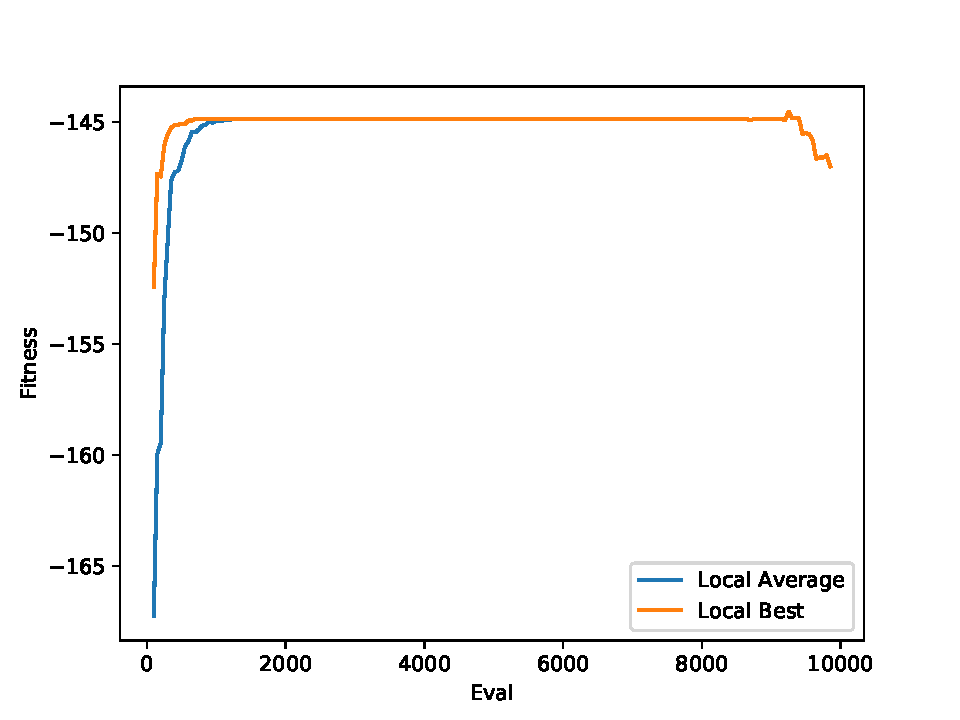
\includegraphics[width=\textwidth]{../graphs/graphs/1048.pdf}
\end{figure}


\begin{table}[!htb]
	\centering
	\caption{Figure \ref{fig:graph_1049} Configuration File}
	\label{tab:graph_1049}
	\begin{tabular}{| c | c |}
		\hline
		Self Adaptive Offspring Count		& False		 \\
		\hline
		Tournament Size For Parent Selection		& 5		 \\
		\hline
		Penalty Coefficient		& 1		 \\
		\hline
		Runs		& 30		 \\
		\hline
		Parent Selection Algorithm		& k-Tournament Selection with replacement		 \\
		\hline
		Self Adaptive Mutation Rate		& False		 \\
		\hline
		Offspring Count		& 50		 \\
		\hline
		Termination Convergence Criterion		& 10000		 \\
		\hline
		Solution File Path		& None		 \\
		\hline
		Mutation Rate		& 0.1		 \\
		\hline
		Recombination Algorithm		& Order Crossover		 \\
		\hline
		Random Seed		& 1049		 \\
		\hline
		Mutation Algorithm		& Flip		 \\
		\hline
		Tournament Size For Survival Selection		& 5		 \\
		\hline
		Placement Algorithm		& Random		 \\
		\hline
		Population Size		& 100		 \\
		\hline
		Survival Strategy		& Plus		 \\
		\hline
		Search Algorithm		& EA		 \\
		\hline
		Log File Path		& None		 \\
		\hline
		Fitness Evaluations		& 10000		 \\
		\hline
		Survivor Algorithm		& Truncation		 \\
		\hline
		Self Adaptive Penalty Coefficient		& False		 \\
		\hline
	\end{tabular}
\end{table}
\begin{figure}[!htb]
	\caption{Input 1}
	\label{fig:graph_1049}
	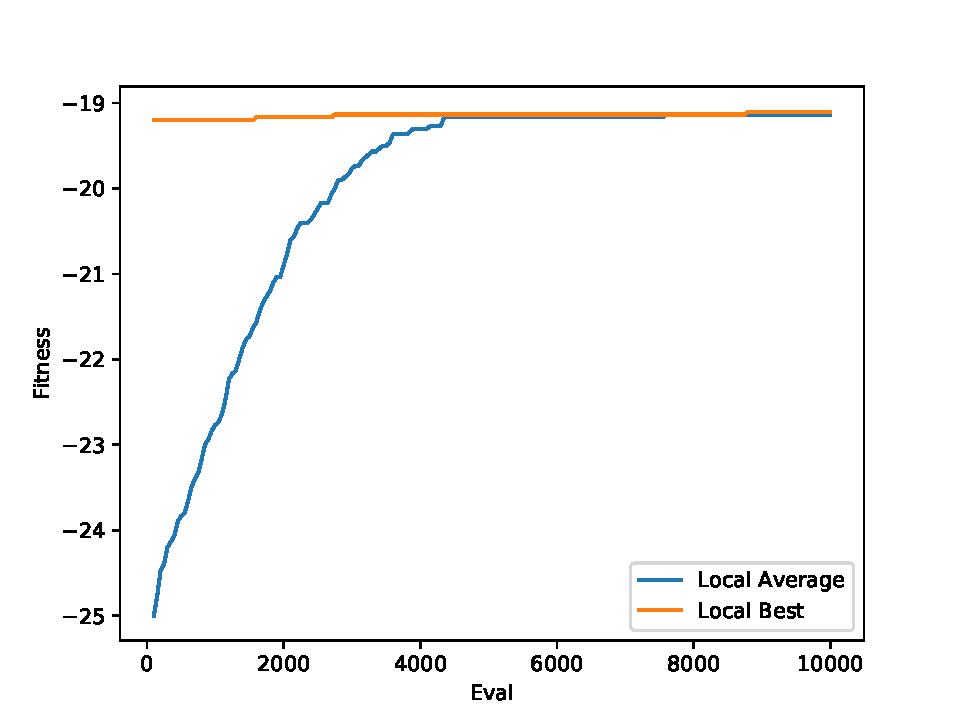
\includegraphics[width=\textwidth]{../graphs/graphs/1049.pdf}
\end{figure}


\begin{table}[!htb]
	\centering
	\caption{Figure \ref{fig:graph_1050} Configuration File}
	\label{tab:graph_1050}
	\begin{tabular}{| c | c |}
		\hline
		Self Adaptive Offspring Count		& False		 \\
		\hline
		Tournament Size For Parent Selection		& 5		 \\
		\hline
		Penalty Coefficient		& 1		 \\
		\hline
		Runs		& 30		 \\
		\hline
		Parent Selection Algorithm		& k-Tournament Selection with replacement		 \\
		\hline
		Self Adaptive Mutation Rate		& False		 \\
		\hline
		Offspring Count		& 50		 \\
		\hline
		Termination Convergence Criterion		& 10000		 \\
		\hline
		Solution File Path		& None		 \\
		\hline
		Mutation Rate		& 0.1		 \\
		\hline
		Recombination Algorithm		& Order Crossover		 \\
		\hline
		Random Seed		& 1050		 \\
		\hline
		Mutation Algorithm		& Move		 \\
		\hline
		Tournament Size For Survival Selection		& 5		 \\
		\hline
		Placement Algorithm		& Random		 \\
		\hline
		Population Size		& 100		 \\
		\hline
		Survival Strategy		& Plus		 \\
		\hline
		Search Algorithm		& EA		 \\
		\hline
		Log File Path		& None		 \\
		\hline
		Fitness Evaluations		& 10000		 \\
		\hline
		Survivor Algorithm		& Truncation		 \\
		\hline
		Self Adaptive Penalty Coefficient		& False		 \\
		\hline
	\end{tabular}
\end{table}
\begin{figure}[!htb]
	\caption{Input 1}
	\label{fig:graph_1050}
	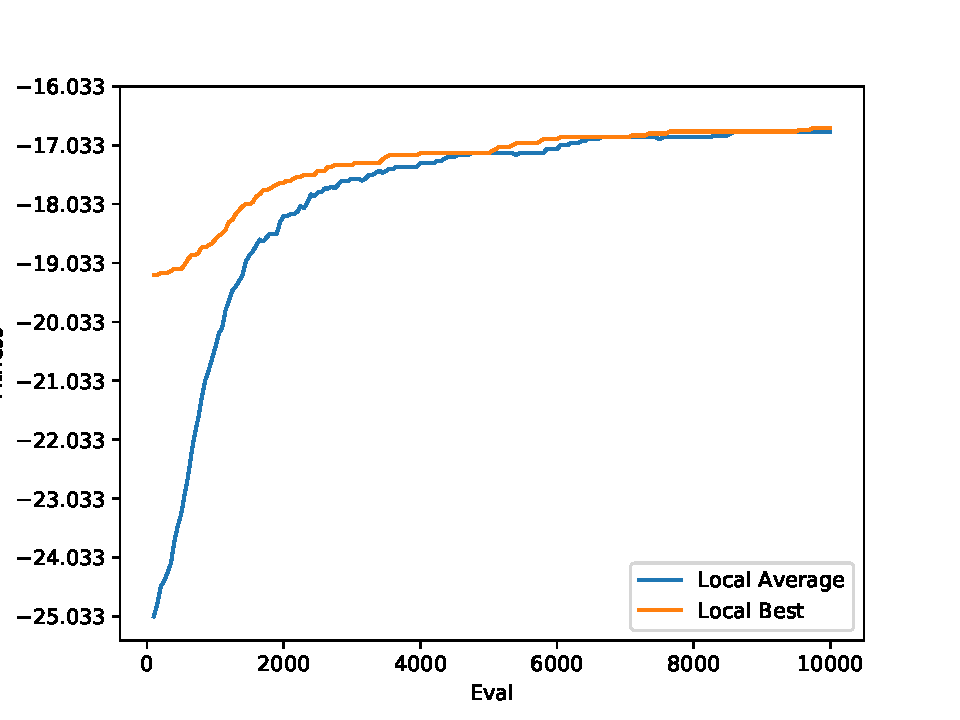
\includegraphics[width=\textwidth]{../graphs/graphs/1050.pdf}
\end{figure}


\clearpage
\begin{table}[!htb]
	\centering
	\caption{Figure \ref{fig:graph_1051} Configuration File}
	\label{tab:graph_1051}
	\begin{tabular}{| c | c |}
		\hline
		Self Adaptive Offspring Count		& True		 \\
		\hline
		Tournament Size For Parent Selection		& 5		 \\
		\hline
		Penalty Coefficient		& 1		 \\
		\hline
		Runs		& 30		 \\
		\hline
		Parent Selection Algorithm		& k-Tournament Selection with replacement		 \\
		\hline
		Self Adaptive Mutation Rate		& False		 \\
		\hline
		Offspring Count		& 50		 \\
		\hline
		Termination Convergence Criterion		& 10000		 \\
		\hline
		Solution File Path		& None		 \\
		\hline
		Mutation Rate		& 0.1		 \\
		\hline
		Recombination Algorithm		& Order Crossover		 \\
		\hline
		Random Seed		& 1051		 \\
		\hline
		Mutation Algorithm		& Flip		 \\
		\hline
		Tournament Size For Survival Selection		& 5		 \\
		\hline
		Placement Algorithm		& Random		 \\
		\hline
		Population Size		& 100		 \\
		\hline
		Survival Strategy		& Plus		 \\
		\hline
		Search Algorithm		& EA		 \\
		\hline
		Log File Path		& None		 \\
		\hline
		Fitness Evaluations		& 10000		 \\
		\hline
		Survivor Algorithm		& Truncation		 \\
		\hline
		Self Adaptive Penalty Coefficient		& False		 \\
		\hline
	\end{tabular}
\end{table}
\begin{figure}[!htb]
	\caption{Input 1}
	\label{fig:graph_1051}
	\includegraphics[width=\textwidth]{../graphs/graphs/1051.pdf}
\end{figure}


\begin{table}[!htb]
	\centering
	\caption{Figure \ref{fig:graph_1052} Configuration File}
	\label{tab:graph_1052}
	\begin{tabular}{| c | c |}
		\hline
		Self Adaptive Offspring Count		& True		 \\
		\hline
		Tournament Size For Parent Selection		& 5		 \\
		\hline
		Penalty Coefficient		& 1		 \\
		\hline
		Runs		& 30		 \\
		\hline
		Parent Selection Algorithm		& k-Tournament Selection with replacement		 \\
		\hline
		Self Adaptive Mutation Rate		& False		 \\
		\hline
		Offspring Count		& 50		 \\
		\hline
		Termination Convergence Criterion		& 10000		 \\
		\hline
		Solution File Path		& None		 \\
		\hline
		Mutation Rate		& 0.1		 \\
		\hline
		Recombination Algorithm		& Order Crossover		 \\
		\hline
		Random Seed		& 1052		 \\
		\hline
		Mutation Algorithm		& Move		 \\
		\hline
		Tournament Size For Survival Selection		& 5		 \\
		\hline
		Placement Algorithm		& Random		 \\
		\hline
		Population Size		& 100		 \\
		\hline
		Survival Strategy		& Plus		 \\
		\hline
		Search Algorithm		& EA		 \\
		\hline
		Log File Path		& None		 \\
		\hline
		Fitness Evaluations		& 10000		 \\
		\hline
		Survivor Algorithm		& Truncation		 \\
		\hline
		Self Adaptive Penalty Coefficient		& False		 \\
		\hline
	\end{tabular}
\end{table}
\begin{figure}[!htb]
	\caption{Input 1}
	\label{fig:graph_1052}
	\includegraphics[width=\textwidth]{../graphs/graphs/1052.pdf}
\end{figure}


\begin{table}[!htb]
	\centering
	\caption{Figure \ref{fig:graph_1053} Configuration File}
	\label{tab:graph_1053}
	\begin{tabular}{| c | c |}
		\hline
		Self Adaptive Offspring Count		& False		 \\
		\hline
		Tournament Size For Parent Selection		& 5		 \\
		\hline
		Penalty Coefficient		& 1		 \\
		\hline
		Runs		& 30		 \\
		\hline
		Parent Selection Algorithm		& k-Tournament Selection with replacement		 \\
		\hline
		Self Adaptive Mutation Rate		& True		 \\
		\hline
		Offspring Count		& 50		 \\
		\hline
		Termination Convergence Criterion		& 10000		 \\
		\hline
		Solution File Path		& None		 \\
		\hline
		Mutation Rate		& 0.1		 \\
		\hline
		Recombination Algorithm		& Order Crossover		 \\
		\hline
		Random Seed		& 1053		 \\
		\hline
		Mutation Algorithm		& Flip		 \\
		\hline
		Tournament Size For Survival Selection		& 5		 \\
		\hline
		Placement Algorithm		& Random		 \\
		\hline
		Population Size		& 100		 \\
		\hline
		Survival Strategy		& Plus		 \\
		\hline
		Search Algorithm		& EA		 \\
		\hline
		Log File Path		& None		 \\
		\hline
		Fitness Evaluations		& 10000		 \\
		\hline
		Survivor Algorithm		& Truncation		 \\
		\hline
		Self Adaptive Penalty Coefficient		& False		 \\
		\hline
	\end{tabular}
\end{table}
\begin{figure}[!htb]
	\caption{Input 1}
	\label{fig:graph_1053}
	\includegraphics[width=\textwidth]{../graphs/graphs/1053.pdf}
\end{figure}


\begin{table}[!htb]
	\centering
	\caption{Figure \ref{fig:graph_1054} Configuration File}
	\label{tab:graph_1054}
	\begin{tabular}{| c | c |}
		\hline
		Self Adaptive Offspring Count		& False		 \\
		\hline
		Tournament Size For Parent Selection		& 5		 \\
		\hline
		Penalty Coefficient		& 1		 \\
		\hline
		Runs		& 30		 \\
		\hline
		Parent Selection Algorithm		& k-Tournament Selection with replacement		 \\
		\hline
		Self Adaptive Mutation Rate		& True		 \\
		\hline
		Offspring Count		& 50		 \\
		\hline
		Termination Convergence Criterion		& 10000		 \\
		\hline
		Solution File Path		& None		 \\
		\hline
		Mutation Rate		& 0.1		 \\
		\hline
		Recombination Algorithm		& Order Crossover		 \\
		\hline
		Random Seed		& 1054		 \\
		\hline
		Mutation Algorithm		& Move		 \\
		\hline
		Tournament Size For Survival Selection		& 5		 \\
		\hline
		Placement Algorithm		& Random		 \\
		\hline
		Population Size		& 100		 \\
		\hline
		Survival Strategy		& Plus		 \\
		\hline
		Search Algorithm		& EA		 \\
		\hline
		Log File Path		& None		 \\
		\hline
		Fitness Evaluations		& 10000		 \\
		\hline
		Survivor Algorithm		& Truncation		 \\
		\hline
		Self Adaptive Penalty Coefficient		& False		 \\
		\hline
	\end{tabular}
\end{table}
\begin{figure}[!htb]
	\caption{Input 1}
	\label{fig:graph_1054}
	\includegraphics[width=\textwidth]{../graphs/graphs/1054.pdf}
\end{figure}


\begin{table}[!htb]
	\centering
	\caption{Figure \ref{fig:graph_1055} Configuration File}
	\label{tab:graph_1055}
	\begin{tabular}{| c | c |}
		\hline
		Self Adaptive Offspring Count		& True		 \\
		\hline
		Tournament Size For Parent Selection		& 5		 \\
		\hline
		Penalty Coefficient		& 1		 \\
		\hline
		Runs		& 30		 \\
		\hline
		Parent Selection Algorithm		& k-Tournament Selection with replacement		 \\
		\hline
		Self Adaptive Mutation Rate		& True		 \\
		\hline
		Offspring Count		& 50		 \\
		\hline
		Termination Convergence Criterion		& 10000		 \\
		\hline
		Solution File Path		& None		 \\
		\hline
		Mutation Rate		& 0.1		 \\
		\hline
		Recombination Algorithm		& Order Crossover		 \\
		\hline
		Random Seed		& 1055		 \\
		\hline
		Mutation Algorithm		& Flip		 \\
		\hline
		Tournament Size For Survival Selection		& 5		 \\
		\hline
		Placement Algorithm		& Random		 \\
		\hline
		Population Size		& 100		 \\
		\hline
		Survival Strategy		& Plus		 \\
		\hline
		Search Algorithm		& EA		 \\
		\hline
		Log File Path		& None		 \\
		\hline
		Fitness Evaluations		& 10000		 \\
		\hline
		Survivor Algorithm		& Truncation		 \\
		\hline
		Self Adaptive Penalty Coefficient		& False		 \\
		\hline
	\end{tabular}
\end{table}
\begin{figure}[!htb]
	\caption{Input 1}
	\label{fig:graph_1055}
	\includegraphics[width=\textwidth]{../graphs/graphs/1055.pdf}
\end{figure}


\begin{table}[!htb]
	\centering
	\caption{Figure \ref{fig:graph_1056} Configuration File}
	\label{tab:graph_1056}
	\begin{tabular}{| c | c |}
		\hline
		Self Adaptive Offspring Count		& True		 \\
		\hline
		Tournament Size For Parent Selection		& 5		 \\
		\hline
		Penalty Coefficient		& 1		 \\
		\hline
		Runs		& 30		 \\
		\hline
		Parent Selection Algorithm		& k-Tournament Selection with replacement		 \\
		\hline
		Self Adaptive Mutation Rate		& True		 \\
		\hline
		Offspring Count		& 50		 \\
		\hline
		Termination Convergence Criterion		& 10000		 \\
		\hline
		Solution File Path		& None		 \\
		\hline
		Mutation Rate		& 0.1		 \\
		\hline
		Recombination Algorithm		& Order Crossover		 \\
		\hline
		Random Seed		& 1056		 \\
		\hline
		Mutation Algorithm		& Move		 \\
		\hline
		Tournament Size For Survival Selection		& 5		 \\
		\hline
		Placement Algorithm		& Random		 \\
		\hline
		Population Size		& 100		 \\
		\hline
		Survival Strategy		& Plus		 \\
		\hline
		Search Algorithm		& EA		 \\
		\hline
		Log File Path		& None		 \\
		\hline
		Fitness Evaluations		& 10000		 \\
		\hline
		Survivor Algorithm		& Truncation		 \\
		\hline
		Self Adaptive Penalty Coefficient		& False		 \\
		\hline
	\end{tabular}
\end{table}
\begin{figure}[!htb]
	\caption{Input 1}
	\label{fig:graph_1056}
	\includegraphics[width=\textwidth]{../graphs/graphs/1056.pdf}
\end{figure}


\begin{table}[!htb]
	\centering
	\caption{Figure \ref{fig:graph_1057} Configuration File}
	\label{tab:graph_1057}
	\begin{tabular}{| c | c |}
		\hline
		Self Adaptive Offspring Count		& False		 \\
		\hline
		Tournament Size For Parent Selection		& 5		 \\
		\hline
		Penalty Coefficient		& 1		 \\
		\hline
		Runs		& 30		 \\
		\hline
		Parent Selection Algorithm		& k-Tournament Selection with replacement		 \\
		\hline
		Self Adaptive Mutation Rate		& False		 \\
		\hline
		Offspring Count		& 50		 \\
		\hline
		Termination Convergence Criterion		& 10000		 \\
		\hline
		Solution File Path		& None		 \\
		\hline
		Mutation Rate		& 0.1		 \\
		\hline
		Recombination Algorithm		& Order Crossover		 \\
		\hline
		Random Seed		& 1057		 \\
		\hline
		Mutation Algorithm		& Flip		 \\
		\hline
		Tournament Size For Survival Selection		& 5		 \\
		\hline
		Placement Algorithm		& Random with Repair		 \\
		\hline
		Population Size		& 100		 \\
		\hline
		Survival Strategy		& Plus		 \\
		\hline
		Search Algorithm		& EA		 \\
		\hline
		Log File Path		& None		 \\
		\hline
		Fitness Evaluations		& 10000		 \\
		\hline
		Survivor Algorithm		& Truncation		 \\
		\hline
		Self Adaptive Penalty Coefficient		& False		 \\
		\hline
	\end{tabular}
\end{table}
\begin{figure}[!htb]
	\caption{Input 1}
	\label{fig:graph_1057}
	\includegraphics[width=\textwidth]{../graphs/graphs/1057.pdf}
\end{figure}


\begin{table}[!htb]
	\centering
	\caption{Figure \ref{fig:graph_1058} Configuration File}
	\label{tab:graph_1058}
	\begin{tabular}{| c | c |}
		\hline
		Self Adaptive Offspring Count		& False		 \\
		\hline
		Tournament Size For Parent Selection		& 5		 \\
		\hline
		Penalty Coefficient		& 1		 \\
		\hline
		Runs		& 30		 \\
		\hline
		Parent Selection Algorithm		& k-Tournament Selection with replacement		 \\
		\hline
		Self Adaptive Mutation Rate		& False		 \\
		\hline
		Offspring Count		& 50		 \\
		\hline
		Termination Convergence Criterion		& 10000		 \\
		\hline
		Solution File Path		& None		 \\
		\hline
		Mutation Rate		& 0.1		 \\
		\hline
		Recombination Algorithm		& Order Crossover		 \\
		\hline
		Random Seed		& 1058		 \\
		\hline
		Mutation Algorithm		& Move		 \\
		\hline
		Tournament Size For Survival Selection		& 5		 \\
		\hline
		Placement Algorithm		& Random with Repair		 \\
		\hline
		Population Size		& 100		 \\
		\hline
		Survival Strategy		& Plus		 \\
		\hline
		Search Algorithm		& EA		 \\
		\hline
		Log File Path		& None		 \\
		\hline
		Fitness Evaluations		& 10000		 \\
		\hline
		Survivor Algorithm		& Truncation		 \\
		\hline
		Self Adaptive Penalty Coefficient		& False		 \\
		\hline
	\end{tabular}
\end{table}
\begin{figure}[!htb]
	\caption{Input 1}
	\label{fig:graph_1058}
	\includegraphics[width=\textwidth]{../graphs/graphs/1058.pdf}
\end{figure}


\begin{table}[!htb]
	\centering
	\caption{Figure \ref{fig:graph_1059} Configuration File}
	\label{tab:graph_1059}
	\begin{tabular}{| c | c |}
		\hline
		Self Adaptive Offspring Count		& True		 \\
		\hline
		Tournament Size For Parent Selection		& 5		 \\
		\hline
		Penalty Coefficient		& 1		 \\
		\hline
		Runs		& 30		 \\
		\hline
		Parent Selection Algorithm		& k-Tournament Selection with replacement		 \\
		\hline
		Self Adaptive Mutation Rate		& False		 \\
		\hline
		Offspring Count		& 50		 \\
		\hline
		Termination Convergence Criterion		& 10000		 \\
		\hline
		Solution File Path		& None		 \\
		\hline
		Mutation Rate		& 0.1		 \\
		\hline
		Recombination Algorithm		& Order Crossover		 \\
		\hline
		Random Seed		& 1059		 \\
		\hline
		Mutation Algorithm		& Flip		 \\
		\hline
		Tournament Size For Survival Selection		& 5		 \\
		\hline
		Placement Algorithm		& Random with Repair		 \\
		\hline
		Population Size		& 100		 \\
		\hline
		Survival Strategy		& Plus		 \\
		\hline
		Search Algorithm		& EA		 \\
		\hline
		Log File Path		& None		 \\
		\hline
		Fitness Evaluations		& 10000		 \\
		\hline
		Survivor Algorithm		& Truncation		 \\
		\hline
		Self Adaptive Penalty Coefficient		& False		 \\
		\hline
	\end{tabular}
\end{table}
\begin{figure}[!htb]
	\caption{Input 1}
	\label{fig:graph_1059}
	\includegraphics[width=\textwidth]{../graphs/graphs/1059.pdf}
\end{figure}


\begin{table}[!htb]
	\centering
	\caption{Figure \ref{fig:graph_1060} Configuration File}
	\label{tab:graph_1060}
	\begin{tabular}{| c | c |}
		\hline
		Self Adaptive Offspring Count		& True		 \\
		\hline
		Tournament Size For Parent Selection		& 5		 \\
		\hline
		Penalty Coefficient		& 1		 \\
		\hline
		Runs		& 30		 \\
		\hline
		Parent Selection Algorithm		& k-Tournament Selection with replacement		 \\
		\hline
		Self Adaptive Mutation Rate		& False		 \\
		\hline
		Offspring Count		& 50		 \\
		\hline
		Termination Convergence Criterion		& 10000		 \\
		\hline
		Solution File Path		& None		 \\
		\hline
		Mutation Rate		& 0.1		 \\
		\hline
		Recombination Algorithm		& Order Crossover		 \\
		\hline
		Random Seed		& 1060		 \\
		\hline
		Mutation Algorithm		& Move		 \\
		\hline
		Tournament Size For Survival Selection		& 5		 \\
		\hline
		Placement Algorithm		& Random with Repair		 \\
		\hline
		Population Size		& 100		 \\
		\hline
		Survival Strategy		& Plus		 \\
		\hline
		Search Algorithm		& EA		 \\
		\hline
		Log File Path		& None		 \\
		\hline
		Fitness Evaluations		& 10000		 \\
		\hline
		Survivor Algorithm		& Truncation		 \\
		\hline
		Self Adaptive Penalty Coefficient		& False		 \\
		\hline
	\end{tabular}
\end{table}
\begin{figure}[!htb]
	\caption{Input 1}
	\label{fig:graph_1060}
	\includegraphics[width=\textwidth]{../graphs/graphs/1060.pdf}
\end{figure}


\clearpage
\begin{table}[!htb]
	\centering
	\caption{Figure \ref{fig:graph_1061} Configuration File}
	\label{tab:graph_1061}
	\begin{tabular}{| c | c |}
		\hline
		Self Adaptive Offspring Count		& False		 \\
		\hline
		Tournament Size For Parent Selection		& 5		 \\
		\hline
		Penalty Coefficient		& 1		 \\
		\hline
		Runs		& 30		 \\
		\hline
		Parent Selection Algorithm		& k-Tournament Selection with replacement		 \\
		\hline
		Self Adaptive Mutation Rate		& True		 \\
		\hline
		Offspring Count		& 50		 \\
		\hline
		Termination Convergence Criterion		& 10000		 \\
		\hline
		Solution File Path		& None		 \\
		\hline
		Mutation Rate		& 0.1		 \\
		\hline
		Recombination Algorithm		& Order Crossover		 \\
		\hline
		Random Seed		& 1061		 \\
		\hline
		Mutation Algorithm		& Flip		 \\
		\hline
		Tournament Size For Survival Selection		& 5		 \\
		\hline
		Placement Algorithm		& Random with Repair		 \\
		\hline
		Population Size		& 100		 \\
		\hline
		Survival Strategy		& Plus		 \\
		\hline
		Search Algorithm		& EA		 \\
		\hline
		Log File Path		& None		 \\
		\hline
		Fitness Evaluations		& 10000		 \\
		\hline
		Survivor Algorithm		& Truncation		 \\
		\hline
		Self Adaptive Penalty Coefficient		& False		 \\
		\hline
	\end{tabular}
\end{table}
\begin{figure}[!htb]
	\caption{Input 1}
	\label{fig:graph_1061}
	\includegraphics[width=\textwidth]{../graphs/graphs/1061.pdf}
\end{figure}


\begin{table}[!htb]
	\centering
	\caption{Figure \ref{fig:graph_1062} Configuration File}
	\label{tab:graph_1062}
	\begin{tabular}{| c | c |}
		\hline
		Self Adaptive Offspring Count		& False		 \\
		\hline
		Tournament Size For Parent Selection		& 5		 \\
		\hline
		Penalty Coefficient		& 1		 \\
		\hline
		Runs		& 30		 \\
		\hline
		Parent Selection Algorithm		& k-Tournament Selection with replacement		 \\
		\hline
		Self Adaptive Mutation Rate		& True		 \\
		\hline
		Offspring Count		& 50		 \\
		\hline
		Termination Convergence Criterion		& 10000		 \\
		\hline
		Solution File Path		& None		 \\
		\hline
		Mutation Rate		& 0.1		 \\
		\hline
		Recombination Algorithm		& Order Crossover		 \\
		\hline
		Random Seed		& 1062		 \\
		\hline
		Mutation Algorithm		& Move		 \\
		\hline
		Tournament Size For Survival Selection		& 5		 \\
		\hline
		Placement Algorithm		& Random with Repair		 \\
		\hline
		Population Size		& 100		 \\
		\hline
		Survival Strategy		& Plus		 \\
		\hline
		Search Algorithm		& EA		 \\
		\hline
		Log File Path		& None		 \\
		\hline
		Fitness Evaluations		& 10000		 \\
		\hline
		Survivor Algorithm		& Truncation		 \\
		\hline
		Self Adaptive Penalty Coefficient		& False		 \\
		\hline
	\end{tabular}
\end{table}
\begin{figure}[!htb]
	\caption{Input 1}
	\label{fig:graph_1062}
	\includegraphics[width=\textwidth]{../graphs/graphs/1062.pdf}
\end{figure}


\begin{table}[!htb]
	\centering
	\caption{Figure \ref{fig:graph_1063} Configuration File}
	\label{tab:graph_1063}
	\begin{tabular}{| c | c |}
		\hline
		Self Adaptive Offspring Count		& True		 \\
		\hline
		Tournament Size For Parent Selection		& 5		 \\
		\hline
		Penalty Coefficient		& 1		 \\
		\hline
		Runs		& 30		 \\
		\hline
		Parent Selection Algorithm		& k-Tournament Selection with replacement		 \\
		\hline
		Self Adaptive Mutation Rate		& True		 \\
		\hline
		Offspring Count		& 50		 \\
		\hline
		Termination Convergence Criterion		& 10000		 \\
		\hline
		Solution File Path		& None		 \\
		\hline
		Mutation Rate		& 0.1		 \\
		\hline
		Recombination Algorithm		& Order Crossover		 \\
		\hline
		Random Seed		& 1063		 \\
		\hline
		Mutation Algorithm		& Flip		 \\
		\hline
		Tournament Size For Survival Selection		& 5		 \\
		\hline
		Placement Algorithm		& Random with Repair		 \\
		\hline
		Population Size		& 100		 \\
		\hline
		Survival Strategy		& Plus		 \\
		\hline
		Search Algorithm		& EA		 \\
		\hline
		Log File Path		& None		 \\
		\hline
		Fitness Evaluations		& 10000		 \\
		\hline
		Survivor Algorithm		& Truncation		 \\
		\hline
		Self Adaptive Penalty Coefficient		& False		 \\
		\hline
	\end{tabular}
\end{table}
\begin{figure}[!htb]
	\caption{Input 1}
	\label{fig:graph_1063}
	\includegraphics[width=\textwidth]{../graphs/graphs/1063.pdf}
\end{figure}


\begin{table}[!htb]
	\centering
	\caption{Figure \ref{fig:graph_1064} Configuration File}
	\label{tab:graph_1064}
	\begin{tabular}{| c | c |}
		\hline
		Self Adaptive Offspring Count		& True		 \\
		\hline
		Tournament Size For Parent Selection		& 5		 \\
		\hline
		Penalty Coefficient		& 1		 \\
		\hline
		Runs		& 30		 \\
		\hline
		Parent Selection Algorithm		& k-Tournament Selection with replacement		 \\
		\hline
		Self Adaptive Mutation Rate		& True		 \\
		\hline
		Offspring Count		& 50		 \\
		\hline
		Termination Convergence Criterion		& 10000		 \\
		\hline
		Solution File Path		& None		 \\
		\hline
		Mutation Rate		& 0.1		 \\
		\hline
		Recombination Algorithm		& Order Crossover		 \\
		\hline
		Random Seed		& 1064		 \\
		\hline
		Mutation Algorithm		& Move		 \\
		\hline
		Tournament Size For Survival Selection		& 5		 \\
		\hline
		Placement Algorithm		& Random with Repair		 \\
		\hline
		Population Size		& 100		 \\
		\hline
		Survival Strategy		& Plus		 \\
		\hline
		Search Algorithm		& EA		 \\
		\hline
		Log File Path		& None		 \\
		\hline
		Fitness Evaluations		& 10000		 \\
		\hline
		Survivor Algorithm		& Truncation		 \\
		\hline
		Self Adaptive Penalty Coefficient		& False		 \\
		\hline
	\end{tabular}
\end{table}
\begin{figure}[!htb]
	\caption{Input 1}
	\label{fig:graph_1064}
	\includegraphics[width=\textwidth]{../graphs/graphs/1064.pdf}
\end{figure}


\begin{table}[!htb]
	\centering
	\caption{Figure \ref{fig:graph_1065} Configuration File}
	\label{tab:graph_1065}
	\begin{tabular}{| c | c |}
		\hline
		Self Adaptive Offspring Count		& False		 \\
		\hline
		Tournament Size For Parent Selection		& 5		 \\
		\hline
		Penalty Coefficient		& 1		 \\
		\hline
		Runs		& 30		 \\
		\hline
		Parent Selection Algorithm		& k-Tournament Selection with replacement		 \\
		\hline
		Self Adaptive Mutation Rate		& False		 \\
		\hline
		Offspring Count		& 50		 \\
		\hline
		Termination Convergence Criterion		& 10000		 \\
		\hline
		Solution File Path		& None		 \\
		\hline
		Mutation Rate		& 0.1		 \\
		\hline
		Recombination Algorithm		& Order Crossover		 \\
		\hline
		Random Seed		& 1065		 \\
		\hline
		Mutation Algorithm		& Flip		 \\
		\hline
		Tournament Size For Survival Selection		& 5		 \\
		\hline
		Placement Algorithm		& Random with Penalty		 \\
		\hline
		Population Size		& 100		 \\
		\hline
		Survival Strategy		& Plus		 \\
		\hline
		Search Algorithm		& EA		 \\
		\hline
		Log File Path		& None		 \\
		\hline
		Fitness Evaluations		& 10000		 \\
		\hline
		Survivor Algorithm		& Truncation		 \\
		\hline
		Self Adaptive Penalty Coefficient		& False		 \\
		\hline
	\end{tabular}
\end{table}
\begin{figure}[!htb]
	\caption{Input 1}
	\label{fig:graph_1065}
	\includegraphics[width=\textwidth]{../graphs/graphs/1065.pdf}
\end{figure}


\begin{table}[!htb]
	\centering
	\caption{Figure \ref{fig:graph_1066} Configuration File}
	\label{tab:graph_1066}
	\begin{tabular}{| c | c |}
		\hline
		Self Adaptive Offspring Count		& False		 \\
		\hline
		Tournament Size For Parent Selection		& 5		 \\
		\hline
		Penalty Coefficient		& 1		 \\
		\hline
		Runs		& 30		 \\
		\hline
		Parent Selection Algorithm		& k-Tournament Selection with replacement		 \\
		\hline
		Self Adaptive Mutation Rate		& False		 \\
		\hline
		Offspring Count		& 50		 \\
		\hline
		Termination Convergence Criterion		& 10000		 \\
		\hline
		Solution File Path		& None		 \\
		\hline
		Mutation Rate		& 0.1		 \\
		\hline
		Recombination Algorithm		& Order Crossover		 \\
		\hline
		Random Seed		& 1066		 \\
		\hline
		Mutation Algorithm		& Move		 \\
		\hline
		Tournament Size For Survival Selection		& 5		 \\
		\hline
		Placement Algorithm		& Random with Penalty		 \\
		\hline
		Population Size		& 100		 \\
		\hline
		Survival Strategy		& Plus		 \\
		\hline
		Search Algorithm		& EA		 \\
		\hline
		Log File Path		& None		 \\
		\hline
		Fitness Evaluations		& 10000		 \\
		\hline
		Survivor Algorithm		& Truncation		 \\
		\hline
		Self Adaptive Penalty Coefficient		& False		 \\
		\hline
	\end{tabular}
\end{table}
\begin{figure}[!htb]
	\caption{Input 1}
	\label{fig:graph_1066}
	\includegraphics[width=\textwidth]{../graphs/graphs/1066.pdf}
\end{figure}


\begin{table}[!htb]
	\centering
	\caption{Figure \ref{fig:graph_1067} Configuration File}
	\label{tab:graph_1067}
	\begin{tabular}{| c | c |}
		\hline
		Self Adaptive Offspring Count		& True		 \\
		\hline
		Tournament Size For Parent Selection		& 5		 \\
		\hline
		Penalty Coefficient		& 1		 \\
		\hline
		Runs		& 30		 \\
		\hline
		Parent Selection Algorithm		& k-Tournament Selection with replacement		 \\
		\hline
		Self Adaptive Mutation Rate		& False		 \\
		\hline
		Offspring Count		& 50		 \\
		\hline
		Termination Convergence Criterion		& 10000		 \\
		\hline
		Solution File Path		& None		 \\
		\hline
		Mutation Rate		& 0.1		 \\
		\hline
		Recombination Algorithm		& Order Crossover		 \\
		\hline
		Random Seed		& 1067		 \\
		\hline
		Mutation Algorithm		& Flip		 \\
		\hline
		Tournament Size For Survival Selection		& 5		 \\
		\hline
		Placement Algorithm		& Random with Penalty		 \\
		\hline
		Population Size		& 100		 \\
		\hline
		Survival Strategy		& Plus		 \\
		\hline
		Search Algorithm		& EA		 \\
		\hline
		Log File Path		& None		 \\
		\hline
		Fitness Evaluations		& 10000		 \\
		\hline
		Survivor Algorithm		& Truncation		 \\
		\hline
		Self Adaptive Penalty Coefficient		& False		 \\
		\hline
	\end{tabular}
\end{table}
\begin{figure}[!htb]
	\caption{Input 1}
	\label{fig:graph_1067}
	\includegraphics[width=\textwidth]{../graphs/graphs/1067.pdf}
\end{figure}


\begin{table}[!htb]
	\centering
	\caption{Figure \ref{fig:graph_1068} Configuration File}
	\label{tab:graph_1068}
	\begin{tabular}{| c | c |}
		\hline
		Self Adaptive Offspring Count		& True		 \\
		\hline
		Tournament Size For Parent Selection		& 5		 \\
		\hline
		Penalty Coefficient		& 1		 \\
		\hline
		Runs		& 30		 \\
		\hline
		Parent Selection Algorithm		& k-Tournament Selection with replacement		 \\
		\hline
		Self Adaptive Mutation Rate		& False		 \\
		\hline
		Offspring Count		& 50		 \\
		\hline
		Termination Convergence Criterion		& 10000		 \\
		\hline
		Solution File Path		& None		 \\
		\hline
		Mutation Rate		& 0.1		 \\
		\hline
		Recombination Algorithm		& Order Crossover		 \\
		\hline
		Random Seed		& 1068		 \\
		\hline
		Mutation Algorithm		& Move		 \\
		\hline
		Tournament Size For Survival Selection		& 5		 \\
		\hline
		Placement Algorithm		& Random with Penalty		 \\
		\hline
		Population Size		& 100		 \\
		\hline
		Survival Strategy		& Plus		 \\
		\hline
		Search Algorithm		& EA		 \\
		\hline
		Log File Path		& None		 \\
		\hline
		Fitness Evaluations		& 10000		 \\
		\hline
		Survivor Algorithm		& Truncation		 \\
		\hline
		Self Adaptive Penalty Coefficient		& False		 \\
		\hline
	\end{tabular}
\end{table}
\begin{figure}[!htb]
	\caption{Input 1}
	\label{fig:graph_1068}
	\includegraphics[width=\textwidth]{../graphs/graphs/1068.pdf}
\end{figure}


\begin{table}[!htb]
	\centering
	\caption{Figure \ref{fig:graph_1069} Configuration File}
	\label{tab:graph_1069}
	\begin{tabular}{| c | c |}
		\hline
		Self Adaptive Offspring Count		& False		 \\
		\hline
		Tournament Size For Parent Selection		& 5		 \\
		\hline
		Penalty Coefficient		& 1		 \\
		\hline
		Runs		& 30		 \\
		\hline
		Parent Selection Algorithm		& k-Tournament Selection with replacement		 \\
		\hline
		Self Adaptive Mutation Rate		& False		 \\
		\hline
		Offspring Count		& 50		 \\
		\hline
		Termination Convergence Criterion		& 10000		 \\
		\hline
		Solution File Path		& None		 \\
		\hline
		Mutation Rate		& 0.1		 \\
		\hline
		Recombination Algorithm		& Order Crossover		 \\
		\hline
		Random Seed		& 1069		 \\
		\hline
		Mutation Algorithm		& Flip		 \\
		\hline
		Tournament Size For Survival Selection		& 5		 \\
		\hline
		Placement Algorithm		& Random with Penalty		 \\
		\hline
		Population Size		& 100		 \\
		\hline
		Survival Strategy		& Plus		 \\
		\hline
		Search Algorithm		& EA		 \\
		\hline
		Log File Path		& None		 \\
		\hline
		Fitness Evaluations		& 10000		 \\
		\hline
		Survivor Algorithm		& Truncation		 \\
		\hline
		Self Adaptive Penalty Coefficient		& True		 \\
		\hline
	\end{tabular}
\end{table}
\begin{figure}[!htb]
	\caption{Input 1}
	\label{fig:graph_1069}
	\includegraphics[width=\textwidth]{../graphs/graphs/1069.pdf}
\end{figure}


\begin{table}[!htb]
	\centering
	\caption{Figure \ref{fig:graph_1070} Configuration File}
	\label{tab:graph_1070}
	\begin{tabular}{| c | c |}
		\hline
		Self Adaptive Offspring Count		& False		 \\
		\hline
		Tournament Size For Parent Selection		& 5		 \\
		\hline
		Penalty Coefficient		& 1		 \\
		\hline
		Runs		& 30		 \\
		\hline
		Parent Selection Algorithm		& k-Tournament Selection with replacement		 \\
		\hline
		Self Adaptive Mutation Rate		& False		 \\
		\hline
		Offspring Count		& 50		 \\
		\hline
		Termination Convergence Criterion		& 10000		 \\
		\hline
		Solution File Path		& None		 \\
		\hline
		Mutation Rate		& 0.1		 \\
		\hline
		Recombination Algorithm		& Order Crossover		 \\
		\hline
		Random Seed		& 1070		 \\
		\hline
		Mutation Algorithm		& Move		 \\
		\hline
		Tournament Size For Survival Selection		& 5		 \\
		\hline
		Placement Algorithm		& Random with Penalty		 \\
		\hline
		Population Size		& 100		 \\
		\hline
		Survival Strategy		& Plus		 \\
		\hline
		Search Algorithm		& EA		 \\
		\hline
		Log File Path		& None		 \\
		\hline
		Fitness Evaluations		& 10000		 \\
		\hline
		Survivor Algorithm		& Truncation		 \\
		\hline
		Self Adaptive Penalty Coefficient		& True		 \\
		\hline
	\end{tabular}
\end{table}
\begin{figure}[!htb]
	\caption{Input 1}
	\label{fig:graph_1070}
	\includegraphics[width=\textwidth]{../graphs/graphs/1070.pdf}
\end{figure}


\clearpage
\begin{table}[!htb]
	\centering
	\caption{Figure \ref{fig:graph_1071} Configuration File}
	\label{tab:graph_1071}
	\begin{tabular}{| c | c |}
		\hline
		Self Adaptive Offspring Count		& True		 \\
		\hline
		Tournament Size For Parent Selection		& 5		 \\
		\hline
		Penalty Coefficient		& 1		 \\
		\hline
		Runs		& 30		 \\
		\hline
		Parent Selection Algorithm		& k-Tournament Selection with replacement		 \\
		\hline
		Self Adaptive Mutation Rate		& False		 \\
		\hline
		Offspring Count		& 50		 \\
		\hline
		Termination Convergence Criterion		& 10000		 \\
		\hline
		Solution File Path		& None		 \\
		\hline
		Mutation Rate		& 0.1		 \\
		\hline
		Recombination Algorithm		& Order Crossover		 \\
		\hline
		Random Seed		& 1071		 \\
		\hline
		Mutation Algorithm		& Flip		 \\
		\hline
		Tournament Size For Survival Selection		& 5		 \\
		\hline
		Placement Algorithm		& Random with Penalty		 \\
		\hline
		Population Size		& 100		 \\
		\hline
		Survival Strategy		& Plus		 \\
		\hline
		Search Algorithm		& EA		 \\
		\hline
		Log File Path		& None		 \\
		\hline
		Fitness Evaluations		& 10000		 \\
		\hline
		Survivor Algorithm		& Truncation		 \\
		\hline
		Self Adaptive Penalty Coefficient		& True		 \\
		\hline
	\end{tabular}
\end{table}
\begin{figure}[!htb]
	\caption{Input 1}
	\label{fig:graph_1071}
	\includegraphics[width=\textwidth]{../graphs/graphs/1071.pdf}
\end{figure}


\begin{table}[!htb]
	\centering
	\caption{Figure \ref{fig:graph_1072} Configuration File}
	\label{tab:graph_1072}
	\begin{tabular}{| c | c |}
		\hline
		Self Adaptive Offspring Count		& True		 \\
		\hline
		Tournament Size For Parent Selection		& 5		 \\
		\hline
		Penalty Coefficient		& 1		 \\
		\hline
		Runs		& 30		 \\
		\hline
		Parent Selection Algorithm		& k-Tournament Selection with replacement		 \\
		\hline
		Self Adaptive Mutation Rate		& False		 \\
		\hline
		Offspring Count		& 50		 \\
		\hline
		Termination Convergence Criterion		& 10000		 \\
		\hline
		Solution File Path		& None		 \\
		\hline
		Mutation Rate		& 0.1		 \\
		\hline
		Recombination Algorithm		& Order Crossover		 \\
		\hline
		Random Seed		& 1072		 \\
		\hline
		Mutation Algorithm		& Move		 \\
		\hline
		Tournament Size For Survival Selection		& 5		 \\
		\hline
		Placement Algorithm		& Random with Penalty		 \\
		\hline
		Population Size		& 100		 \\
		\hline
		Survival Strategy		& Plus		 \\
		\hline
		Search Algorithm		& EA		 \\
		\hline
		Log File Path		& None		 \\
		\hline
		Fitness Evaluations		& 10000		 \\
		\hline
		Survivor Algorithm		& Truncation		 \\
		\hline
		Self Adaptive Penalty Coefficient		& True		 \\
		\hline
	\end{tabular}
\end{table}
\begin{figure}[!htb]
	\caption{Input 1}
	\label{fig:graph_1072}
	\includegraphics[width=\textwidth]{../graphs/graphs/1072.pdf}
\end{figure}


\begin{table}[!htb]
	\centering
	\caption{Figure \ref{fig:graph_1073} Configuration File}
	\label{tab:graph_1073}
	\begin{tabular}{| c | c |}
		\hline
		Self Adaptive Offspring Count		& False		 \\
		\hline
		Tournament Size For Parent Selection		& 5		 \\
		\hline
		Penalty Coefficient		& 1		 \\
		\hline
		Runs		& 30		 \\
		\hline
		Parent Selection Algorithm		& k-Tournament Selection with replacement		 \\
		\hline
		Self Adaptive Mutation Rate		& True		 \\
		\hline
		Offspring Count		& 50		 \\
		\hline
		Termination Convergence Criterion		& 10000		 \\
		\hline
		Solution File Path		& None		 \\
		\hline
		Mutation Rate		& 0.1		 \\
		\hline
		Recombination Algorithm		& Order Crossover		 \\
		\hline
		Random Seed		& 1073		 \\
		\hline
		Mutation Algorithm		& Flip		 \\
		\hline
		Tournament Size For Survival Selection		& 5		 \\
		\hline
		Placement Algorithm		& Random with Penalty		 \\
		\hline
		Population Size		& 100		 \\
		\hline
		Survival Strategy		& Plus		 \\
		\hline
		Search Algorithm		& EA		 \\
		\hline
		Log File Path		& None		 \\
		\hline
		Fitness Evaluations		& 10000		 \\
		\hline
		Survivor Algorithm		& Truncation		 \\
		\hline
		Self Adaptive Penalty Coefficient		& False		 \\
		\hline
	\end{tabular}
\end{table}
\begin{figure}[!htb]
	\caption{Input 1}
	\label{fig:graph_1073}
	\includegraphics[width=\textwidth]{../graphs/graphs/1073.pdf}
\end{figure}


\begin{table}[!htb]
	\centering
	\caption{Figure \ref{fig:graph_1074} Configuration File}
	\label{tab:graph_1074}
	\begin{tabular}{| c | c |}
		\hline
		Self Adaptive Offspring Count		& False		 \\
		\hline
		Tournament Size For Parent Selection		& 5		 \\
		\hline
		Penalty Coefficient		& 1		 \\
		\hline
		Runs		& 30		 \\
		\hline
		Parent Selection Algorithm		& k-Tournament Selection with replacement		 \\
		\hline
		Self Adaptive Mutation Rate		& True		 \\
		\hline
		Offspring Count		& 50		 \\
		\hline
		Termination Convergence Criterion		& 10000		 \\
		\hline
		Solution File Path		& None		 \\
		\hline
		Mutation Rate		& 0.1		 \\
		\hline
		Recombination Algorithm		& Order Crossover		 \\
		\hline
		Random Seed		& 1074		 \\
		\hline
		Mutation Algorithm		& Move		 \\
		\hline
		Tournament Size For Survival Selection		& 5		 \\
		\hline
		Placement Algorithm		& Random with Penalty		 \\
		\hline
		Population Size		& 100		 \\
		\hline
		Survival Strategy		& Plus		 \\
		\hline
		Search Algorithm		& EA		 \\
		\hline
		Log File Path		& None		 \\
		\hline
		Fitness Evaluations		& 10000		 \\
		\hline
		Survivor Algorithm		& Truncation		 \\
		\hline
		Self Adaptive Penalty Coefficient		& False		 \\
		\hline
	\end{tabular}
\end{table}
\begin{figure}[!htb]
	\caption{Input 1}
	\label{fig:graph_1074}
	\includegraphics[width=\textwidth]{../graphs/graphs/1074.pdf}
\end{figure}


\begin{table}[!htb]
	\centering
	\caption{Figure \ref{fig:graph_1075} Configuration File}
	\label{tab:graph_1075}
	\begin{tabular}{| c | c |}
		\hline
		Self Adaptive Offspring Count		& True		 \\
		\hline
		Tournament Size For Parent Selection		& 5		 \\
		\hline
		Penalty Coefficient		& 1		 \\
		\hline
		Runs		& 30		 \\
		\hline
		Parent Selection Algorithm		& k-Tournament Selection with replacement		 \\
		\hline
		Self Adaptive Mutation Rate		& True		 \\
		\hline
		Offspring Count		& 50		 \\
		\hline
		Termination Convergence Criterion		& 10000		 \\
		\hline
		Solution File Path		& None		 \\
		\hline
		Mutation Rate		& 0.1		 \\
		\hline
		Recombination Algorithm		& Order Crossover		 \\
		\hline
		Random Seed		& 1075		 \\
		\hline
		Mutation Algorithm		& Flip		 \\
		\hline
		Tournament Size For Survival Selection		& 5		 \\
		\hline
		Placement Algorithm		& Random with Penalty		 \\
		\hline
		Population Size		& 100		 \\
		\hline
		Survival Strategy		& Plus		 \\
		\hline
		Search Algorithm		& EA		 \\
		\hline
		Log File Path		& None		 \\
		\hline
		Fitness Evaluations		& 10000		 \\
		\hline
		Survivor Algorithm		& Truncation		 \\
		\hline
		Self Adaptive Penalty Coefficient		& False		 \\
		\hline
	\end{tabular}
\end{table}
\begin{figure}[!htb]
	\caption{Input 1}
	\label{fig:graph_1075}
	\includegraphics[width=\textwidth]{../graphs/graphs/1075.pdf}
\end{figure}


\begin{table}[!htb]
	\centering
	\caption{Figure \ref{fig:graph_1076} Configuration File}
	\label{tab:graph_1076}
	\begin{tabular}{| c | c |}
		\hline
		Self Adaptive Offspring Count		& True		 \\
		\hline
		Tournament Size For Parent Selection		& 5		 \\
		\hline
		Penalty Coefficient		& 1		 \\
		\hline
		Runs		& 30		 \\
		\hline
		Parent Selection Algorithm		& k-Tournament Selection with replacement		 \\
		\hline
		Self Adaptive Mutation Rate		& True		 \\
		\hline
		Offspring Count		& 50		 \\
		\hline
		Termination Convergence Criterion		& 10000		 \\
		\hline
		Solution File Path		& None		 \\
		\hline
		Mutation Rate		& 0.1		 \\
		\hline
		Recombination Algorithm		& Order Crossover		 \\
		\hline
		Random Seed		& 1076		 \\
		\hline
		Mutation Algorithm		& Move		 \\
		\hline
		Tournament Size For Survival Selection		& 5		 \\
		\hline
		Placement Algorithm		& Random with Penalty		 \\
		\hline
		Population Size		& 100		 \\
		\hline
		Survival Strategy		& Plus		 \\
		\hline
		Search Algorithm		& EA		 \\
		\hline
		Log File Path		& None		 \\
		\hline
		Fitness Evaluations		& 10000		 \\
		\hline
		Survivor Algorithm		& Truncation		 \\
		\hline
		Self Adaptive Penalty Coefficient		& False		 \\
		\hline
	\end{tabular}
\end{table}
\begin{figure}[!htb]
	\caption{Input 1}
	\label{fig:graph_1076}
	\includegraphics[width=\textwidth]{../graphs/graphs/1076.pdf}
\end{figure}


\begin{table}[!htb]
	\centering
	\caption{Figure \ref{fig:graph_1077} Configuration File}
	\label{tab:graph_1077}
	\begin{tabular}{| c | c |}
		\hline
		Self Adaptive Offspring Count		& False		 \\
		\hline
		Tournament Size For Parent Selection		& 5		 \\
		\hline
		Penalty Coefficient		& 1		 \\
		\hline
		Runs		& 30		 \\
		\hline
		Parent Selection Algorithm		& k-Tournament Selection with replacement		 \\
		\hline
		Self Adaptive Mutation Rate		& True		 \\
		\hline
		Offspring Count		& 50		 \\
		\hline
		Termination Convergence Criterion		& 10000		 \\
		\hline
		Solution File Path		& None		 \\
		\hline
		Mutation Rate		& 0.1		 \\
		\hline
		Recombination Algorithm		& Order Crossover		 \\
		\hline
		Random Seed		& 1077		 \\
		\hline
		Mutation Algorithm		& Flip		 \\
		\hline
		Tournament Size For Survival Selection		& 5		 \\
		\hline
		Placement Algorithm		& Random with Penalty		 \\
		\hline
		Population Size		& 100		 \\
		\hline
		Survival Strategy		& Plus		 \\
		\hline
		Search Algorithm		& EA		 \\
		\hline
		Log File Path		& None		 \\
		\hline
		Fitness Evaluations		& 10000		 \\
		\hline
		Survivor Algorithm		& Truncation		 \\
		\hline
		Self Adaptive Penalty Coefficient		& True		 \\
		\hline
	\end{tabular}
\end{table}
\begin{figure}[!htb]
	\caption{Input 1}
	\label{fig:graph_1077}
	\includegraphics[width=\textwidth]{../graphs/graphs/1077.pdf}
\end{figure}


\begin{table}[!htb]
	\centering
	\caption{Figure \ref{fig:graph_1078} Configuration File}
	\label{tab:graph_1078}
	\begin{tabular}{| c | c |}
		\hline
		Self Adaptive Offspring Count		& False		 \\
		\hline
		Tournament Size For Parent Selection		& 5		 \\
		\hline
		Penalty Coefficient		& 1		 \\
		\hline
		Runs		& 30		 \\
		\hline
		Parent Selection Algorithm		& k-Tournament Selection with replacement		 \\
		\hline
		Self Adaptive Mutation Rate		& True		 \\
		\hline
		Offspring Count		& 50		 \\
		\hline
		Termination Convergence Criterion		& 10000		 \\
		\hline
		Solution File Path		& None		 \\
		\hline
		Mutation Rate		& 0.1		 \\
		\hline
		Recombination Algorithm		& Order Crossover		 \\
		\hline
		Random Seed		& 1078		 \\
		\hline
		Mutation Algorithm		& Move		 \\
		\hline
		Tournament Size For Survival Selection		& 5		 \\
		\hline
		Placement Algorithm		& Random with Penalty		 \\
		\hline
		Population Size		& 100		 \\
		\hline
		Survival Strategy		& Plus		 \\
		\hline
		Search Algorithm		& EA		 \\
		\hline
		Log File Path		& None		 \\
		\hline
		Fitness Evaluations		& 10000		 \\
		\hline
		Survivor Algorithm		& Truncation		 \\
		\hline
		Self Adaptive Penalty Coefficient		& True		 \\
		\hline
	\end{tabular}
\end{table}
\begin{figure}[!htb]
	\caption{Input 1}
	\label{fig:graph_1078}
	\includegraphics[width=\textwidth]{../graphs/graphs/1078.pdf}
\end{figure}


\begin{table}[!htb]
	\centering
	\caption{Figure \ref{fig:graph_1079} Configuration File}
	\label{tab:graph_1079}
	\begin{tabular}{| c | c |}
		\hline
		Self Adaptive Offspring Count		& True		 \\
		\hline
		Tournament Size For Parent Selection		& 5		 \\
		\hline
		Penalty Coefficient		& 1		 \\
		\hline
		Runs		& 30		 \\
		\hline
		Parent Selection Algorithm		& k-Tournament Selection with replacement		 \\
		\hline
		Self Adaptive Mutation Rate		& True		 \\
		\hline
		Offspring Count		& 50		 \\
		\hline
		Termination Convergence Criterion		& 10000		 \\
		\hline
		Solution File Path		& None		 \\
		\hline
		Mutation Rate		& 0.1		 \\
		\hline
		Recombination Algorithm		& Order Crossover		 \\
		\hline
		Random Seed		& 1079		 \\
		\hline
		Mutation Algorithm		& Flip		 \\
		\hline
		Tournament Size For Survival Selection		& 5		 \\
		\hline
		Placement Algorithm		& Random with Penalty		 \\
		\hline
		Population Size		& 100		 \\
		\hline
		Survival Strategy		& Plus		 \\
		\hline
		Search Algorithm		& EA		 \\
		\hline
		Log File Path		& None		 \\
		\hline
		Fitness Evaluations		& 10000		 \\
		\hline
		Survivor Algorithm		& Truncation		 \\
		\hline
		Self Adaptive Penalty Coefficient		& True		 \\
		\hline
	\end{tabular}
\end{table}
\begin{figure}[!htb]
	\caption{Input 1}
	\label{fig:graph_1079}
	\includegraphics[width=\textwidth]{../graphs/graphs/1079.pdf}
\end{figure}


\begin{table}[!htb]
	\centering
	\caption{Figure \ref{fig:graph_1080} Configuration File}
	\label{tab:graph_1080}
	\begin{tabular}{| c | c |}
		\hline
		Self Adaptive Offspring Count		& True		 \\
		\hline
		Tournament Size For Parent Selection		& 5		 \\
		\hline
		Penalty Coefficient		& 1		 \\
		\hline
		Runs		& 30		 \\
		\hline
		Parent Selection Algorithm		& k-Tournament Selection with replacement		 \\
		\hline
		Self Adaptive Mutation Rate		& True		 \\
		\hline
		Offspring Count		& 50		 \\
		\hline
		Termination Convergence Criterion		& 10000		 \\
		\hline
		Solution File Path		& None		 \\
		\hline
		Mutation Rate		& 0.1		 \\
		\hline
		Recombination Algorithm		& Order Crossover		 \\
		\hline
		Random Seed		& 1080		 \\
		\hline
		Mutation Algorithm		& Move		 \\
		\hline
		Tournament Size For Survival Selection		& 5		 \\
		\hline
		Placement Algorithm		& Random with Penalty		 \\
		\hline
		Population Size		& 100		 \\
		\hline
		Survival Strategy		& Plus		 \\
		\hline
		Search Algorithm		& EA		 \\
		\hline
		Log File Path		& None		 \\
		\hline
		Fitness Evaluations		& 10000		 \\
		\hline
		Survivor Algorithm		& Truncation		 \\
		\hline
		Self Adaptive Penalty Coefficient		& True		 \\
		\hline
	\end{tabular}
\end{table}
\begin{figure}[!htb]
	\caption{Input 1}
	\label{fig:graph_1080}
	\includegraphics[width=\textwidth]{../graphs/graphs/1080.pdf}
\end{figure}


\clearpage
\end{document}
